\documentclass[twoside]{book}

% Packages required by doxygen
\usepackage{fixltx2e}
\usepackage{calc}
\usepackage{doxygen}
\usepackage[export]{adjustbox} % also loads graphicx
\usepackage{graphicx}
\usepackage[utf8]{inputenc}
\usepackage{makeidx}
\usepackage{multicol}
\usepackage{multirow}
\PassOptionsToPackage{warn}{textcomp}
\usepackage{textcomp}
\usepackage[nointegrals]{wasysym}
\usepackage[table]{xcolor}

% Font selection
\usepackage[T1]{fontenc}
\usepackage[scaled=.90]{helvet}
\usepackage{courier}
\usepackage{amssymb}
\usepackage{sectsty}
\renewcommand{\familydefault}{\sfdefault}
\allsectionsfont{%
  \fontseries{bc}\selectfont%
  \color{darkgray}%
}
\renewcommand{\DoxyLabelFont}{%
  \fontseries{bc}\selectfont%
  \color{darkgray}%
}
\newcommand{\+}{\discretionary{\mbox{\scriptsize$\hookleftarrow$}}{}{}}

% Page & text layout
\usepackage{geometry}
\geometry{%
  a4paper,%
  top=2.5cm,%
  bottom=2.5cm,%
  left=2.5cm,%
  right=2.5cm%
}
\tolerance=750
\hfuzz=15pt
\hbadness=750
\setlength{\emergencystretch}{15pt}
\setlength{\parindent}{0cm}
\setlength{\parskip}{3ex plus 2ex minus 2ex}
\makeatletter
\renewcommand{\paragraph}{%
  \@startsection{paragraph}{4}{0ex}{-1.0ex}{1.0ex}{%
    \normalfont\normalsize\bfseries\SS@parafont%
  }%
}
\renewcommand{\subparagraph}{%
  \@startsection{subparagraph}{5}{0ex}{-1.0ex}{1.0ex}{%
    \normalfont\normalsize\bfseries\SS@subparafont%
  }%
}
\makeatother

% Headers & footers
\usepackage{fancyhdr}
\pagestyle{fancyplain}
\fancyhead[LE]{\fancyplain{}{\bfseries\thepage}}
\fancyhead[CE]{\fancyplain{}{}}
\fancyhead[RE]{\fancyplain{}{\bfseries\leftmark}}
\fancyhead[LO]{\fancyplain{}{\bfseries\rightmark}}
\fancyhead[CO]{\fancyplain{}{}}
\fancyhead[RO]{\fancyplain{}{\bfseries\thepage}}
\fancyfoot[LE]{\fancyplain{}{}}
\fancyfoot[CE]{\fancyplain{}{}}
\fancyfoot[RE]{\fancyplain{}{\bfseries\scriptsize Generated by Doxygen }}
\fancyfoot[LO]{\fancyplain{}{\bfseries\scriptsize Generated by Doxygen }}
\fancyfoot[CO]{\fancyplain{}{}}
\fancyfoot[RO]{\fancyplain{}{}}
\renewcommand{\footrulewidth}{0.4pt}
\renewcommand{\chaptermark}[1]{%
  \markboth{#1}{}%
}
\renewcommand{\sectionmark}[1]{%
  \markright{\thesection\ #1}%
}

% Indices & bibliography
\usepackage{natbib}
\usepackage[titles]{tocloft}
\setcounter{tocdepth}{3}
\setcounter{secnumdepth}{5}
\makeindex

% Hyperlinks (required, but should be loaded last)
\usepackage{ifpdf}
\ifpdf
  \usepackage[pdftex,pagebackref=true]{hyperref}
\else
  \usepackage[ps2pdf,pagebackref=true]{hyperref}
\fi
\hypersetup{%
  colorlinks=true,%
  linkcolor=blue,%
  citecolor=blue,%
  unicode%
}

% Custom commands
\newcommand{\clearemptydoublepage}{%
  \newpage{\pagestyle{empty}\cleardoublepage}%
}

\usepackage{caption}
\captionsetup{labelsep=space,justification=centering,font={bf},singlelinecheck=off,skip=4pt,position=top}

%===== C O N T E N T S =====

\begin{document}

% Titlepage & ToC
\hypersetup{pageanchor=false,
             bookmarksnumbered=true,
             pdfencoding=unicode
            }
\pagenumbering{alph}
\begin{titlepage}
\vspace*{7cm}
\begin{center}%
{\Large expr\+Test }\\
\vspace*{1cm}
{\large Generated by Doxygen 1.8.14}\\
\end{center}
\end{titlepage}
\clearemptydoublepage
\pagenumbering{roman}
\tableofcontents
\clearemptydoublepage
\pagenumbering{arabic}
\hypersetup{pageanchor=true}

%--- Begin generated contents ---
\chapter{expr\+Test}
\label{index}\hypertarget{index}{}{\bfseries S\+U\+M\+M\+A\+RY\+:} This library draws various equations and shapes via the ncurses library

{\bfseries Things to note\+:} \begin{DoxyVerb}-The origin is centered at the top left

-y values count from the orgin POSITIVELY downward
\end{DoxyVerb}


{\bfseries Model of the drawing coordinate plane\+:}

\+\_\+\+\_\+$\vert$x\+\_\+\+\_\+\+\_\+\+\_\+\+\_\+\+\_\+\+\_\+\+\_\+\+\_\+\+\_\+\+\_\+\+\_\+\+\_\+\+\_\+\+\_\+\+\_\+\+\_\+\+\_\+\+\_\+\+\_\+\+\_\+\+\_\+\+\_\+\+\_\+~\newline
 ~y$\vert$\mbox{[}(0,0)(1,0)(2,0)(3,0)\mbox{]}~...~\newline
 ~~~$\vert$\mbox{[}(0,1)(1,1)(2,1)(3,1)\mbox{]}~...~\newline
 ~~~$\vert$\mbox{[}(0,2)(1,2)(2,2)(3,2)\mbox{]}~...~\newline
 ~~~$\vert$\mbox{[}(0,3)(1,3)(2,3)(3,3)\mbox{]}~...~\newline
 ~~~$\vert$~...~\newline
 ~~~$\vert$~...~\newline
 ~~~$\vert$~...~\newline


{\bfseries B\+U\+I\+L\+D\+I\+NG A\+ND U\+S\+I\+NG\+:}

The functions are currently documented either by browsing the \hyperlink{Shapes_8h}{Shapes.\+h} source yourself or viewing the documentation included inside of the html subdirectory

Shapes.\+c is an example program example\+Proj is another example but this time via a static library test contains some test programs and scripts, these might be good for checking out what this library can do

the outer makefile can be used either to build the Shapes.\+c program via running make or to build lib\+Shapes.\+a via

running\+: \textquotesingle{}make library\textquotesingle{} will build libshapes.\+a for using shapes as a library

running\+: \textquotesingle{}make test\textquotesingle{} will build the testing tools and programs inside of ./test

running\+: \textquotesingle{}make clean\textquotesingle{} cleans out any build files and rebuilds the documentation

{\bfseries B\+U\+GS\+:}

Because each (x,y) element in the plane needs to be a discrete integer there is a loss of \textquotesingle{}resolution\textquotesingle{} in certain lines. Essentially as the slope gets steeper more points are lost due to the nature of drawing with discrete \textquotesingle{}cells\textquotesingle{}

This effect can be noticed in Line Segments and also in Triangles

I have fixed it for perfectly vertical lines hence why Rectangles and Squares work fine 
\chapter{Using The Calculator Translator}
\label{calcexample}
\Hypertarget{calcexample}
\section*{The Calculator Translator}

The calculator translator is a tool to turn lists of well formed formulas along with variables in the language of propositional logic into here documents that you can run for calculations on the prover. The calculator translator outputs lines such as {\itshape F\+I\+LE\+:$<$some output goes here$>$} as a way of showing the user what specifically gets output to the here document being created. The calculator translator will prompt the user as to whether they are done entering in formulas to be evaluated if yes then the calculator translator moves on to prompting for values to use per each variable. Variables are assigned from top to bottom left to right as described in the here document file documentation

\section*{An Example Session}

Note\+: User input has been marked with a \textquotesingle{}user$>$\textquotesingle{} symbol and \textquotesingle{}F\+I\+LE\+:\textquotesingle{} statements have been omitted ~\newline
 ~\newline
 {\itshape  {\ttfamily  Please Enter a formula\+:~\newline
 user$>$ (A-\/$>$B)~\newline
 Last\+Formula?(y/n)~\newline
 user$>$ n~\newline
 Please Enter a formula\+:~\newline
 user$>$ (A\&(Bv(C-\/$>$E)))~\newline
 Last\+Formula?(y/n)~\newline
 user$>$ n~\newline
 Please Enter a formula\+:~\newline
 user$>$ F~\newline
 Last\+Formula?(y/n)~\newline
 user$>$ y~\newline
 Please choose a 1 for true or 0 for false for each variable that follows\+:~\newline
 A = user$>$ 1~\newline
 B = user$>$ 1~\newline
 C = user$>$ 0~\newline
 E = user$>$ 0~\newline
 F = user$>$ 1~\newline
 } }

After the translator is completed you may need to give the newly generated here document execute permissions since it is effectively a script. On my system I do that with the command \textquotesingle{}chmod +x output\+\_\+heredoc.\+txt\textquotesingle{}

As you can probably guess the above input represents the following list of formulas and values\+: ~\newline
 ~\newline
 {\itshape  {\ttfamily  (A -\/$>$ B)~\newline
 (A \& (B v (C -\/$>$ E)))~\newline
 F~\newline
 ~\newline
 A = 1~\newline
 B = 1~\newline
 C = 0~\newline
 E = 0~\newline
 F = 1~\newline
 } }

And when ran for calculation produces the following\+:

{\ttfamily  {\itshape  Dumping context\+:~\newline
 A=1~\newline
 B=1~\newline
 C=0~\newline
 E=0~\newline
 F=1~\newline
 Beginning calculation step enter q to quit\+:~\newline
 (A -\/$>$ B) = 1~\newline
 (A \& (B v (C -\/$>$ E))) = 1~\newline
 F = 1~\newline
 } } ~\newline
 Which is the correct output. 
\chapter{Using The Proof Translator}
\label{proofexample}
\Hypertarget{proofexample}
\section*{The Proof Translator}

The proof translator is a tool to turn lists of well formed formulas in the language of propositional logic into here documents that you can run on the prover. The proof translator outputs lines such as {\itshape F\+I\+LE\+:$<$some output goes here$>$} as a way of showing the user what specifically gets output to the here document being created. The proof translator will prompt the user after each formula as to whether the next formula is a conclusion or a premise, if the formula to be entered next is a conclusion the prover accepts that formula as the last formula before exitting \section*{An Example Session}

Note\+: User input has been marked with a \textquotesingle{}user$>$\textquotesingle{} symbol and \textquotesingle{}F\+I\+LE\+:\textquotesingle{} statements have been omitted ~\newline
 ~\newline
 {\itshape  {\ttfamily  Please Enter a formula\+:~\newline
 user$>$ ((A-\/$>$B)\&(B-\/$>$A))~\newline
 Premise or conclusion?(c/p)~\newline
 user$>$ ((AvB)-\/$>$C)~\newline
 Premise or conclusion?(c/p)~\newline
 user$>$ p~\newline
 Please Enter a formula\+:~\newline
 user$>$ ((AvB)-\/$>$C)~\newline
 Premise or conclusion?(c/p)~\newline
 user$>$ c~\newline
 Please Enter a conclusion\+:~\newline
 user$>$ C~\newline
 } } ~\newline
 After the translator is completed you may need to give the newly generated here document execute permissions since it is effectively a script. On my system I do that with the command \textquotesingle{}chmod +x output\+\_\+heredoc.\+txt\textquotesingle{}

As you can probably guess the above input represents the invalid argument\+: ~\newline
 ~\newline
 {\itshape  {\ttfamily  ((A -\/$>$ B) \& (B -\/$>$ A))~\newline
 ((A v B) -\/$>$ C)~\newline
 {$\therefore$}C~\newline
 } }

And when run on the prover produces the following counter argument\+:

{\ttfamily  {\itshape  Counter-\/argument\+:~\newline
 A=0~\newline
 B=0~\newline
 C=0~\newline
}}

{\ttfamily {\itshape Evaluation\+:~\newline
 ((A -\/$>$ B) \& (B -\/$>$ A))=1~\newline
 ((A v B) -\/$>$ C)=1~\newline
 $\sim$C=1~\newline
 } } ~\newline
 Which is the correct output. 
\chapter{Here Documents and How to Use Them.}
\label{heredocs}
\Hypertarget{heredocs}
\section*{Here Documents}

Here documents are a way to automate sending commands to interactive programs. For example suppose you have some program called \char`\"{}myprog\char`\"{} with commands \char`\"{}p\char`\"{} for print and \char`\"{}l\char`\"{} for list. You could automate sending these two commands into one script by writing a here document like this\+:

{\itshape  {\ttfamily  myprog $<$$<$ M\+E\+S\+S\+A\+G\+E\+D\+E\+L\+IM ~\newline
 l ~\newline
 p ~\newline
 M\+E\+S\+S\+A\+G\+E\+D\+E\+L\+IM ~\newline
 } }

myprog\+: is the binary receiving input.~\newline
 $<$$<$\+: is used to signify input redirection. (the prover uses $<$$<$-\/ to supress leading tabs.)~\newline
 M\+E\+S\+S\+A\+G\+E\+D\+E\+L\+IM\+: is used to specify the beginning and ending of the commands sent to myprog.~\newline
 l\+: is the first command sent to myprog.~\newline
 p\+: is the seccond command sent to myprog.~\newline


To read more about here documents click \href{http://www.tldp.org/LDP/abs/html/here-docs.html}{\tt here }. \section*{Why Does Your Program Use Them?}

Originally I designed the program using a read-\/evaluate-\/print loop for inputting logical formulas, over time I realized the menu commands used to enter logic formulas created a sort of pidgin language that could be automated, after some searching I found here documents worked well enough as venue for this goal. After doing more work on the prover via here docs I also noticed that I could write a program to read in formulas and translate them to my here document menu format so I wrote translators to do that as well.~\newline
~\newline
 As things stand now to use my program you can choose between using the repl in main, writing heredocs by hand or using the translator programs that I wrote to create here documents for you. \section*{Should I Use Them?}

For the most part you don\textquotesingle{}t need to write them by hand, you can just use my translators instead. Here documents in the context of this programs are useful for debugging and since they function as an intermediate language between logical expressions and the provers menu pidgin they need to be documented. \section*{A Proof Example}

Suppose you would like to prove or disprove the following argument\+: ~\newline


{\itshape  {\ttfamily  (A-\/$>$B)~\newline
 A~\newline
 {$\therefore$} B~\newline
 } }

In my heredoc pidgin we start with the arity of each operator first. You can choose either a binary or unary operator. A \char`\"{}-\/$>$\char`\"{} statement is a binary operator called a conditional in heredoc pidgin we specify the arity, then the first letter of the operator name and then the variable names from left to right so (A-\/$>$B) is a\+:

{\ttfamily  {\bfseries B}inary {\bfseries C}onditional with {\bfseries U}nary {\bfseries V}ariable {\bfseries A} on the left and {\bfseries U}nary {\bfseries V}ariable {\bfseries B} on the right ~\newline
 }

or~\newline


{\itshape  {\ttfamily  \char`\"{}bcuv\+Auv\+B\char`\"{} } }

as you can probably guess the proposition {\bfseries A} would just be uv{\bfseries A} and {\bfseries B} would be uv{\bfseries B}

We write these a letter at a time one letter per line in our heredoc files

The whole argument thus will end up looking like this~\newline
 ~\newline
 {\itshape  {\ttfamily  ../main $<$$<$-\/ A\+R\+G\+D\+E\+L\+IM~\newline
 p \#specifies that we are in prover mode~\newline
 ~\newline
 b \#binary~\newline
 c \#conditional~\newline
 u \#unary~\newline
 v \#variable~\newline
 A \#A~\newline
 u \#unary~\newline
 v \#variable~\newline
 B \#B~\newline
 c \#continue to the next premise~\newline
 ~\newline
 u \#unary~\newline
 v \#variable~\newline
 A \#A~\newline
 q \#the premises are done continue to the conclusion~\newline
 ~\newline
 u \#unary~\newline
 v \#variable~\newline
 B \#B~\newline
 c \#premises and conclusions are done continue to the proof~\newline
 A\+R\+G\+D\+E\+L\+IM~\newline
 } }

\section*{A Calculation Example}

Essentially the only changes you need to make for calculations rather than proofs is that for a calculation here document you need to specify c as the first command for calc mode before filling in any logic formulas in here doc pidgin. Then at the end of your list of formulas you specify a 1 for true or a 0 for false for each variable that appeared in your list of formulas.

The ordering in which you specify values reads from the first line of the list of formulas to the last from left to right. You never need to specify a variables value twice so if you come across a repeated variable while reading skip it and keep going until you reach the next new variable

Here is a complicated example for the following formulas and assignments\+:

{\itshape  {\ttfamily  (Q \& (W v (E -\/$>$ (R \& T))))~\newline
 ((Y v (U \& I)) -\/$>$ (O v P))~\newline
 Q=1~\newline
 W=0~\newline
 E=1~\newline
 R=0~\newline
 T=1~\newline
 Y=0~\newline
 U=1~\newline
 I=0~\newline
 O=1~\newline
 P=0~\newline
 } }

The here doc code is as follows\+:~\newline
~\newline
 {\itshape  {\ttfamily  ../main $<$$<$-\/ E\+N\+D\+O\+F\+M\+E\+S\+S\+A\+GE~\newline
 c \#c for calc mode~\newline
 ~\newline
 b \#binary~\newline
 a \#and~\newline
 u \#unary~\newline
 v \#variable~\newline
 Q \#Q~\newline
 b \#binary~\newline
 o \#or~\newline
 u \#unary~\newline
 v \#variable~\newline
 W \#W~\newline
 b \#binary~\newline
 c \#conditional~\newline
 u \#unary~\newline
 v \#variable~\newline
 E \#E~\newline
 b \#binary~\newline
 a \#and~\newline
 u \#unary~\newline
 v \#variable~\newline
 R \#R~\newline
 u \#unary~\newline
 v \#variable~\newline
 T \#T~\newline
 c \#continue to next formula~\newline
}}

{\itshape {\ttfamily  b \#binary~\newline
 c \#conditional~\newline
 b \#binary~\newline
 o \#or~\newline
 u \#unary~\newline
 v \#variable~\newline
 Y \#Y~\newline
 b \#binary~\newline
 a \#and~\newline
 u \#unary~\newline
 v \#variable~\newline
 U \#U~\newline
 u \#unary~\newline
 v \#variable~\newline
 I \#I~\newline
 b \#binary~\newline
 o \#or~\newline
 u \#unary~\newline
 v \#variable~\newline
 O \#O~\newline
 u \#unary~\newline
 v \#variable~\newline
 P \#P~\newline
 q \#this is the last formula boolean values follow~\newline
}}

{\itshape {\ttfamily  1 \#Q=1~\newline
 0 \#W=0~\newline
 1 \#E=1~\newline
 0 \#R=0~\newline
 1 \#T=1~\newline
 0 \#Y=0~\newline
 1 \#U=1~\newline
 0 \#I=0~\newline
 1 \#O=1~\newline
 0 \#P=0~\newline
 E\+N\+D\+O\+F\+M\+E\+S\+S\+A\+GE~\newline
 } } 
\chapter{Hierarchical Index}
\section{Class Hierarchy}
This inheritance list is sorted roughly, but not completely, alphabetically\+:\begin{DoxyCompactList}
\item \contentsline{section}{Bool\+Exp}{\pageref{classBoolExp}}{}
\begin{DoxyCompactList}
\item \contentsline{section}{And\+Exp}{\pageref{classAndExp}}{}
\item \contentsline{section}{Cond\+Exp}{\pageref{classCondExp}}{}
\item \contentsline{section}{Not\+Exp}{\pageref{classNotExp}}{}
\item \contentsline{section}{Or\+Exp}{\pageref{classOrExp}}{}
\item \contentsline{section}{Var\+Exp}{\pageref{classVarExp}}{}
\end{DoxyCompactList}
\item \contentsline{section}{Bool\+Return}{\pageref{structBoolReturn}}{}
\item \contentsline{section}{Context}{\pageref{classContext}}{}
\item \contentsline{section}{Prover}{\pageref{classProver}}{}
\end{DoxyCompactList}

\chapter{Class Index}
\section{Class List}
Here are the classes, structs, unions and interfaces with brief descriptions\+:\begin{DoxyCompactList}
\item\contentsline{section}{\mbox{\hyperlink{classAndExp}{And\+Exp}} }{\pageref{classAndExp}}{}
\item\contentsline{section}{\mbox{\hyperlink{classBoolExp}{Bool\+Exp}} }{\pageref{classBoolExp}}{}
\item\contentsline{section}{\mbox{\hyperlink{structBoolReturn}{Bool\+Return}} }{\pageref{structBoolReturn}}{}
\item\contentsline{section}{\mbox{\hyperlink{classCondExp}{Cond\+Exp}} }{\pageref{classCondExp}}{}
\item\contentsline{section}{\mbox{\hyperlink{classContext}{Context}} }{\pageref{classContext}}{}
\item\contentsline{section}{\mbox{\hyperlink{classNotExp}{Not\+Exp}} }{\pageref{classNotExp}}{}
\item\contentsline{section}{\mbox{\hyperlink{classOrExp}{Or\+Exp}} }{\pageref{classOrExp}}{}
\item\contentsline{section}{\mbox{\hyperlink{classProver}{Prover}} }{\pageref{classProver}}{}
\item\contentsline{section}{\mbox{\hyperlink{classVarExp}{Var\+Exp}} }{\pageref{classVarExp}}{}
\end{DoxyCompactList}

\chapter{File Index}
\section{File List}
Here is a list of all documented files with brief descriptions\+:\begin{DoxyCompactList}
\item\contentsline{section}{\hyperlink{Shapes_8h}{Shapes.\+h} }{\pageref{Shapes_8h}}{}
\end{DoxyCompactList}

\chapter{Class Documentation}
\hypertarget{classAndExp}{}\section{And\+Exp Class Reference}
\label{classAndExp}\index{And\+Exp@{And\+Exp}}


{\ttfamily \#include $<$andexp.\+h$>$}



Inheritance diagram for And\+Exp\+:
\nopagebreak
\begin{figure}[H]
\begin{center}
\leavevmode
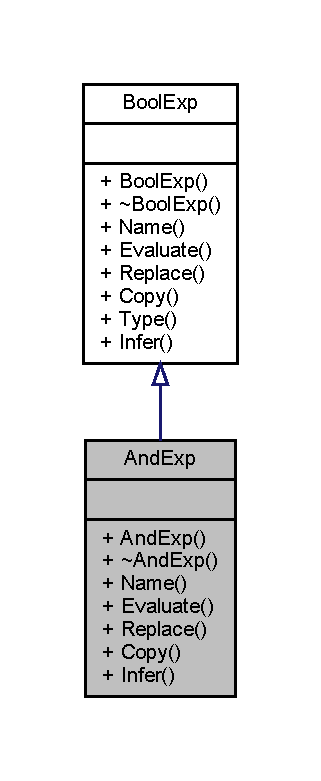
\includegraphics[width=154pt]{classAndExp__inherit__graph}
\end{center}
\end{figure}


Collaboration diagram for And\+Exp\+:
\nopagebreak
\begin{figure}[H]
\begin{center}
\leavevmode
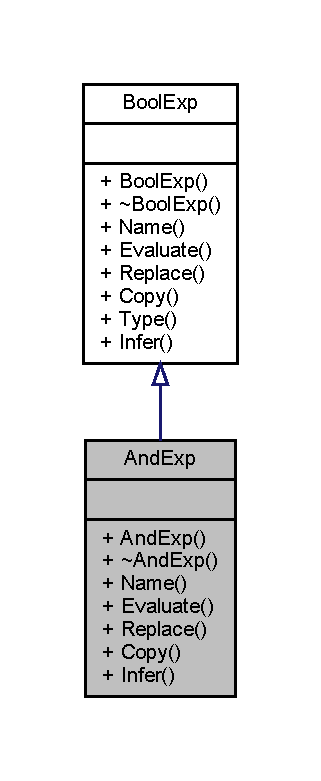
\includegraphics[width=154pt]{classAndExp__coll__graph}
\end{center}
\end{figure}
\subsection*{Public Member Functions}
\begin{DoxyCompactItemize}
\item 
\mbox{\hyperlink{classAndExp_a5a3124ff6fd4adca49a702f075100607}{And\+Exp}} (shared\+\_\+ptr$<$ \mbox{\hyperlink{classBoolExp}{Bool\+Exp}} $>$ op1, shared\+\_\+ptr$<$ \mbox{\hyperlink{classBoolExp}{Bool\+Exp}} $>$ op2)
\item 
virtual \mbox{\hyperlink{classAndExp_ab42437c5641d21c116bf0c90532b9075}{$\sim$\+And\+Exp}} ()
\item 
virtual string \mbox{\hyperlink{classAndExp_ac930ab2d9098904596aea6b2b6429d90}{Name}} () const
\item 
virtual bool \mbox{\hyperlink{classAndExp_a7708cad60cf9b0913d30a7164ed8aceb}{Evaluate}} (\mbox{\hyperlink{classContext}{Context}} \&con)
\item 
virtual shared\+\_\+ptr$<$ \mbox{\hyperlink{classBoolExp}{Bool\+Exp}} $>$ \mbox{\hyperlink{classAndExp_ac6176c316c96da57f587fe7731fc414b}{Replace}} (string name, \mbox{\hyperlink{classBoolExp}{Bool\+Exp}} \&exp)
\item 
virtual shared\+\_\+ptr$<$ \mbox{\hyperlink{classBoolExp}{Bool\+Exp}} $>$ \mbox{\hyperlink{classAndExp_a86a369f7f3bf7d4d157b9f0df9e6a315}{Copy}} () const
\item 
virtual \mbox{\hyperlink{structBoolReturn}{Bool\+Return}} \mbox{\hyperlink{classAndExp_a26390e42318a13aa0f03a4e5ccbb0270}{Infer}} ()
\end{DoxyCompactItemize}


\subsection{Detailed Description}
\mbox{\hyperlink{classAndExp}{And\+Exp}}\textquotesingle{}s are derived from \mbox{\hyperlink{classBoolExp}{Bool\+Exp}}\textquotesingle{}s they implement the logical proposition (A\&B) 

\subsection{Constructor \& Destructor Documentation}
\mbox{\Hypertarget{classAndExp_a5a3124ff6fd4adca49a702f075100607}\label{classAndExp_a5a3124ff6fd4adca49a702f075100607}} 
\index{And\+Exp@{And\+Exp}!And\+Exp@{And\+Exp}}
\index{And\+Exp@{And\+Exp}!And\+Exp@{And\+Exp}}
\subsubsection{\texorpdfstring{And\+Exp()}{AndExp()}}
{\footnotesize\ttfamily And\+Exp\+::\+And\+Exp (\begin{DoxyParamCaption}\item[{shared\+\_\+ptr$<$ \mbox{\hyperlink{classBoolExp}{Bool\+Exp}} $>$}]{op1,  }\item[{shared\+\_\+ptr$<$ \mbox{\hyperlink{classBoolExp}{Bool\+Exp}} $>$}]{op2 }\end{DoxyParamCaption})}

Constructs the specified \mbox{\hyperlink{classAndExp}{And\+Exp}} 
\begin{DoxyParams}{Parameters}
{\em op1} & becomes the left hand operand \\
\hline
{\em op2} & becomes the right hand operand \\
\hline
\end{DoxyParams}
\mbox{\Hypertarget{classAndExp_ab42437c5641d21c116bf0c90532b9075}\label{classAndExp_ab42437c5641d21c116bf0c90532b9075}} 
\index{And\+Exp@{And\+Exp}!````~And\+Exp@{$\sim$\+And\+Exp}}
\index{````~And\+Exp@{$\sim$\+And\+Exp}!And\+Exp@{And\+Exp}}
\subsubsection{\texorpdfstring{$\sim$\+And\+Exp()}{~AndExp()}}
{\footnotesize\ttfamily And\+Exp\+::$\sim$\+And\+Exp (\begin{DoxyParamCaption}{ }\end{DoxyParamCaption})\hspace{0.3cm}{\ttfamily [virtual]}}

The \mbox{\hyperlink{classAndExp}{And\+Exp}} destructor 

\subsection{Member Function Documentation}
\mbox{\Hypertarget{classAndExp_a86a369f7f3bf7d4d157b9f0df9e6a315}\label{classAndExp_a86a369f7f3bf7d4d157b9f0df9e6a315}} 
\index{And\+Exp@{And\+Exp}!Copy@{Copy}}
\index{Copy@{Copy}!And\+Exp@{And\+Exp}}
\subsubsection{\texorpdfstring{Copy()}{Copy()}}
{\footnotesize\ttfamily shared\+\_\+ptr$<$ \mbox{\hyperlink{classBoolExp}{Bool\+Exp}} $>$ And\+Exp\+::\+Copy (\begin{DoxyParamCaption}{ }\end{DoxyParamCaption}) const\hspace{0.3cm}{\ttfamily [virtual]}}

Create a copy of this \mbox{\hyperlink{classAndExp}{And\+Exp}} \begin{DoxyReturn}{Returns}
returns the copy of this \mbox{\hyperlink{classAndExp}{And\+Exp}} 
\end{DoxyReturn}


Implements \mbox{\hyperlink{classBoolExp_a846c30d1730cf645a040978a4cf7cdbb}{Bool\+Exp}}.

\mbox{\Hypertarget{classAndExp_a7708cad60cf9b0913d30a7164ed8aceb}\label{classAndExp_a7708cad60cf9b0913d30a7164ed8aceb}} 
\index{And\+Exp@{And\+Exp}!Evaluate@{Evaluate}}
\index{Evaluate@{Evaluate}!And\+Exp@{And\+Exp}}
\subsubsection{\texorpdfstring{Evaluate()}{Evaluate()}}
{\footnotesize\ttfamily bool And\+Exp\+::\+Evaluate (\begin{DoxyParamCaption}\item[{\mbox{\hyperlink{classContext}{Context}} \&}]{con }\end{DoxyParamCaption})\hspace{0.3cm}{\ttfamily [virtual]}}

Recursively evaluates the \mbox{\hyperlink{classAndExp}{And\+Exp}} via (op1.\+Evaluate() \&\& op2.\+Evaluate()) 
\begin{DoxyParams}{Parameters}
{\em con} & is the \mbox{\hyperlink{classContext}{Context}} class which maps variables to values \\
\hline
\end{DoxyParams}
\begin{DoxyReturn}{Returns}
returns the evaluation of the \mbox{\hyperlink{classBoolExp}{Bool\+Exp}} as a boolean 
\end{DoxyReturn}


Implements \mbox{\hyperlink{classBoolExp_a591fb5f9cb849e0f56e596406a9a10d0}{Bool\+Exp}}.

\mbox{\Hypertarget{classAndExp_a26390e42318a13aa0f03a4e5ccbb0270}\label{classAndExp_a26390e42318a13aa0f03a4e5ccbb0270}} 
\index{And\+Exp@{And\+Exp}!Infer@{Infer}}
\index{Infer@{Infer}!And\+Exp@{And\+Exp}}
\subsubsection{\texorpdfstring{Infer()}{Infer()}}
{\footnotesize\ttfamily \mbox{\hyperlink{structBoolReturn}{Bool\+Return}} And\+Exp\+::\+Infer (\begin{DoxyParamCaption}{ }\end{DoxyParamCaption})\hspace{0.3cm}{\ttfamily [virtual]}}

Make an inference from this \mbox{\hyperlink{classAndExp}{And\+Exp}} \begin{DoxyReturn}{Returns}
returns a \mbox{\hyperlink{structBoolReturn}{Bool\+Return}} with both operands set to the operands of this \mbox{\hyperlink{classAndExp}{And\+Exp}} 
\end{DoxyReturn}


Implements \mbox{\hyperlink{classBoolExp_a0e5d4a241332ae72d083645e4b71e0e6}{Bool\+Exp}}.

\mbox{\Hypertarget{classAndExp_ac930ab2d9098904596aea6b2b6429d90}\label{classAndExp_ac930ab2d9098904596aea6b2b6429d90}} 
\index{And\+Exp@{And\+Exp}!Name@{Name}}
\index{Name@{Name}!And\+Exp@{And\+Exp}}
\subsubsection{\texorpdfstring{Name()}{Name()}}
{\footnotesize\ttfamily string And\+Exp\+::\+Name (\begin{DoxyParamCaption}{ }\end{DoxyParamCaption}) const\hspace{0.3cm}{\ttfamily [virtual]}}

Recursively retrieves and returns a string representation of the \mbox{\hyperlink{classAndExp}{And\+Exp}} \begin{DoxyReturn}{Returns}
returns the name of this \mbox{\hyperlink{classAndExp}{And\+Exp}} as a string 
\end{DoxyReturn}


Implements \mbox{\hyperlink{classBoolExp_a3fdb64a9b8fd54e33d755ff4a577d11a}{Bool\+Exp}}.

\mbox{\Hypertarget{classAndExp_ac6176c316c96da57f587fe7731fc414b}\label{classAndExp_ac6176c316c96da57f587fe7731fc414b}} 
\index{And\+Exp@{And\+Exp}!Replace@{Replace}}
\index{Replace@{Replace}!And\+Exp@{And\+Exp}}
\subsubsection{\texorpdfstring{Replace()}{Replace()}}
{\footnotesize\ttfamily shared\+\_\+ptr$<$ \mbox{\hyperlink{classBoolExp}{Bool\+Exp}} $>$ And\+Exp\+::\+Replace (\begin{DoxyParamCaption}\item[{string}]{name,  }\item[{\mbox{\hyperlink{classBoolExp}{Bool\+Exp}} \&}]{exp }\end{DoxyParamCaption})\hspace{0.3cm}{\ttfamily [virtual]}}

Left in for possible future usage see \mbox{\hyperlink{classBoolExp}{Bool\+Exp}} explanation 
\begin{DoxyParams}{Parameters}
{\em name} & the name to use for replacement \\
\hline
{\em exp} & the expression to use for replacement \\
\hline
\end{DoxyParams}
\begin{DoxyReturn}{Returns}
returns the new \mbox{\hyperlink{classBoolExp}{Bool\+Exp}} 
\end{DoxyReturn}


Implements \mbox{\hyperlink{classBoolExp_a6448b7121c238759cc9cc8e48d6f8773}{Bool\+Exp}}.



The documentation for this class was generated from the following files\+:\begin{DoxyCompactItemize}
\item 
\mbox{\hyperlink{andexp_8h}{andexp.\+h}}\item 
\mbox{\hyperlink{andexp_8cpp}{andexp.\+cpp}}\end{DoxyCompactItemize}

\hypertarget{classBoolExp}{}\section{Bool\+Exp Class Reference}
\label{classBoolExp}\index{Bool\+Exp@{Bool\+Exp}}


{\ttfamily \#include $<$boolexp.\+h$>$}



Inheritance diagram for Bool\+Exp\+:
\nopagebreak
\begin{figure}[H]
\begin{center}
\leavevmode
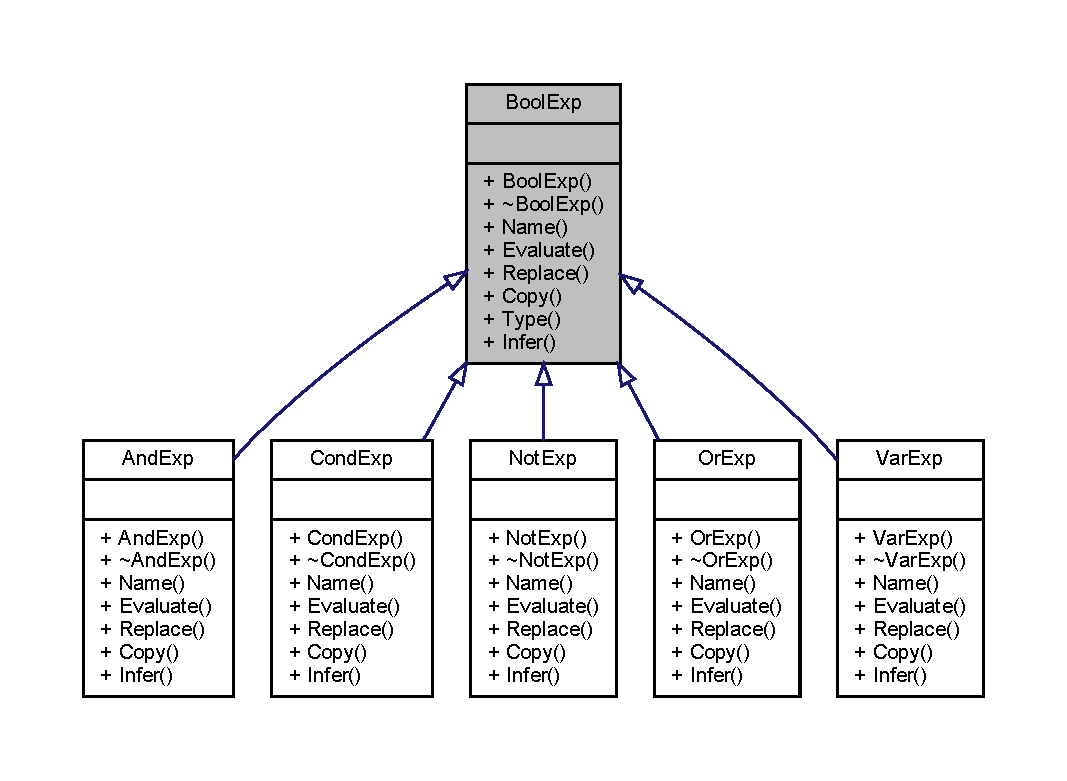
\includegraphics[width=350pt]{classBoolExp__inherit__graph}
\end{center}
\end{figure}


Collaboration diagram for Bool\+Exp\+:
\nopagebreak
\begin{figure}[H]
\begin{center}
\leavevmode
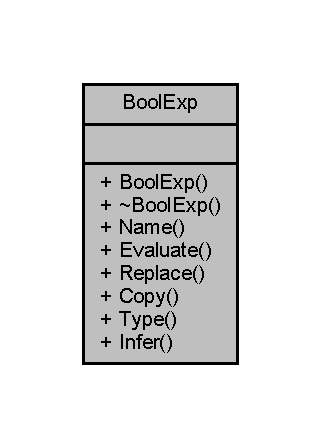
\includegraphics[width=154pt]{classBoolExp__coll__graph}
\end{center}
\end{figure}
\subsection*{Public Member Functions}
\begin{DoxyCompactItemize}
\item 
\mbox{\hyperlink{classBoolExp_afe8ce549303b55538b376f0975c2cd25}{Bool\+Exp}} (\mbox{\hyperlink{boolexp_8h_ac6a79184a0a7c1d2e3ea745512aa2d0c}{Prop\+Type}})
\item 
virtual \mbox{\hyperlink{classBoolExp_a3172fb0a33eba2f75c3737173df94066}{$\sim$\+Bool\+Exp}} ()
\item 
virtual string \mbox{\hyperlink{classBoolExp_a3fdb64a9b8fd54e33d755ff4a577d11a}{Name}} () const =0
\item 
virtual bool \mbox{\hyperlink{classBoolExp_a591fb5f9cb849e0f56e596406a9a10d0}{Evaluate}} (\mbox{\hyperlink{classContext}{Context}} \&con)=0
\item 
virtual shared\+\_\+ptr$<$ \mbox{\hyperlink{classBoolExp}{Bool\+Exp}} $>$ \mbox{\hyperlink{classBoolExp_a6448b7121c238759cc9cc8e48d6f8773}{Replace}} (string str, \mbox{\hyperlink{classBoolExp}{Bool\+Exp}} \&bol)=0
\item 
virtual shared\+\_\+ptr$<$ \mbox{\hyperlink{classBoolExp}{Bool\+Exp}} $>$ \mbox{\hyperlink{classBoolExp_a846c30d1730cf645a040978a4cf7cdbb}{Copy}} () const =0
\item 
virtual \mbox{\hyperlink{boolexp_8h_ac6a79184a0a7c1d2e3ea745512aa2d0c}{Prop\+Type}} \mbox{\hyperlink{classBoolExp_a1a6d410fe97a2b1b9452dd87a13b3082}{Type}} () const
\item 
virtual \mbox{\hyperlink{structBoolReturn}{Bool\+Return}} \mbox{\hyperlink{classBoolExp_a0e5d4a241332ae72d083645e4b71e0e6}{Infer}} ()=0
\end{DoxyCompactItemize}


\subsection{Detailed Description}
A \mbox{\hyperlink{classBoolExp}{Bool\+Exp}} is an abstract base class for derived boolean logic expression classes 

\subsection{Constructor \& Destructor Documentation}
\mbox{\Hypertarget{classBoolExp_afe8ce549303b55538b376f0975c2cd25}\label{classBoolExp_afe8ce549303b55538b376f0975c2cd25}} 
\index{Bool\+Exp@{Bool\+Exp}!Bool\+Exp@{Bool\+Exp}}
\index{Bool\+Exp@{Bool\+Exp}!Bool\+Exp@{Bool\+Exp}}
\subsubsection{\texorpdfstring{Bool\+Exp()}{BoolExp()}}
{\footnotesize\ttfamily Bool\+Exp\+::\+Bool\+Exp (\begin{DoxyParamCaption}\item[{\mbox{\hyperlink{boolexp_8h_ac6a79184a0a7c1d2e3ea745512aa2d0c}{Prop\+Type}}}]{p }\end{DoxyParamCaption})}

Derived classes supply the corresponding proposition types to \mbox{\hyperlink{classBoolExp}{Bool\+Exp}}\textquotesingle{}s via this constructor \mbox{\Hypertarget{classBoolExp_a3172fb0a33eba2f75c3737173df94066}\label{classBoolExp_a3172fb0a33eba2f75c3737173df94066}} 
\index{Bool\+Exp@{Bool\+Exp}!````~Bool\+Exp@{$\sim$\+Bool\+Exp}}
\index{````~Bool\+Exp@{$\sim$\+Bool\+Exp}!Bool\+Exp@{Bool\+Exp}}
\subsubsection{\texorpdfstring{$\sim$\+Bool\+Exp()}{~BoolExp()}}
{\footnotesize\ttfamily Bool\+Exp\+::$\sim$\+Bool\+Exp (\begin{DoxyParamCaption}{ }\end{DoxyParamCaption})\hspace{0.3cm}{\ttfamily [virtual]}}

The destructor for a \mbox{\hyperlink{classBoolExp}{Bool\+Exp}} 

\subsection{Member Function Documentation}
\mbox{\Hypertarget{classBoolExp_a846c30d1730cf645a040978a4cf7cdbb}\label{classBoolExp_a846c30d1730cf645a040978a4cf7cdbb}} 
\index{Bool\+Exp@{Bool\+Exp}!Copy@{Copy}}
\index{Copy@{Copy}!Bool\+Exp@{Bool\+Exp}}
\subsubsection{\texorpdfstring{Copy()}{Copy()}}
{\footnotesize\ttfamily virtual shared\+\_\+ptr$<$\mbox{\hyperlink{classBoolExp}{Bool\+Exp}}$>$ Bool\+Exp\+::\+Copy (\begin{DoxyParamCaption}{ }\end{DoxyParamCaption}) const\hspace{0.3cm}{\ttfamily [pure virtual]}}

Create a copy of this \mbox{\hyperlink{classAndExp}{And\+Exp}} \begin{DoxyReturn}{Returns}
returns the copy of this \mbox{\hyperlink{classBoolExp}{Bool\+Exp}} 
\end{DoxyReturn}


Implemented in \mbox{\hyperlink{classAndExp_a86a369f7f3bf7d4d157b9f0df9e6a315}{And\+Exp}}, \mbox{\hyperlink{classNotExp_adb36074264fb55186f781680cb6c35f9}{Not\+Exp}}, \mbox{\hyperlink{classCondExp_a07dc28d880912ea9553c75ebf26431e8}{Cond\+Exp}}, \mbox{\hyperlink{classOrExp_a142f557d9b95c4464dbd9167dbb9fe51}{Or\+Exp}}, and \mbox{\hyperlink{classVarExp_ad93ffa6aa927bc41c9765bc37b4d0a63}{Var\+Exp}}.

\mbox{\Hypertarget{classBoolExp_a591fb5f9cb849e0f56e596406a9a10d0}\label{classBoolExp_a591fb5f9cb849e0f56e596406a9a10d0}} 
\index{Bool\+Exp@{Bool\+Exp}!Evaluate@{Evaluate}}
\index{Evaluate@{Evaluate}!Bool\+Exp@{Bool\+Exp}}
\subsubsection{\texorpdfstring{Evaluate()}{Evaluate()}}
{\footnotesize\ttfamily virtual bool Bool\+Exp\+::\+Evaluate (\begin{DoxyParamCaption}\item[{\mbox{\hyperlink{classContext}{Context}} \&}]{con }\end{DoxyParamCaption})\hspace{0.3cm}{\ttfamily [pure virtual]}}

\mbox{\hyperlink{classBoolExp}{Bool\+Exp}}\textquotesingle{}s are meant to be evaluated in a recursive manner like how they are printed but implementation of this feature is determined by the derived classes themselves 
\begin{DoxyParams}{Parameters}
{\em con} & is a class which maps variable names to values \\
\hline
\end{DoxyParams}
\begin{DoxyReturn}{Returns}
returns the evaluation of the \mbox{\hyperlink{classBoolExp}{Bool\+Exp}} as a boolean 
\end{DoxyReturn}


Implemented in \mbox{\hyperlink{classAndExp_a7708cad60cf9b0913d30a7164ed8aceb}{And\+Exp}}, \mbox{\hyperlink{classNotExp_a4bf3ac9a898127b4d0c63db2a5f7a82f}{Not\+Exp}}, \mbox{\hyperlink{classCondExp_a36c86af1adba98b0ab7d15fa53e4027f}{Cond\+Exp}}, \mbox{\hyperlink{classOrExp_a2056a325b87621e2a3d0afff79c4163e}{Or\+Exp}}, and \mbox{\hyperlink{classVarExp_af9d73e76a255123e00d5ebb1ae703188}{Var\+Exp}}.

\mbox{\Hypertarget{classBoolExp_a0e5d4a241332ae72d083645e4b71e0e6}\label{classBoolExp_a0e5d4a241332ae72d083645e4b71e0e6}} 
\index{Bool\+Exp@{Bool\+Exp}!Infer@{Infer}}
\index{Infer@{Infer}!Bool\+Exp@{Bool\+Exp}}
\subsubsection{\texorpdfstring{Infer()}{Infer()}}
{\footnotesize\ttfamily virtual \mbox{\hyperlink{structBoolReturn}{Bool\+Return}} Bool\+Exp\+::\+Infer (\begin{DoxyParamCaption}{ }\end{DoxyParamCaption})\hspace{0.3cm}{\ttfamily [pure virtual]}}

Infer allows \mbox{\hyperlink{classBoolExp}{Bool\+Exp}}\textquotesingle{}s to be modified via inference rules. Generally a \mbox{\hyperlink{classBoolExp}{Bool\+Exp}} Just returns its children but having this as a virtual method allows a \mbox{\hyperlink{classBoolExp}{Bool\+Exp}} to self modify upon inference if needed \begin{DoxyReturn}{Returns}
returns a properly configured \mbox{\hyperlink{structBoolReturn}{Bool\+Return}} 
\end{DoxyReturn}


Implemented in \mbox{\hyperlink{classAndExp_a26390e42318a13aa0f03a4e5ccbb0270}{And\+Exp}}, \mbox{\hyperlink{classNotExp_ad7ec5fee6dd934a3db7f72cc9e0b809a}{Not\+Exp}}, \mbox{\hyperlink{classCondExp_a3824041035f12f58e583181b57491668}{Cond\+Exp}}, \mbox{\hyperlink{classOrExp_aa3b98be68c00bc0c43a9eec5a47cdec9}{Or\+Exp}}, and \mbox{\hyperlink{classVarExp_a6c3e1736ade0456d23085923bc3fef61}{Var\+Exp}}.

\mbox{\Hypertarget{classBoolExp_a3fdb64a9b8fd54e33d755ff4a577d11a}\label{classBoolExp_a3fdb64a9b8fd54e33d755ff4a577d11a}} 
\index{Bool\+Exp@{Bool\+Exp}!Name@{Name}}
\index{Name@{Name}!Bool\+Exp@{Bool\+Exp}}
\subsubsection{\texorpdfstring{Name()}{Name()}}
{\footnotesize\ttfamily virtual string Bool\+Exp\+::\+Name (\begin{DoxyParamCaption}{ }\end{DoxyParamCaption}) const\hspace{0.3cm}{\ttfamily [pure virtual]}}

Returns the name of the formula by calling this method recursively on nested boolexp\textquotesingle{}s every \mbox{\hyperlink{classBoolExp}{Bool\+Exp}} supports this so any arbitrary tree of \mbox{\hyperlink{classBoolExp}{Bool\+Exp}}\textquotesingle{}s can be printed. \begin{DoxyReturn}{Returns}
returns the name of this \mbox{\hyperlink{classBoolExp}{Bool\+Exp}} as a string 
\end{DoxyReturn}


Implemented in \mbox{\hyperlink{classAndExp_ac930ab2d9098904596aea6b2b6429d90}{And\+Exp}}, \mbox{\hyperlink{classNotExp_a7363cb79787e02ca362a4ea6cdd6d7e2}{Not\+Exp}}, \mbox{\hyperlink{classOrExp_a8e535ae2da801bf5a4e8c9fbf3426a8b}{Or\+Exp}}, \mbox{\hyperlink{classCondExp_a556da724a343a45e1bab5da0a3f8a091}{Cond\+Exp}}, and \mbox{\hyperlink{classVarExp_af50f77454d193ebfd7633f5f20becaf4}{Var\+Exp}}.

\mbox{\Hypertarget{classBoolExp_a6448b7121c238759cc9cc8e48d6f8773}\label{classBoolExp_a6448b7121c238759cc9cc8e48d6f8773}} 
\index{Bool\+Exp@{Bool\+Exp}!Replace@{Replace}}
\index{Replace@{Replace}!Bool\+Exp@{Bool\+Exp}}
\subsubsection{\texorpdfstring{Replace()}{Replace()}}
{\footnotesize\ttfamily virtual shared\+\_\+ptr$<$\mbox{\hyperlink{classBoolExp}{Bool\+Exp}}$>$ Bool\+Exp\+::\+Replace (\begin{DoxyParamCaption}\item[{string}]{str,  }\item[{\mbox{\hyperlink{classBoolExp}{Bool\+Exp}} \&}]{bol }\end{DoxyParamCaption})\hspace{0.3cm}{\ttfamily [pure virtual]}}

All \mbox{\hyperlink{classBoolExp}{Bool\+Exp}}\textquotesingle{}s support a replace operation which is implemented by derived classes note that I did not find this method very useful but it is left in due to possibly being useful in the future 
\begin{DoxyParams}{Parameters}
{\em str} & receives the name of bol \\
\hline
{\em bol} & receives a \mbox{\hyperlink{classBoolExp}{Bool\+Exp}} \\
\hline
\end{DoxyParams}
\begin{DoxyReturn}{Returns}
returns the new \mbox{\hyperlink{classBoolExp}{Bool\+Exp}} 
\end{DoxyReturn}


Implemented in \mbox{\hyperlink{classAndExp_ac6176c316c96da57f587fe7731fc414b}{And\+Exp}}, \mbox{\hyperlink{classNotExp_aeba42c37b59e0eaaf981260e4b163d98}{Not\+Exp}}, \mbox{\hyperlink{classCondExp_a0bbcb0b6822b47bee1baa09d7c88f4d0}{Cond\+Exp}}, \mbox{\hyperlink{classOrExp_a256171f2cf3d3165745d6df9390d9ab7}{Or\+Exp}}, and \mbox{\hyperlink{classVarExp_a0b716a76069a7fad3b99b86a9bd9d331}{Var\+Exp}}.

\mbox{\Hypertarget{classBoolExp_a1a6d410fe97a2b1b9452dd87a13b3082}\label{classBoolExp_a1a6d410fe97a2b1b9452dd87a13b3082}} 
\index{Bool\+Exp@{Bool\+Exp}!Type@{Type}}
\index{Type@{Type}!Bool\+Exp@{Bool\+Exp}}
\subsubsection{\texorpdfstring{Type()}{Type()}}
{\footnotesize\ttfamily \mbox{\hyperlink{boolexp_8h_ac6a79184a0a7c1d2e3ea745512aa2d0c}{Prop\+Type}} Bool\+Exp\+::\+Type (\begin{DoxyParamCaption}{ }\end{DoxyParamCaption}) const\hspace{0.3cm}{\ttfamily [virtual]}}

Every \mbox{\hyperlink{classBoolExp}{Bool\+Exp}} includes information pertaining to its type, every \mbox{\hyperlink{classBoolExp}{Bool\+Exp}}\textquotesingle{}s type is determined by its outermost type \begin{DoxyReturn}{Returns}
returns the type of the outermost formula 
\end{DoxyReturn}


The documentation for this class was generated from the following files\+:\begin{DoxyCompactItemize}
\item 
\mbox{\hyperlink{boolexp_8h}{boolexp.\+h}}\item 
\mbox{\hyperlink{boolexp_8cpp}{boolexp.\+cpp}}\end{DoxyCompactItemize}

\hypertarget{structBoolReturn}{}\section{Bool\+Return Struct Reference}
\label{structBoolReturn}\index{Bool\+Return@{Bool\+Return}}


{\ttfamily \#include $<$boolexp.\+h$>$}



Collaboration diagram for Bool\+Return\+:
\nopagebreak
\begin{figure}[H]
\begin{center}
\leavevmode
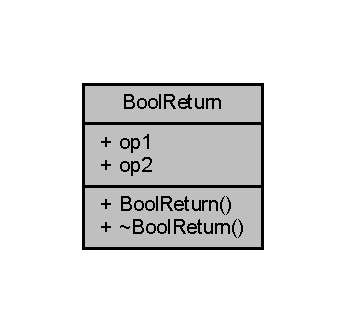
\includegraphics[width=166pt]{structBoolReturn__coll__graph}
\end{center}
\end{figure}
\subsection*{Public Member Functions}
\begin{DoxyCompactItemize}
\item 
\mbox{\hyperlink{structBoolReturn_a1369d14d90011e707b0823656f7e2f55}{Bool\+Return}} (shared\+\_\+ptr$<$ \mbox{\hyperlink{classBoolExp}{Bool\+Exp}} $>$, shared\+\_\+ptr$<$ \mbox{\hyperlink{classBoolExp}{Bool\+Exp}} $>$)
\item 
\mbox{\hyperlink{structBoolReturn_ade34b5e173d4c599b9f273848d8582b4}{$\sim$\+Bool\+Return}} ()
\end{DoxyCompactItemize}
\subsection*{Public Attributes}
\begin{DoxyCompactItemize}
\item 
shared\+\_\+ptr$<$ \mbox{\hyperlink{classBoolExp}{Bool\+Exp}} $>$ \mbox{\hyperlink{structBoolReturn_a16f84cab94347ac45de9dac81a932a66}{op1}}
\item 
shared\+\_\+ptr$<$ \mbox{\hyperlink{classBoolExp}{Bool\+Exp}} $>$ \mbox{\hyperlink{structBoolReturn_aac386029dd2fe9c58e818c359143c124}{op2}}
\end{DoxyCompactItemize}


\subsection{Detailed Description}
\mbox{\hyperlink{structBoolReturn}{Bool\+Return}} is a convenience struct for returning pointers to the members of a \mbox{\hyperlink{classBoolExp}{Bool\+Exp}} this feature is heavily used in the prover class 

\subsection{Constructor \& Destructor Documentation}
\mbox{\Hypertarget{structBoolReturn_a1369d14d90011e707b0823656f7e2f55}\label{structBoolReturn_a1369d14d90011e707b0823656f7e2f55}} 
\index{Bool\+Return@{Bool\+Return}!Bool\+Return@{Bool\+Return}}
\index{Bool\+Return@{Bool\+Return}!Bool\+Return@{Bool\+Return}}
\subsubsection{\texorpdfstring{Bool\+Return()}{BoolReturn()}}
{\footnotesize\ttfamily Bool\+Return\+::\+Bool\+Return (\begin{DoxyParamCaption}\item[{shared\+\_\+ptr$<$ \mbox{\hyperlink{classBoolExp}{Bool\+Exp}} $>$}]{o1,  }\item[{shared\+\_\+ptr$<$ \mbox{\hyperlink{classBoolExp}{Bool\+Exp}} $>$}]{o2 }\end{DoxyParamCaption})}

The \mbox{\hyperlink{structBoolReturn}{Bool\+Return}} constructor initializes the two shared\+\_\+ptr\textquotesingle{}s to point to the requested members of a chosen \mbox{\hyperlink{classBoolExp}{Bool\+Exp}} \mbox{\Hypertarget{structBoolReturn_ade34b5e173d4c599b9f273848d8582b4}\label{structBoolReturn_ade34b5e173d4c599b9f273848d8582b4}} 
\index{Bool\+Return@{Bool\+Return}!````~Bool\+Return@{$\sim$\+Bool\+Return}}
\index{````~Bool\+Return@{$\sim$\+Bool\+Return}!Bool\+Return@{Bool\+Return}}
\subsubsection{\texorpdfstring{$\sim$\+Bool\+Return()}{~BoolReturn()}}
{\footnotesize\ttfamily Bool\+Return\+::$\sim$\+Bool\+Return (\begin{DoxyParamCaption}{ }\end{DoxyParamCaption})\hspace{0.3cm}{\ttfamily [inline]}}

The \mbox{\hyperlink{structBoolReturn}{Bool\+Return}} destructor 

\subsection{Member Data Documentation}
\mbox{\Hypertarget{structBoolReturn_a16f84cab94347ac45de9dac81a932a66}\label{structBoolReturn_a16f84cab94347ac45de9dac81a932a66}} 
\index{Bool\+Return@{Bool\+Return}!op1@{op1}}
\index{op1@{op1}!Bool\+Return@{Bool\+Return}}
\subsubsection{\texorpdfstring{op1}{op1}}
{\footnotesize\ttfamily shared\+\_\+ptr$<$\mbox{\hyperlink{classBoolExp}{Bool\+Exp}}$>$ Bool\+Return\+::op1}

op1 is used for the left hand member of a \mbox{\hyperlink{classBoolExp}{Bool\+Exp}} or the only member of a unary \mbox{\hyperlink{classBoolExp}{Bool\+Exp}} \mbox{\Hypertarget{structBoolReturn_aac386029dd2fe9c58e818c359143c124}\label{structBoolReturn_aac386029dd2fe9c58e818c359143c124}} 
\index{Bool\+Return@{Bool\+Return}!op2@{op2}}
\index{op2@{op2}!Bool\+Return@{Bool\+Return}}
\subsubsection{\texorpdfstring{op2}{op2}}
{\footnotesize\ttfamily shared\+\_\+ptr$<$\mbox{\hyperlink{classBoolExp}{Bool\+Exp}}$>$ Bool\+Return\+::op2}

op2 is used for the right hand member of a \mbox{\hyperlink{classBoolExp}{Bool\+Exp}} or the only member of a unary \mbox{\hyperlink{classBoolExp}{Bool\+Exp}} 

The documentation for this struct was generated from the following files\+:\begin{DoxyCompactItemize}
\item 
\mbox{\hyperlink{boolexp_8h}{boolexp.\+h}}\item 
\mbox{\hyperlink{boolexp_8cpp}{boolexp.\+cpp}}\end{DoxyCompactItemize}

\hypertarget{classCondExp}{}\section{Cond\+Exp Class Reference}
\label{classCondExp}\index{Cond\+Exp@{Cond\+Exp}}


{\ttfamily \#include $<$condexp.\+h$>$}



Inheritance diagram for Cond\+Exp\+:
\nopagebreak
\begin{figure}[H]
\begin{center}
\leavevmode
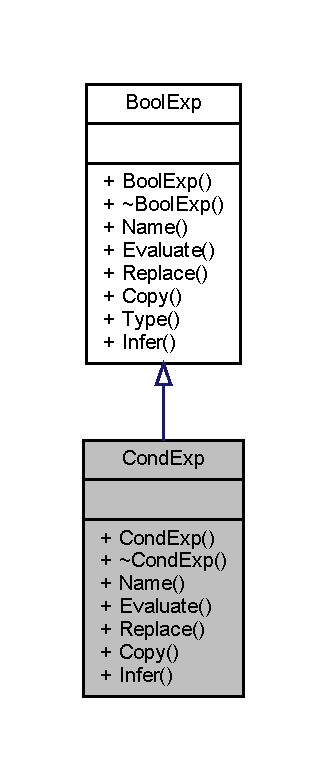
\includegraphics[width=157pt]{classCondExp__inherit__graph}
\end{center}
\end{figure}


Collaboration diagram for Cond\+Exp\+:
\nopagebreak
\begin{figure}[H]
\begin{center}
\leavevmode
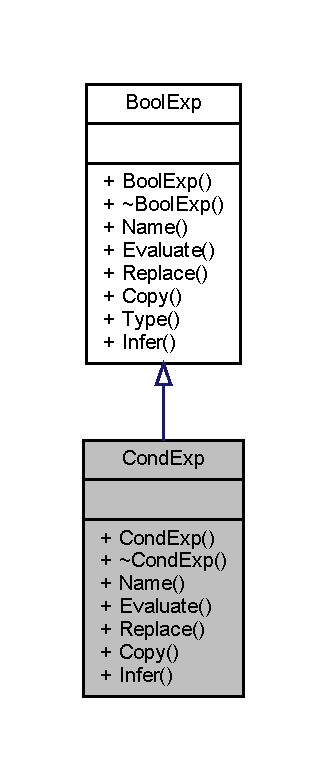
\includegraphics[width=157pt]{classCondExp__coll__graph}
\end{center}
\end{figure}
\subsection*{Public Member Functions}
\begin{DoxyCompactItemize}
\item 
\mbox{\hyperlink{classCondExp_a7c531f5e34f68fc5d5436a0a521de0b5}{Cond\+Exp}} (shared\+\_\+ptr$<$ \mbox{\hyperlink{classBoolExp}{Bool\+Exp}} $>$, shared\+\_\+ptr$<$ \mbox{\hyperlink{classBoolExp}{Bool\+Exp}} $>$)
\item 
virtual \mbox{\hyperlink{classCondExp_aad96be2ad7ce013bc05dfc77f541bf24}{$\sim$\+Cond\+Exp}} ()
\item 
virtual string \mbox{\hyperlink{classCondExp_a556da724a343a45e1bab5da0a3f8a091}{Name}} () const
\item 
virtual bool \mbox{\hyperlink{classCondExp_a36c86af1adba98b0ab7d15fa53e4027f}{Evaluate}} (\mbox{\hyperlink{classContext}{Context}} \&)
\item 
virtual shared\+\_\+ptr$<$ \mbox{\hyperlink{classBoolExp}{Bool\+Exp}} $>$ \mbox{\hyperlink{classCondExp_a0bbcb0b6822b47bee1baa09d7c88f4d0}{Replace}} (string, \mbox{\hyperlink{classBoolExp}{Bool\+Exp}} \&)
\item 
virtual shared\+\_\+ptr$<$ \mbox{\hyperlink{classBoolExp}{Bool\+Exp}} $>$ \mbox{\hyperlink{classCondExp_a07dc28d880912ea9553c75ebf26431e8}{Copy}} () const
\item 
virtual \mbox{\hyperlink{structBoolReturn}{Bool\+Return}} \mbox{\hyperlink{classCondExp_a3824041035f12f58e583181b57491668}{Infer}} ()
\end{DoxyCompactItemize}


\subsection{Detailed Description}
\mbox{\hyperlink{classCondExp}{Cond\+Exp}}\textquotesingle{}s are derived from \mbox{\hyperlink{classBoolExp}{Bool\+Exp}}\textquotesingle{}s they implement the logical proposition (A-\/$>$B) 

\subsection{Constructor \& Destructor Documentation}
\mbox{\Hypertarget{classCondExp_a7c531f5e34f68fc5d5436a0a521de0b5}\label{classCondExp_a7c531f5e34f68fc5d5436a0a521de0b5}} 
\index{Cond\+Exp@{Cond\+Exp}!Cond\+Exp@{Cond\+Exp}}
\index{Cond\+Exp@{Cond\+Exp}!Cond\+Exp@{Cond\+Exp}}
\subsubsection{\texorpdfstring{Cond\+Exp()}{CondExp()}}
{\footnotesize\ttfamily Cond\+Exp\+::\+Cond\+Exp (\begin{DoxyParamCaption}\item[{shared\+\_\+ptr$<$ \mbox{\hyperlink{classBoolExp}{Bool\+Exp}} $>$}]{op1,  }\item[{shared\+\_\+ptr$<$ \mbox{\hyperlink{classBoolExp}{Bool\+Exp}} $>$}]{op2 }\end{DoxyParamCaption})}

Constructs the specified \mbox{\hyperlink{classCondExp}{Cond\+Exp}} 
\begin{DoxyParams}{Parameters}
{\em op1} & becomes the left hand operand \\
\hline
{\em op2} & becomes the right hand operand \\
\hline
\end{DoxyParams}
\mbox{\Hypertarget{classCondExp_aad96be2ad7ce013bc05dfc77f541bf24}\label{classCondExp_aad96be2ad7ce013bc05dfc77f541bf24}} 
\index{Cond\+Exp@{Cond\+Exp}!````~Cond\+Exp@{$\sim$\+Cond\+Exp}}
\index{````~Cond\+Exp@{$\sim$\+Cond\+Exp}!Cond\+Exp@{Cond\+Exp}}
\subsubsection{\texorpdfstring{$\sim$\+Cond\+Exp()}{~CondExp()}}
{\footnotesize\ttfamily Cond\+Exp\+::$\sim$\+Cond\+Exp (\begin{DoxyParamCaption}{ }\end{DoxyParamCaption})\hspace{0.3cm}{\ttfamily [virtual]}}

The \mbox{\hyperlink{classCondExp}{Cond\+Exp}} destructor 

\subsection{Member Function Documentation}
\mbox{\Hypertarget{classCondExp_a07dc28d880912ea9553c75ebf26431e8}\label{classCondExp_a07dc28d880912ea9553c75ebf26431e8}} 
\index{Cond\+Exp@{Cond\+Exp}!Copy@{Copy}}
\index{Copy@{Copy}!Cond\+Exp@{Cond\+Exp}}
\subsubsection{\texorpdfstring{Copy()}{Copy()}}
{\footnotesize\ttfamily shared\+\_\+ptr$<$ \mbox{\hyperlink{classBoolExp}{Bool\+Exp}} $>$ Cond\+Exp\+::\+Copy (\begin{DoxyParamCaption}{ }\end{DoxyParamCaption}) const\hspace{0.3cm}{\ttfamily [virtual]}}

Create a copy of this \mbox{\hyperlink{classCondExp}{Cond\+Exp}} \begin{DoxyReturn}{Returns}
returns the copy of this \mbox{\hyperlink{classCondExp}{Cond\+Exp}} 
\end{DoxyReturn}


Implements \mbox{\hyperlink{classBoolExp_a846c30d1730cf645a040978a4cf7cdbb}{Bool\+Exp}}.

\mbox{\Hypertarget{classCondExp_a36c86af1adba98b0ab7d15fa53e4027f}\label{classCondExp_a36c86af1adba98b0ab7d15fa53e4027f}} 
\index{Cond\+Exp@{Cond\+Exp}!Evaluate@{Evaluate}}
\index{Evaluate@{Evaluate}!Cond\+Exp@{Cond\+Exp}}
\subsubsection{\texorpdfstring{Evaluate()}{Evaluate()}}
{\footnotesize\ttfamily bool Cond\+Exp\+::\+Evaluate (\begin{DoxyParamCaption}\item[{\mbox{\hyperlink{classContext}{Context}} \&}]{con }\end{DoxyParamCaption})\hspace{0.3cm}{\ttfamily [virtual]}}

Recursively evaluates the \mbox{\hyperlink{classOrExp}{Or\+Exp}} via (!op1.\mbox{\hyperlink{classCondExp_a36c86af1adba98b0ab7d15fa53e4027f}{Evaluate()}} $\vert$$\vert$ op2.\+Evaluate()) 
\begin{DoxyParams}{Parameters}
{\em con} & is the \mbox{\hyperlink{classContext}{Context}} class which maps variables to values \\
\hline
\end{DoxyParams}
\begin{DoxyReturn}{Returns}
returns the evaluation of the \mbox{\hyperlink{classBoolExp}{Bool\+Exp}} as a boolean 
\end{DoxyReturn}


Implements \mbox{\hyperlink{classBoolExp_a591fb5f9cb849e0f56e596406a9a10d0}{Bool\+Exp}}.

\mbox{\Hypertarget{classCondExp_a3824041035f12f58e583181b57491668}\label{classCondExp_a3824041035f12f58e583181b57491668}} 
\index{Cond\+Exp@{Cond\+Exp}!Infer@{Infer}}
\index{Infer@{Infer}!Cond\+Exp@{Cond\+Exp}}
\subsubsection{\texorpdfstring{Infer()}{Infer()}}
{\footnotesize\ttfamily \mbox{\hyperlink{structBoolReturn}{Bool\+Return}} Cond\+Exp\+::\+Infer (\begin{DoxyParamCaption}{ }\end{DoxyParamCaption})\hspace{0.3cm}{\ttfamily [virtual]}}

Make an inference from this \mbox{\hyperlink{classCondExp}{Cond\+Exp}} \begin{DoxyReturn}{Returns}
returns a \mbox{\hyperlink{structBoolReturn}{Bool\+Return}} with both operands set to the operands of this \mbox{\hyperlink{classCondExp}{Cond\+Exp}} 
\end{DoxyReturn}


Implements \mbox{\hyperlink{classBoolExp_a0e5d4a241332ae72d083645e4b71e0e6}{Bool\+Exp}}.

\mbox{\Hypertarget{classCondExp_a556da724a343a45e1bab5da0a3f8a091}\label{classCondExp_a556da724a343a45e1bab5da0a3f8a091}} 
\index{Cond\+Exp@{Cond\+Exp}!Name@{Name}}
\index{Name@{Name}!Cond\+Exp@{Cond\+Exp}}
\subsubsection{\texorpdfstring{Name()}{Name()}}
{\footnotesize\ttfamily string Cond\+Exp\+::\+Name (\begin{DoxyParamCaption}{ }\end{DoxyParamCaption}) const\hspace{0.3cm}{\ttfamily [virtual]}}

Recursively retrieves and returns a string representation of the \mbox{\hyperlink{classCondExp}{Cond\+Exp}} \begin{DoxyReturn}{Returns}
returns the name of this \mbox{\hyperlink{classCondExp}{Cond\+Exp}} as a string 
\end{DoxyReturn}


Implements \mbox{\hyperlink{classBoolExp_a3fdb64a9b8fd54e33d755ff4a577d11a}{Bool\+Exp}}.

\mbox{\Hypertarget{classCondExp_a0bbcb0b6822b47bee1baa09d7c88f4d0}\label{classCondExp_a0bbcb0b6822b47bee1baa09d7c88f4d0}} 
\index{Cond\+Exp@{Cond\+Exp}!Replace@{Replace}}
\index{Replace@{Replace}!Cond\+Exp@{Cond\+Exp}}
\subsubsection{\texorpdfstring{Replace()}{Replace()}}
{\footnotesize\ttfamily shared\+\_\+ptr$<$ \mbox{\hyperlink{classBoolExp}{Bool\+Exp}} $>$ Cond\+Exp\+::\+Replace (\begin{DoxyParamCaption}\item[{string}]{name,  }\item[{\mbox{\hyperlink{classBoolExp}{Bool\+Exp}} \&}]{exp }\end{DoxyParamCaption})\hspace{0.3cm}{\ttfamily [virtual]}}

Left in for possible future usage see \mbox{\hyperlink{classBoolExp}{Bool\+Exp}} explanation 
\begin{DoxyParams}{Parameters}
{\em name} & the name to use for replacement \\
\hline
{\em exp} & the expression to use for replacement \\
\hline
\end{DoxyParams}
\begin{DoxyReturn}{Returns}
returns the new \mbox{\hyperlink{classBoolExp}{Bool\+Exp}} 
\end{DoxyReturn}


Implements \mbox{\hyperlink{classBoolExp_a6448b7121c238759cc9cc8e48d6f8773}{Bool\+Exp}}.



The documentation for this class was generated from the following files\+:\begin{DoxyCompactItemize}
\item 
\mbox{\hyperlink{condexp_8h}{condexp.\+h}}\item 
\mbox{\hyperlink{condexp_8cpp}{condexp.\+cpp}}\end{DoxyCompactItemize}

\hypertarget{classContext}{}\section{Context Class Reference}
\label{classContext}\index{Context@{Context}}


{\ttfamily \#include $<$context.\+h$>$}



Collaboration diagram for Context\+:
\nopagebreak
\begin{figure}[H]
\begin{center}
\leavevmode
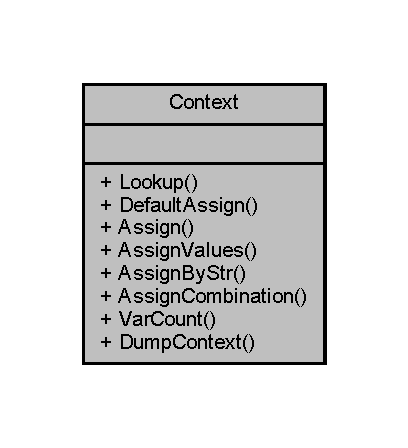
\includegraphics[width=196pt]{classContext__coll__graph}
\end{center}
\end{figure}
\subsection*{Public Member Functions}
\begin{DoxyCompactItemize}
\item 
bool \mbox{\hyperlink{classContext_adb549e858c14fd20ea21d12df224034b}{Lookup}} (string str) const
\item 
void \mbox{\hyperlink{classContext_abbc623520a3b4ec31c55ade44fddc953}{Default\+Assign}} (string str)
\item 
void \mbox{\hyperlink{classContext_a223eb7768e091ed328ac50cd7955a198}{Assign}} (shared\+\_\+ptr$<$ \mbox{\hyperlink{classVarExp}{Var\+Exp}} $>$ var, bool trf)
\item 
void \mbox{\hyperlink{classContext_a45f69da87ee7bc8843f6f99808e6686e}{Assign\+Values}} ()
\item 
void \mbox{\hyperlink{classContext_aa7bdd4c9b4aa512ac7d08dd58f5e13c0}{Assign\+By\+Str}} (string str, bool trf)
\item 
void \mbox{\hyperlink{classContext_abec0d3806d24c62690deb56803a70712}{Assign\+Combination}} (vector$<$ bool $>$ \&combination)
\item 
int \mbox{\hyperlink{classContext_a548788d37239de4a5e8a85a128c9a570}{Var\+Count}} ()
\item 
void \mbox{\hyperlink{classContext_ab61f6ccce5943b4aab6dac8cfdc9513c}{Dump\+Context}} ()
\end{DoxyCompactItemize}


\subsection{Detailed Description}
The \mbox{\hyperlink{classContext}{Context}} class is mainly used for mapping variables to values 

\subsection{Member Function Documentation}
\mbox{\Hypertarget{classContext_a223eb7768e091ed328ac50cd7955a198}\label{classContext_a223eb7768e091ed328ac50cd7955a198}} 
\index{Context@{Context}!Assign@{Assign}}
\index{Assign@{Assign}!Context@{Context}}
\subsubsection{\texorpdfstring{Assign()}{Assign()}}
{\footnotesize\ttfamily void Context\+::\+Assign (\begin{DoxyParamCaption}\item[{shared\+\_\+ptr$<$ \mbox{\hyperlink{classVarExp}{Var\+Exp}} $>$}]{var,  }\item[{bool}]{trf }\end{DoxyParamCaption})}

insert the \mbox{\hyperlink{classVarExp}{Var\+Exp}} var with the bool value of trf into the map 
\begin{DoxyParams}{Parameters}
{\em var} & the variable being inserted \\
\hline
{\em trf} & the value that var will receive \\
\hline
\end{DoxyParams}
\mbox{\Hypertarget{classContext_aa7bdd4c9b4aa512ac7d08dd58f5e13c0}\label{classContext_aa7bdd4c9b4aa512ac7d08dd58f5e13c0}} 
\index{Context@{Context}!Assign\+By\+Str@{Assign\+By\+Str}}
\index{Assign\+By\+Str@{Assign\+By\+Str}!Context@{Context}}
\subsubsection{\texorpdfstring{Assign\+By\+Str()}{AssignByStr()}}
{\footnotesize\ttfamily void Context\+::\+Assign\+By\+Str (\begin{DoxyParamCaption}\item[{string}]{str,  }\item[{bool}]{trf }\end{DoxyParamCaption})}

Assign a value to the selected string if it exists in the map 
\begin{DoxyParams}{Parameters}
{\em str} & the string to be looked up and assigned to \\
\hline
{\em trf} & the boolean value to assign to str \\
\hline
\end{DoxyParams}
\mbox{\Hypertarget{classContext_abec0d3806d24c62690deb56803a70712}\label{classContext_abec0d3806d24c62690deb56803a70712}} 
\index{Context@{Context}!Assign\+Combination@{Assign\+Combination}}
\index{Assign\+Combination@{Assign\+Combination}!Context@{Context}}
\subsubsection{\texorpdfstring{Assign\+Combination()}{AssignCombination()}}
{\footnotesize\ttfamily void Context\+::\+Assign\+Combination (\begin{DoxyParamCaption}\item[{vector$<$ bool $>$ \&}]{combination }\end{DoxyParamCaption})}

assign to each variable a value from combination linearly this is useful bruteforcing counterarguments 
\begin{DoxyParams}{Parameters}
{\em combination} & the vector of boolean values to map to variables \\
\hline
\end{DoxyParams}
\mbox{\Hypertarget{classContext_a45f69da87ee7bc8843f6f99808e6686e}\label{classContext_a45f69da87ee7bc8843f6f99808e6686e}} 
\index{Context@{Context}!Assign\+Values@{Assign\+Values}}
\index{Assign\+Values@{Assign\+Values}!Context@{Context}}
\subsubsection{\texorpdfstring{Assign\+Values()}{AssignValues()}}
{\footnotesize\ttfamily void Context\+::\+Assign\+Values (\begin{DoxyParamCaption}{ }\end{DoxyParamCaption})}

Assign a value to every variable in the map via user input \mbox{\Hypertarget{classContext_abbc623520a3b4ec31c55ade44fddc953}\label{classContext_abbc623520a3b4ec31c55ade44fddc953}} 
\index{Context@{Context}!Default\+Assign@{Default\+Assign}}
\index{Default\+Assign@{Default\+Assign}!Context@{Context}}
\subsubsection{\texorpdfstring{Default\+Assign()}{DefaultAssign()}}
{\footnotesize\ttfamily void Context\+::\+Default\+Assign (\begin{DoxyParamCaption}\item[{string}]{str }\end{DoxyParamCaption})}

assign the value true to the variable referred to by str 
\begin{DoxyParams}{Parameters}
{\em str} & is the variable being assigned to \\
\hline
\end{DoxyParams}
\mbox{\Hypertarget{classContext_ab61f6ccce5943b4aab6dac8cfdc9513c}\label{classContext_ab61f6ccce5943b4aab6dac8cfdc9513c}} 
\index{Context@{Context}!Dump\+Context@{Dump\+Context}}
\index{Dump\+Context@{Dump\+Context}!Context@{Context}}
\subsubsection{\texorpdfstring{Dump\+Context()}{DumpContext()}}
{\footnotesize\ttfamily void Context\+::\+Dump\+Context (\begin{DoxyParamCaption}{ }\end{DoxyParamCaption})}

print what each variable is mapped to in the map \mbox{\Hypertarget{classContext_adb549e858c14fd20ea21d12df224034b}\label{classContext_adb549e858c14fd20ea21d12df224034b}} 
\index{Context@{Context}!Lookup@{Lookup}}
\index{Lookup@{Lookup}!Context@{Context}}
\subsubsection{\texorpdfstring{Lookup()}{Lookup()}}
{\footnotesize\ttfamily bool Context\+::\+Lookup (\begin{DoxyParamCaption}\item[{string}]{str }\end{DoxyParamCaption}) const}

lookup and return the boolean value of the input string in the map 
\begin{DoxyParams}{Parameters}
{\em str} & is the variable being looked up \\
\hline
\end{DoxyParams}
\begin{DoxyReturn}{Returns}
returns the value of the selected string 
\end{DoxyReturn}
\mbox{\Hypertarget{classContext_a548788d37239de4a5e8a85a128c9a570}\label{classContext_a548788d37239de4a5e8a85a128c9a570}} 
\index{Context@{Context}!Var\+Count@{Var\+Count}}
\index{Var\+Count@{Var\+Count}!Context@{Context}}
\subsubsection{\texorpdfstring{Var\+Count()}{VarCount()}}
{\footnotesize\ttfamily int Context\+::\+Var\+Count (\begin{DoxyParamCaption}{ }\end{DoxyParamCaption})}

return a count of all the variables in the map \begin{DoxyReturn}{Returns}
returns a count of all the variables in the map 
\end{DoxyReturn}


The documentation for this class was generated from the following files\+:\begin{DoxyCompactItemize}
\item 
\mbox{\hyperlink{context_8h}{context.\+h}}\item 
\mbox{\hyperlink{context_8cpp}{context.\+cpp}}\end{DoxyCompactItemize}

\hypertarget{classNotExp}{}\section{Not\+Exp Class Reference}
\label{classNotExp}\index{Not\+Exp@{Not\+Exp}}


{\ttfamily \#include $<$notexp.\+h$>$}



Inheritance diagram for Not\+Exp\+:
\nopagebreak
\begin{figure}[H]
\begin{center}
\leavevmode
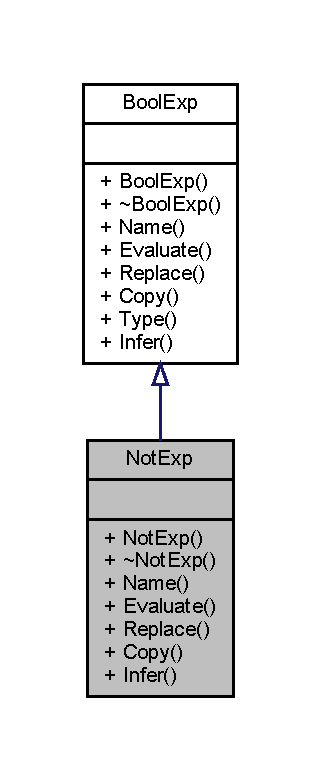
\includegraphics[width=154pt]{classNotExp__inherit__graph}
\end{center}
\end{figure}


Collaboration diagram for Not\+Exp\+:
\nopagebreak
\begin{figure}[H]
\begin{center}
\leavevmode
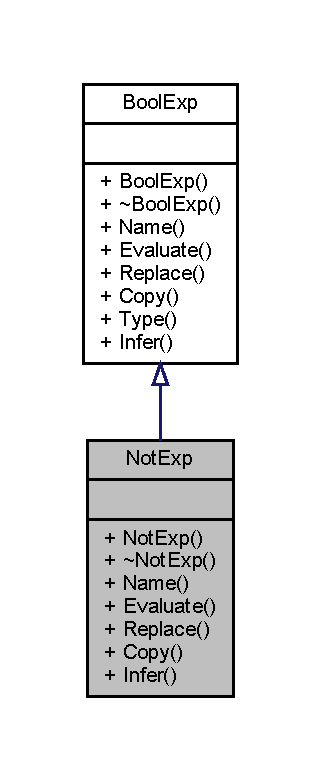
\includegraphics[width=154pt]{classNotExp__coll__graph}
\end{center}
\end{figure}
\subsection*{Public Member Functions}
\begin{DoxyCompactItemize}
\item 
\mbox{\hyperlink{classNotExp_a490e8c258f876cd07a9e6b1eca5d41cc}{Not\+Exp}} (shared\+\_\+ptr$<$ \mbox{\hyperlink{classBoolExp}{Bool\+Exp}} $>$ op)
\item 
virtual \mbox{\hyperlink{classNotExp_ad2533f2e22a5df49eac125d4c5d82936}{$\sim$\+Not\+Exp}} ()
\item 
virtual string \mbox{\hyperlink{classNotExp_a7363cb79787e02ca362a4ea6cdd6d7e2}{Name}} () const
\item 
virtual bool \mbox{\hyperlink{classNotExp_a4bf3ac9a898127b4d0c63db2a5f7a82f}{Evaluate}} (\mbox{\hyperlink{classContext}{Context}} \&con)
\item 
virtual shared\+\_\+ptr$<$ \mbox{\hyperlink{classBoolExp}{Bool\+Exp}} $>$ \mbox{\hyperlink{classNotExp_aeba42c37b59e0eaaf981260e4b163d98}{Replace}} (string, \mbox{\hyperlink{classBoolExp}{Bool\+Exp}} \&)
\item 
virtual shared\+\_\+ptr$<$ \mbox{\hyperlink{classBoolExp}{Bool\+Exp}} $>$ \mbox{\hyperlink{classNotExp_adb36074264fb55186f781680cb6c35f9}{Copy}} () const
\item 
virtual \mbox{\hyperlink{structBoolReturn}{Bool\+Return}} \mbox{\hyperlink{classNotExp_ad7ec5fee6dd934a3db7f72cc9e0b809a}{Infer}} ()
\end{DoxyCompactItemize}


\subsection{Detailed Description}
\mbox{\hyperlink{classNotExp}{Not\+Exp}}\textquotesingle{}s are derived from \mbox{\hyperlink{classBoolExp}{Bool\+Exp}}\textquotesingle{}s they implement the logical proposition $\sim$A note that a \mbox{\hyperlink{classNotExp}{Not\+Exp}} can contain any other kind of \mbox{\hyperlink{classBoolExp}{Bool\+Exp}} ex\+: $\sim$(A\&(B-\/$>$(CvD))) is a valid \mbox{\hyperlink{classNotExp}{Not\+Exp}} 

\subsection{Constructor \& Destructor Documentation}
\mbox{\Hypertarget{classNotExp_a490e8c258f876cd07a9e6b1eca5d41cc}\label{classNotExp_a490e8c258f876cd07a9e6b1eca5d41cc}} 
\index{Not\+Exp@{Not\+Exp}!Not\+Exp@{Not\+Exp}}
\index{Not\+Exp@{Not\+Exp}!Not\+Exp@{Not\+Exp}}
\subsubsection{\texorpdfstring{Not\+Exp()}{NotExp()}}
{\footnotesize\ttfamily Not\+Exp\+::\+Not\+Exp (\begin{DoxyParamCaption}\item[{shared\+\_\+ptr$<$ \mbox{\hyperlink{classBoolExp}{Bool\+Exp}} $>$}]{op }\end{DoxyParamCaption})}

Constructs the specified \mbox{\hyperlink{classNotExp}{Not\+Exp}} 
\begin{DoxyParams}{Parameters}
{\em op} & becomes the operand for this \mbox{\hyperlink{classNotExp}{Not\+Exp}} \\
\hline
\end{DoxyParams}
\mbox{\Hypertarget{classNotExp_ad2533f2e22a5df49eac125d4c5d82936}\label{classNotExp_ad2533f2e22a5df49eac125d4c5d82936}} 
\index{Not\+Exp@{Not\+Exp}!````~Not\+Exp@{$\sim$\+Not\+Exp}}
\index{````~Not\+Exp@{$\sim$\+Not\+Exp}!Not\+Exp@{Not\+Exp}}
\subsubsection{\texorpdfstring{$\sim$\+Not\+Exp()}{~NotExp()}}
{\footnotesize\ttfamily Not\+Exp\+::$\sim$\+Not\+Exp (\begin{DoxyParamCaption}{ }\end{DoxyParamCaption})\hspace{0.3cm}{\ttfamily [virtual]}}

The \mbox{\hyperlink{classNotExp}{Not\+Exp}} destructor 

\subsection{Member Function Documentation}
\mbox{\Hypertarget{classNotExp_adb36074264fb55186f781680cb6c35f9}\label{classNotExp_adb36074264fb55186f781680cb6c35f9}} 
\index{Not\+Exp@{Not\+Exp}!Copy@{Copy}}
\index{Copy@{Copy}!Not\+Exp@{Not\+Exp}}
\subsubsection{\texorpdfstring{Copy()}{Copy()}}
{\footnotesize\ttfamily shared\+\_\+ptr$<$ \mbox{\hyperlink{classBoolExp}{Bool\+Exp}} $>$ Not\+Exp\+::\+Copy (\begin{DoxyParamCaption}{ }\end{DoxyParamCaption}) const\hspace{0.3cm}{\ttfamily [virtual]}}

Create a copy of this \mbox{\hyperlink{classNotExp}{Not\+Exp}} \begin{DoxyReturn}{Returns}
returns the copy of this \mbox{\hyperlink{classNotExp}{Not\+Exp}} 
\end{DoxyReturn}


Implements \mbox{\hyperlink{classBoolExp_a846c30d1730cf645a040978a4cf7cdbb}{Bool\+Exp}}.

\mbox{\Hypertarget{classNotExp_a4bf3ac9a898127b4d0c63db2a5f7a82f}\label{classNotExp_a4bf3ac9a898127b4d0c63db2a5f7a82f}} 
\index{Not\+Exp@{Not\+Exp}!Evaluate@{Evaluate}}
\index{Evaluate@{Evaluate}!Not\+Exp@{Not\+Exp}}
\subsubsection{\texorpdfstring{Evaluate()}{Evaluate()}}
{\footnotesize\ttfamily bool Not\+Exp\+::\+Evaluate (\begin{DoxyParamCaption}\item[{\mbox{\hyperlink{classContext}{Context}} \&}]{con }\end{DoxyParamCaption})\hspace{0.3cm}{\ttfamily [virtual]}}

Recursively evaluates the \mbox{\hyperlink{classNotExp}{Not\+Exp}} via !op1.\mbox{\hyperlink{classNotExp_a4bf3ac9a898127b4d0c63db2a5f7a82f}{Evaluate()}} 
\begin{DoxyParams}{Parameters}
{\em con} & is the \mbox{\hyperlink{classContext}{Context}} class which maps variables to values \\
\hline
\end{DoxyParams}
\begin{DoxyReturn}{Returns}
returns the evaluation of the \mbox{\hyperlink{classBoolExp}{Bool\+Exp}} as a boolean 
\end{DoxyReturn}


Implements \mbox{\hyperlink{classBoolExp_a591fb5f9cb849e0f56e596406a9a10d0}{Bool\+Exp}}.

\mbox{\Hypertarget{classNotExp_ad7ec5fee6dd934a3db7f72cc9e0b809a}\label{classNotExp_ad7ec5fee6dd934a3db7f72cc9e0b809a}} 
\index{Not\+Exp@{Not\+Exp}!Infer@{Infer}}
\index{Infer@{Infer}!Not\+Exp@{Not\+Exp}}
\subsubsection{\texorpdfstring{Infer()}{Infer()}}
{\footnotesize\ttfamily \mbox{\hyperlink{structBoolReturn}{Bool\+Return}} Not\+Exp\+::\+Infer (\begin{DoxyParamCaption}{ }\end{DoxyParamCaption})\hspace{0.3cm}{\ttfamily [virtual]}}

Make an inference from this \mbox{\hyperlink{classNotExp}{Not\+Exp}} \begin{DoxyReturn}{Returns}
returns a \mbox{\hyperlink{structBoolReturn}{Bool\+Return}} with both operands set to the operands of this \mbox{\hyperlink{classNotExp}{Not\+Exp}} 
\end{DoxyReturn}


Implements \mbox{\hyperlink{classBoolExp_a0e5d4a241332ae72d083645e4b71e0e6}{Bool\+Exp}}.

\mbox{\Hypertarget{classNotExp_a7363cb79787e02ca362a4ea6cdd6d7e2}\label{classNotExp_a7363cb79787e02ca362a4ea6cdd6d7e2}} 
\index{Not\+Exp@{Not\+Exp}!Name@{Name}}
\index{Name@{Name}!Not\+Exp@{Not\+Exp}}
\subsubsection{\texorpdfstring{Name()}{Name()}}
{\footnotesize\ttfamily string Not\+Exp\+::\+Name (\begin{DoxyParamCaption}{ }\end{DoxyParamCaption}) const\hspace{0.3cm}{\ttfamily [virtual]}}

Recursively retrieves and returns a string representation of the \mbox{\hyperlink{classNotExp}{Not\+Exp}} \begin{DoxyReturn}{Returns}
returns the name of this \mbox{\hyperlink{classNotExp}{Not\+Exp}} as a string 
\end{DoxyReturn}


Implements \mbox{\hyperlink{classBoolExp_a3fdb64a9b8fd54e33d755ff4a577d11a}{Bool\+Exp}}.

\mbox{\Hypertarget{classNotExp_aeba42c37b59e0eaaf981260e4b163d98}\label{classNotExp_aeba42c37b59e0eaaf981260e4b163d98}} 
\index{Not\+Exp@{Not\+Exp}!Replace@{Replace}}
\index{Replace@{Replace}!Not\+Exp@{Not\+Exp}}
\subsubsection{\texorpdfstring{Replace()}{Replace()}}
{\footnotesize\ttfamily shared\+\_\+ptr$<$ \mbox{\hyperlink{classBoolExp}{Bool\+Exp}} $>$ Not\+Exp\+::\+Replace (\begin{DoxyParamCaption}\item[{string}]{name,  }\item[{\mbox{\hyperlink{classBoolExp}{Bool\+Exp}} \&}]{exp }\end{DoxyParamCaption})\hspace{0.3cm}{\ttfamily [virtual]}}

Left in for possible future usage see \mbox{\hyperlink{classBoolExp}{Bool\+Exp}} explanation 
\begin{DoxyParams}{Parameters}
{\em name} & the name to use for replacement \\
\hline
{\em exp} & the expression to use for replacement \\
\hline
\end{DoxyParams}
\begin{DoxyReturn}{Returns}
returns the new \mbox{\hyperlink{classBoolExp}{Bool\+Exp}} 
\end{DoxyReturn}


Implements \mbox{\hyperlink{classBoolExp_a6448b7121c238759cc9cc8e48d6f8773}{Bool\+Exp}}.



The documentation for this class was generated from the following files\+:\begin{DoxyCompactItemize}
\item 
\mbox{\hyperlink{notexp_8h}{notexp.\+h}}\item 
\mbox{\hyperlink{notexp_8cpp}{notexp.\+cpp}}\end{DoxyCompactItemize}

\hypertarget{classOrExp}{}\section{Or\+Exp Class Reference}
\label{classOrExp}\index{Or\+Exp@{Or\+Exp}}


{\ttfamily \#include $<$orexp.\+h$>$}



Inheritance diagram for Or\+Exp\+:
\nopagebreak
\begin{figure}[H]
\begin{center}
\leavevmode
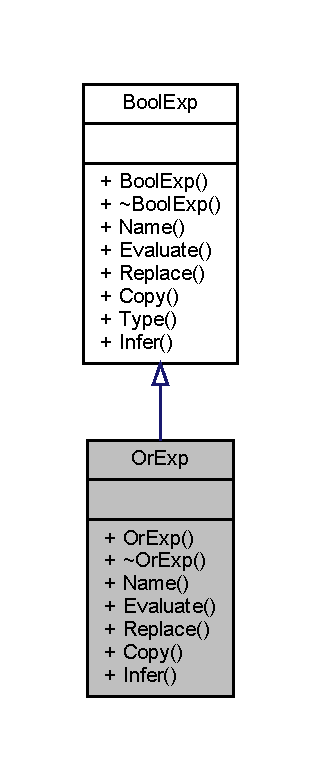
\includegraphics[width=154pt]{classOrExp__inherit__graph}
\end{center}
\end{figure}


Collaboration diagram for Or\+Exp\+:
\nopagebreak
\begin{figure}[H]
\begin{center}
\leavevmode
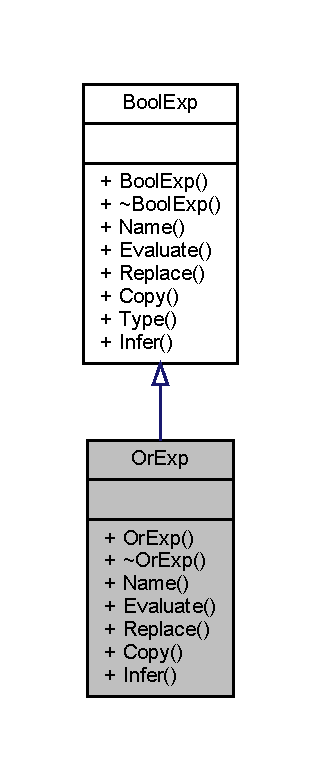
\includegraphics[width=154pt]{classOrExp__coll__graph}
\end{center}
\end{figure}
\subsection*{Public Member Functions}
\begin{DoxyCompactItemize}
\item 
\mbox{\hyperlink{classOrExp_a600a2b33932bd7e8ea4011180a9ae791}{Or\+Exp}} (shared\+\_\+ptr$<$ \mbox{\hyperlink{classBoolExp}{Bool\+Exp}} $>$, shared\+\_\+ptr$<$ \mbox{\hyperlink{classBoolExp}{Bool\+Exp}} $>$)
\item 
virtual \mbox{\hyperlink{classOrExp_a13e824ccc65f06421b506a3428d73ca5}{$\sim$\+Or\+Exp}} ()
\item 
virtual string \mbox{\hyperlink{classOrExp_a8e535ae2da801bf5a4e8c9fbf3426a8b}{Name}} () const
\item 
virtual bool \mbox{\hyperlink{classOrExp_a2056a325b87621e2a3d0afff79c4163e}{Evaluate}} (\mbox{\hyperlink{classContext}{Context}} \&)
\item 
virtual shared\+\_\+ptr$<$ \mbox{\hyperlink{classBoolExp}{Bool\+Exp}} $>$ \mbox{\hyperlink{classOrExp_a256171f2cf3d3165745d6df9390d9ab7}{Replace}} (string, \mbox{\hyperlink{classBoolExp}{Bool\+Exp}} \&)
\item 
virtual shared\+\_\+ptr$<$ \mbox{\hyperlink{classBoolExp}{Bool\+Exp}} $>$ \mbox{\hyperlink{classOrExp_a142f557d9b95c4464dbd9167dbb9fe51}{Copy}} () const
\item 
virtual \mbox{\hyperlink{structBoolReturn}{Bool\+Return}} \mbox{\hyperlink{classOrExp_aa3b98be68c00bc0c43a9eec5a47cdec9}{Infer}} ()
\end{DoxyCompactItemize}


\subsection{Detailed Description}
\mbox{\hyperlink{classOrExp}{Or\+Exp}}\textquotesingle{}s are derived from \mbox{\hyperlink{classBoolExp}{Bool\+Exp}}\textquotesingle{}s they implement the logical proposition (AvB) 

\subsection{Constructor \& Destructor Documentation}
\mbox{\Hypertarget{classOrExp_a600a2b33932bd7e8ea4011180a9ae791}\label{classOrExp_a600a2b33932bd7e8ea4011180a9ae791}} 
\index{Or\+Exp@{Or\+Exp}!Or\+Exp@{Or\+Exp}}
\index{Or\+Exp@{Or\+Exp}!Or\+Exp@{Or\+Exp}}
\subsubsection{\texorpdfstring{Or\+Exp()}{OrExp()}}
{\footnotesize\ttfamily Or\+Exp\+::\+Or\+Exp (\begin{DoxyParamCaption}\item[{shared\+\_\+ptr$<$ \mbox{\hyperlink{classBoolExp}{Bool\+Exp}} $>$}]{op1,  }\item[{shared\+\_\+ptr$<$ \mbox{\hyperlink{classBoolExp}{Bool\+Exp}} $>$}]{op2 }\end{DoxyParamCaption})}

Constructs the specified \mbox{\hyperlink{classOrExp}{Or\+Exp}} 
\begin{DoxyParams}{Parameters}
{\em op1} & becomes the left hand operand \\
\hline
{\em op2} & becomes the right hand operand \\
\hline
\end{DoxyParams}
\mbox{\Hypertarget{classOrExp_a13e824ccc65f06421b506a3428d73ca5}\label{classOrExp_a13e824ccc65f06421b506a3428d73ca5}} 
\index{Or\+Exp@{Or\+Exp}!````~Or\+Exp@{$\sim$\+Or\+Exp}}
\index{````~Or\+Exp@{$\sim$\+Or\+Exp}!Or\+Exp@{Or\+Exp}}
\subsubsection{\texorpdfstring{$\sim$\+Or\+Exp()}{~OrExp()}}
{\footnotesize\ttfamily Or\+Exp\+::$\sim$\+Or\+Exp (\begin{DoxyParamCaption}{ }\end{DoxyParamCaption})\hspace{0.3cm}{\ttfamily [virtual]}}

The \mbox{\hyperlink{classOrExp}{Or\+Exp}} destructor 

\subsection{Member Function Documentation}
\mbox{\Hypertarget{classOrExp_a142f557d9b95c4464dbd9167dbb9fe51}\label{classOrExp_a142f557d9b95c4464dbd9167dbb9fe51}} 
\index{Or\+Exp@{Or\+Exp}!Copy@{Copy}}
\index{Copy@{Copy}!Or\+Exp@{Or\+Exp}}
\subsubsection{\texorpdfstring{Copy()}{Copy()}}
{\footnotesize\ttfamily shared\+\_\+ptr$<$ \mbox{\hyperlink{classBoolExp}{Bool\+Exp}} $>$ Or\+Exp\+::\+Copy (\begin{DoxyParamCaption}{ }\end{DoxyParamCaption}) const\hspace{0.3cm}{\ttfamily [virtual]}}

Create a copy of this \mbox{\hyperlink{classOrExp}{Or\+Exp}} \begin{DoxyReturn}{Returns}
returns the copy of this \mbox{\hyperlink{classOrExp}{Or\+Exp}} 
\end{DoxyReturn}


Implements \mbox{\hyperlink{classBoolExp_a846c30d1730cf645a040978a4cf7cdbb}{Bool\+Exp}}.

\mbox{\Hypertarget{classOrExp_a2056a325b87621e2a3d0afff79c4163e}\label{classOrExp_a2056a325b87621e2a3d0afff79c4163e}} 
\index{Or\+Exp@{Or\+Exp}!Evaluate@{Evaluate}}
\index{Evaluate@{Evaluate}!Or\+Exp@{Or\+Exp}}
\subsubsection{\texorpdfstring{Evaluate()}{Evaluate()}}
{\footnotesize\ttfamily bool Or\+Exp\+::\+Evaluate (\begin{DoxyParamCaption}\item[{\mbox{\hyperlink{classContext}{Context}} \&}]{con }\end{DoxyParamCaption})\hspace{0.3cm}{\ttfamily [virtual]}}

Recursively evaluates the \mbox{\hyperlink{classOrExp}{Or\+Exp}} via (op1.\+Evaluate() $\vert$$\vert$ op2.\+Evaluate()) 
\begin{DoxyParams}{Parameters}
{\em con} & is the \mbox{\hyperlink{classContext}{Context}} class which maps variables to values \\
\hline
\end{DoxyParams}
\begin{DoxyReturn}{Returns}
returns the evaluation of the \mbox{\hyperlink{classBoolExp}{Bool\+Exp}} as a boolean 
\end{DoxyReturn}


Implements \mbox{\hyperlink{classBoolExp_a591fb5f9cb849e0f56e596406a9a10d0}{Bool\+Exp}}.

\mbox{\Hypertarget{classOrExp_aa3b98be68c00bc0c43a9eec5a47cdec9}\label{classOrExp_aa3b98be68c00bc0c43a9eec5a47cdec9}} 
\index{Or\+Exp@{Or\+Exp}!Infer@{Infer}}
\index{Infer@{Infer}!Or\+Exp@{Or\+Exp}}
\subsubsection{\texorpdfstring{Infer()}{Infer()}}
{\footnotesize\ttfamily \mbox{\hyperlink{structBoolReturn}{Bool\+Return}} Or\+Exp\+::\+Infer (\begin{DoxyParamCaption}{ }\end{DoxyParamCaption})\hspace{0.3cm}{\ttfamily [virtual]}}

Make an inference from this \mbox{\hyperlink{classOrExp}{Or\+Exp}} \begin{DoxyReturn}{Returns}
returns a \mbox{\hyperlink{structBoolReturn}{Bool\+Return}} with both operands set to the operands of this \mbox{\hyperlink{classOrExp}{Or\+Exp}} 
\end{DoxyReturn}


Implements \mbox{\hyperlink{classBoolExp_a0e5d4a241332ae72d083645e4b71e0e6}{Bool\+Exp}}.

\mbox{\Hypertarget{classOrExp_a8e535ae2da801bf5a4e8c9fbf3426a8b}\label{classOrExp_a8e535ae2da801bf5a4e8c9fbf3426a8b}} 
\index{Or\+Exp@{Or\+Exp}!Name@{Name}}
\index{Name@{Name}!Or\+Exp@{Or\+Exp}}
\subsubsection{\texorpdfstring{Name()}{Name()}}
{\footnotesize\ttfamily string Or\+Exp\+::\+Name (\begin{DoxyParamCaption}{ }\end{DoxyParamCaption}) const\hspace{0.3cm}{\ttfamily [virtual]}}

Recursively retrieves and returns a string representation of the \mbox{\hyperlink{classOrExp}{Or\+Exp}} \begin{DoxyReturn}{Returns}
returns the name of this \mbox{\hyperlink{classOrExp}{Or\+Exp}} as a string 
\end{DoxyReturn}


Implements \mbox{\hyperlink{classBoolExp_a3fdb64a9b8fd54e33d755ff4a577d11a}{Bool\+Exp}}.

\mbox{\Hypertarget{classOrExp_a256171f2cf3d3165745d6df9390d9ab7}\label{classOrExp_a256171f2cf3d3165745d6df9390d9ab7}} 
\index{Or\+Exp@{Or\+Exp}!Replace@{Replace}}
\index{Replace@{Replace}!Or\+Exp@{Or\+Exp}}
\subsubsection{\texorpdfstring{Replace()}{Replace()}}
{\footnotesize\ttfamily shared\+\_\+ptr$<$ \mbox{\hyperlink{classBoolExp}{Bool\+Exp}} $>$ Or\+Exp\+::\+Replace (\begin{DoxyParamCaption}\item[{string}]{name,  }\item[{\mbox{\hyperlink{classBoolExp}{Bool\+Exp}} \&}]{exp }\end{DoxyParamCaption})\hspace{0.3cm}{\ttfamily [virtual]}}

Left in for possible future usage see \mbox{\hyperlink{classBoolExp}{Bool\+Exp}} explanation 
\begin{DoxyParams}{Parameters}
{\em name} & the name to use for replacement \\
\hline
{\em exp} & the expression to use for replacement \\
\hline
\end{DoxyParams}
\begin{DoxyReturn}{Returns}
returns the new \mbox{\hyperlink{classBoolExp}{Bool\+Exp}} 
\end{DoxyReturn}


Implements \mbox{\hyperlink{classBoolExp_a6448b7121c238759cc9cc8e48d6f8773}{Bool\+Exp}}.



The documentation for this class was generated from the following files\+:\begin{DoxyCompactItemize}
\item 
\mbox{\hyperlink{orexp_8h}{orexp.\+h}}\item 
\mbox{\hyperlink{orexp_8cpp}{orexp.\+cpp}}\end{DoxyCompactItemize}

\hypertarget{classProver}{}\section{Prover Class Reference}
\label{classProver}\index{Prover@{Prover}}


{\ttfamily \#include $<$prover.\+h$>$}



Collaboration diagram for Prover\+:
\nopagebreak
\begin{figure}[H]
\begin{center}
\leavevmode
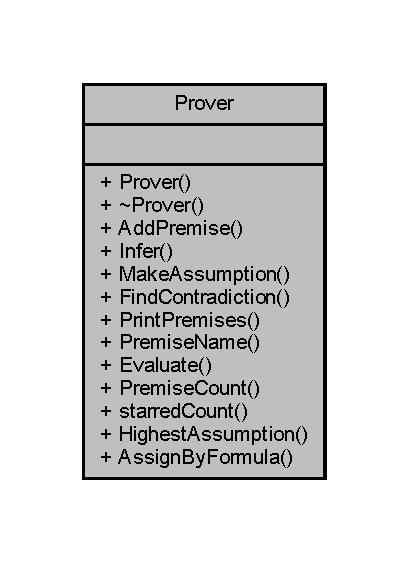
\includegraphics[width=196pt]{classProver__coll__graph}
\end{center}
\end{figure}
\subsection*{Public Member Functions}
\begin{DoxyCompactItemize}
\item 
\mbox{\hyperlink{classProver_a53e01b8533298b61a5b7f7abf641df32}{Prover}} ()
\item 
\mbox{\hyperlink{classProver_a3bf49b1519cdec0eca3c22ebfe23fbde}{$\sim$\+Prover}} ()
\item 
void \mbox{\hyperlink{classProver_aa861628e3d89e9cd634b18aaacc99e58}{Add\+Premise}} (shared\+\_\+ptr$<$ \mbox{\hyperlink{classBoolExp}{Bool\+Exp}} $>$ exp, \mbox{\hyperlink{boolexp_8h_ac6a79184a0a7c1d2e3ea745512aa2d0c}{Prop\+Type}} p, string reason)
\item 
void \mbox{\hyperlink{classProver_a40376d5e8cc820b45b073dcc9320ed36}{Infer}} (const int i)
\item 
bool \mbox{\hyperlink{classProver_a046549fd07af6d0315a1d0df93215c60}{Make\+Assumption}} ()
\item 
bool \mbox{\hyperlink{classProver_a347682708b1a198c35d7609022ce4dd9}{Find\+Contradiction}} ()
\item 
void \mbox{\hyperlink{classProver_aecc46e8d5521ff62e283755fb44b68e2}{Print\+Premises}} () const
\item 
string \mbox{\hyperlink{classProver_aaf06243b77406aa09ff55e59eec448f3}{Premise\+Name}} (int i) const
\item 
bool \mbox{\hyperlink{classProver_af58f19171272472ab438b144e942c0dd}{Evaluate}} (int i, \mbox{\hyperlink{classContext}{Context}} \&context) const
\item 
int \mbox{\hyperlink{classProver_ab33b18bf4e9c3ea6a3dd48e47e90e5ef}{Premise\+Count}} () const
\item 
int \mbox{\hyperlink{classProver_a21743acd96dd9b8bf26ee02ea8761d88}{starred\+Count}} () const
\item 
int \mbox{\hyperlink{classProver_a98c85ede3242c56e7f7e7f3b42bbd191}{Highest\+Assumption}} () const
\item 
void \mbox{\hyperlink{classProver_a3d4b890f7c8eefb9788e4bd545ea0c0e}{Assign\+By\+Formula}} (\mbox{\hyperlink{classContext}{Context}} \&context)
\end{DoxyCompactItemize}


\subsection{Detailed Description}
One view of proofs stipulates that a proof is an array of well formed propositions generated by various inference rules leading to some concluding formula in this sense a prover is a class containing an array/vector of propositions, bookkeeping metadata and methods for manipulating them. The particular method of proof being implemented is proof by contradiction 

\subsection{Constructor \& Destructor Documentation}
\mbox{\Hypertarget{classProver_a53e01b8533298b61a5b7f7abf641df32}\label{classProver_a53e01b8533298b61a5b7f7abf641df32}} 
\index{Prover@{Prover}!Prover@{Prover}}
\index{Prover@{Prover}!Prover@{Prover}}
\subsubsection{\texorpdfstring{Prover()}{Prover()}}
{\footnotesize\ttfamily Prover\+::\+Prover (\begin{DoxyParamCaption}{ }\end{DoxyParamCaption})}

The prover constructor init \+\_\+prem to 0 and \+\_\+highestasm to 1 \mbox{\Hypertarget{classProver_a3bf49b1519cdec0eca3c22ebfe23fbde}\label{classProver_a3bf49b1519cdec0eca3c22ebfe23fbde}} 
\index{Prover@{Prover}!````~Prover@{$\sim$\+Prover}}
\index{````~Prover@{$\sim$\+Prover}!Prover@{Prover}}
\subsubsection{\texorpdfstring{$\sim$\+Prover()}{~Prover()}}
{\footnotesize\ttfamily Prover\+::$\sim$\+Prover (\begin{DoxyParamCaption}{ }\end{DoxyParamCaption})}

The prover destructor 

\subsection{Member Function Documentation}
\mbox{\Hypertarget{classProver_aa861628e3d89e9cd634b18aaacc99e58}\label{classProver_aa861628e3d89e9cd634b18aaacc99e58}} 
\index{Prover@{Prover}!Add\+Premise@{Add\+Premise}}
\index{Add\+Premise@{Add\+Premise}!Prover@{Prover}}
\subsubsection{\texorpdfstring{Add\+Premise()}{AddPremise()}}
{\footnotesize\ttfamily void Prover\+::\+Add\+Premise (\begin{DoxyParamCaption}\item[{shared\+\_\+ptr$<$ \mbox{\hyperlink{classBoolExp}{Bool\+Exp}} $>$}]{exp,  }\item[{\mbox{\hyperlink{boolexp_8h_ac6a79184a0a7c1d2e3ea745512aa2d0c}{Prop\+Type}}}]{p,  }\item[{string}]{reason }\end{DoxyParamCaption})}

add the premise exp of type p because of reason 
\begin{DoxyParams}{Parameters}
{\em exp} & the expression to add to the proof \\
\hline
{\em p} & the type of expression being added \\
\hline
{\em reason} & the reason for adding the expression \\
\hline
\end{DoxyParams}
\mbox{\Hypertarget{classProver_a3d4b890f7c8eefb9788e4bd545ea0c0e}\label{classProver_a3d4b890f7c8eefb9788e4bd545ea0c0e}} 
\index{Prover@{Prover}!Assign\+By\+Formula@{Assign\+By\+Formula}}
\index{Assign\+By\+Formula@{Assign\+By\+Formula}!Prover@{Prover}}
\subsubsection{\texorpdfstring{Assign\+By\+Formula()}{AssignByFormula()}}
{\footnotesize\ttfamily void Prover\+::\+Assign\+By\+Formula (\begin{DoxyParamCaption}\item[{\mbox{\hyperlink{classContext}{Context}} \&}]{context }\end{DoxyParamCaption})}

Assigns boolean values by formula within the proof from 0 to n and within each formula from left to right 
\begin{DoxyParams}{Parameters}
{\em context} & the context containing the formulas receiving values \\
\hline
\end{DoxyParams}
\mbox{\Hypertarget{classProver_af58f19171272472ab438b144e942c0dd}\label{classProver_af58f19171272472ab438b144e942c0dd}} 
\index{Prover@{Prover}!Evaluate@{Evaluate}}
\index{Evaluate@{Evaluate}!Prover@{Prover}}
\subsubsection{\texorpdfstring{Evaluate()}{Evaluate()}}
{\footnotesize\ttfamily bool Prover\+::\+Evaluate (\begin{DoxyParamCaption}\item[{int}]{i,  }\item[{\mbox{\hyperlink{classContext}{Context}} \&}]{context }\end{DoxyParamCaption}) const}

evaluate the premise at index i given the input \mbox{\hyperlink{classContext}{Context}} map 
\begin{DoxyParams}{Parameters}
{\em i} & the index of the formula to be evaluated \\
\hline
{\em context} & the context mapping variables to boolean values \\
\hline
\end{DoxyParams}
\begin{DoxyReturn}{Returns}
returns the evaluation of the formula at index i under the given context 
\end{DoxyReturn}
\mbox{\Hypertarget{classProver_a347682708b1a198c35d7609022ce4dd9}\label{classProver_a347682708b1a198c35d7609022ce4dd9}} 
\index{Prover@{Prover}!Find\+Contradiction@{Find\+Contradiction}}
\index{Find\+Contradiction@{Find\+Contradiction}!Prover@{Prover}}
\subsubsection{\texorpdfstring{Find\+Contradiction()}{FindContradiction()}}
{\footnotesize\ttfamily bool Prover\+::\+Find\+Contradiction (\begin{DoxyParamCaption}{ }\end{DoxyParamCaption})}

scan the whole proof attempt to find at least one contradiction if one is found block off all formulas at matching assumption levels \begin{DoxyReturn}{Returns}
returns true if a contradiction was found returns false if a contradiction is not found 
\end{DoxyReturn}
\mbox{\Hypertarget{classProver_a98c85ede3242c56e7f7e7f3b42bbd191}\label{classProver_a98c85ede3242c56e7f7e7f3b42bbd191}} 
\index{Prover@{Prover}!Highest\+Assumption@{Highest\+Assumption}}
\index{Highest\+Assumption@{Highest\+Assumption}!Prover@{Prover}}
\subsubsection{\texorpdfstring{Highest\+Assumption()}{HighestAssumption()}}
{\footnotesize\ttfamily int Prover\+::\+Highest\+Assumption (\begin{DoxyParamCaption}{ }\end{DoxyParamCaption}) const}

returns the current highest assumption level in the proof 
\begin{DoxyParams}{Parameters}
{\em returns} & the highest assumption level so far in the proof \\
\hline
\end{DoxyParams}
\mbox{\Hypertarget{classProver_a40376d5e8cc820b45b073dcc9320ed36}\label{classProver_a40376d5e8cc820b45b073dcc9320ed36}} 
\index{Prover@{Prover}!Infer@{Infer}}
\index{Infer@{Infer}!Prover@{Prover}}
\subsubsection{\texorpdfstring{Infer()}{Infer()}}
{\footnotesize\ttfamily void Prover\+::\+Infer (\begin{DoxyParamCaption}\item[{const int}]{i }\end{DoxyParamCaption})}

attempt to make an inference off of the formula at index i \mbox{\Hypertarget{classProver_a046549fd07af6d0315a1d0df93215c60}\label{classProver_a046549fd07af6d0315a1d0df93215c60}} 
\index{Prover@{Prover}!Make\+Assumption@{Make\+Assumption}}
\index{Make\+Assumption@{Make\+Assumption}!Prover@{Prover}}
\subsubsection{\texorpdfstring{Make\+Assumption()}{MakeAssumption()}}
{\footnotesize\ttfamily bool Prover\+::\+Make\+Assumption (\begin{DoxyParamCaption}{ }\end{DoxyParamCaption})}

scan the whole proof and attemp to make a single assumption \begin{DoxyReturn}{Returns}
returns true if an assumption is made returns false if no assumption is made 
\end{DoxyReturn}
\mbox{\Hypertarget{classProver_ab33b18bf4e9c3ea6a3dd48e47e90e5ef}\label{classProver_ab33b18bf4e9c3ea6a3dd48e47e90e5ef}} 
\index{Prover@{Prover}!Premise\+Count@{Premise\+Count}}
\index{Premise\+Count@{Premise\+Count}!Prover@{Prover}}
\subsubsection{\texorpdfstring{Premise\+Count()}{PremiseCount()}}
{\footnotesize\ttfamily int Prover\+::\+Premise\+Count (\begin{DoxyParamCaption}{ }\end{DoxyParamCaption}) const}

return the count of premises in the proof \begin{DoxyReturn}{Returns}
returns how many premises in the proof 
\end{DoxyReturn}
\mbox{\Hypertarget{classProver_aaf06243b77406aa09ff55e59eec448f3}\label{classProver_aaf06243b77406aa09ff55e59eec448f3}} 
\index{Prover@{Prover}!Premise\+Name@{Premise\+Name}}
\index{Premise\+Name@{Premise\+Name}!Prover@{Prover}}
\subsubsection{\texorpdfstring{Premise\+Name()}{PremiseName()}}
{\footnotesize\ttfamily string Prover\+::\+Premise\+Name (\begin{DoxyParamCaption}\item[{int}]{i }\end{DoxyParamCaption}) const}

return the string form of the premise at index i 
\begin{DoxyParams}{Parameters}
{\em i} & the index of the formula being referred to \\
\hline
\end{DoxyParams}
\begin{DoxyReturn}{Returns}
returns the string at index i 
\end{DoxyReturn}
\mbox{\Hypertarget{classProver_aecc46e8d5521ff62e283755fb44b68e2}\label{classProver_aecc46e8d5521ff62e283755fb44b68e2}} 
\index{Prover@{Prover}!Print\+Premises@{Print\+Premises}}
\index{Print\+Premises@{Print\+Premises}!Prover@{Prover}}
\subsubsection{\texorpdfstring{Print\+Premises()}{PrintPremises()}}
{\footnotesize\ttfamily void Prover\+::\+Print\+Premises (\begin{DoxyParamCaption}{ }\end{DoxyParamCaption}) const}

print the current state of the proof include all assumption starred blocked info and reasons \mbox{\Hypertarget{classProver_a21743acd96dd9b8bf26ee02ea8761d88}\label{classProver_a21743acd96dd9b8bf26ee02ea8761d88}} 
\index{Prover@{Prover}!starred\+Count@{starred\+Count}}
\index{starred\+Count@{starred\+Count}!Prover@{Prover}}
\subsubsection{\texorpdfstring{starred\+Count()}{starredCount()}}
{\footnotesize\ttfamily int Prover\+::starred\+Count (\begin{DoxyParamCaption}{ }\end{DoxyParamCaption}) const}

return how many formulas are starred in the proof \begin{DoxyReturn}{Returns}
returns the count of formulas that have been starred thus far in the proof 
\end{DoxyReturn}


The documentation for this class was generated from the following files\+:\begin{DoxyCompactItemize}
\item 
\mbox{\hyperlink{prover_8h}{prover.\+h}}\item 
\mbox{\hyperlink{prover_8cpp}{prover.\+cpp}}\end{DoxyCompactItemize}

\hypertarget{classVarExp}{}\section{Var\+Exp Class Reference}
\label{classVarExp}\index{Var\+Exp@{Var\+Exp}}


{\ttfamily \#include $<$varexp.\+h$>$}



Inheritance diagram for Var\+Exp\+:
\nopagebreak
\begin{figure}[H]
\begin{center}
\leavevmode
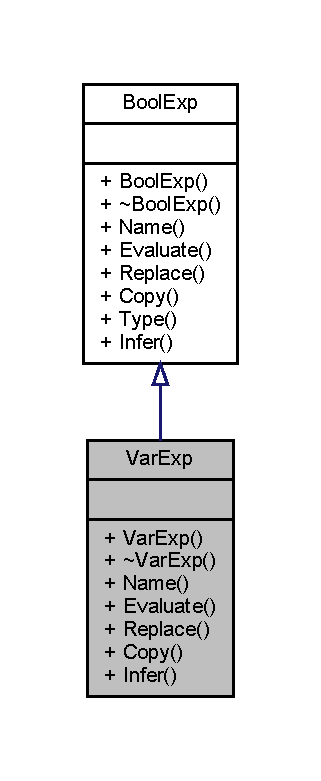
\includegraphics[width=154pt]{classVarExp__inherit__graph}
\end{center}
\end{figure}


Collaboration diagram for Var\+Exp\+:
\nopagebreak
\begin{figure}[H]
\begin{center}
\leavevmode
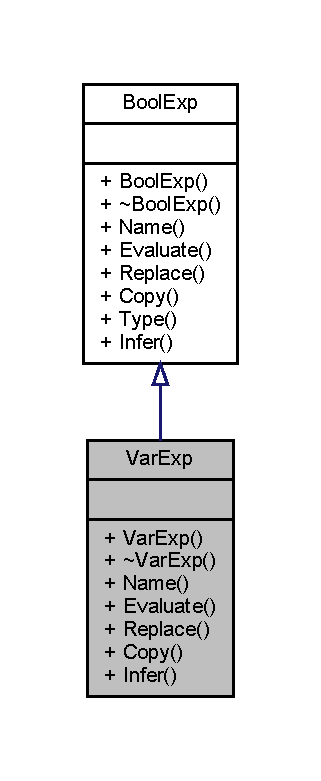
\includegraphics[width=154pt]{classVarExp__coll__graph}
\end{center}
\end{figure}
\subsection*{Public Member Functions}
\begin{DoxyCompactItemize}
\item 
\mbox{\hyperlink{classVarExp_a8281aeafbde537140bacfed1a894e889}{Var\+Exp}} (string)
\item 
virtual \mbox{\hyperlink{classVarExp_a5e1198cc9abe533d0a606e27d7b20e75}{$\sim$\+Var\+Exp}} ()
\item 
virtual string \mbox{\hyperlink{classVarExp_af50f77454d193ebfd7633f5f20becaf4}{Name}} () const
\item 
virtual bool \mbox{\hyperlink{classVarExp_af9d73e76a255123e00d5ebb1ae703188}{Evaluate}} (\mbox{\hyperlink{classContext}{Context}} \&con)
\item 
virtual shared\+\_\+ptr$<$ \mbox{\hyperlink{classBoolExp}{Bool\+Exp}} $>$ \mbox{\hyperlink{classVarExp_a0b716a76069a7fad3b99b86a9bd9d331}{Replace}} (string, \mbox{\hyperlink{classBoolExp}{Bool\+Exp}} \&)
\item 
virtual shared\+\_\+ptr$<$ \mbox{\hyperlink{classBoolExp}{Bool\+Exp}} $>$ \mbox{\hyperlink{classVarExp_ad93ffa6aa927bc41c9765bc37b4d0a63}{Copy}} () const
\item 
virtual \mbox{\hyperlink{structBoolReturn}{Bool\+Return}} \mbox{\hyperlink{classVarExp_a6c3e1736ade0456d23085923bc3fef61}{Infer}} ()
\end{DoxyCompactItemize}


\subsection{Detailed Description}
\mbox{\hyperlink{classVarExp}{Var\+Exp}} are just names they can be thought of as terminals in the language of propositional formulas 

\subsection{Constructor \& Destructor Documentation}
\mbox{\Hypertarget{classVarExp_a8281aeafbde537140bacfed1a894e889}\label{classVarExp_a8281aeafbde537140bacfed1a894e889}} 
\index{Var\+Exp@{Var\+Exp}!Var\+Exp@{Var\+Exp}}
\index{Var\+Exp@{Var\+Exp}!Var\+Exp@{Var\+Exp}}
\subsubsection{\texorpdfstring{Var\+Exp()}{VarExp()}}
{\footnotesize\ttfamily Var\+Exp\+::\+Var\+Exp (\begin{DoxyParamCaption}\item[{string}]{nm }\end{DoxyParamCaption})}

Var\+Exps can be constructed via passing the intended name \mbox{\Hypertarget{classVarExp_a5e1198cc9abe533d0a606e27d7b20e75}\label{classVarExp_a5e1198cc9abe533d0a606e27d7b20e75}} 
\index{Var\+Exp@{Var\+Exp}!````~Var\+Exp@{$\sim$\+Var\+Exp}}
\index{````~Var\+Exp@{$\sim$\+Var\+Exp}!Var\+Exp@{Var\+Exp}}
\subsubsection{\texorpdfstring{$\sim$\+Var\+Exp()}{~VarExp()}}
{\footnotesize\ttfamily Var\+Exp\+::$\sim$\+Var\+Exp (\begin{DoxyParamCaption}{ }\end{DoxyParamCaption})\hspace{0.3cm}{\ttfamily [virtual]}}



\subsection{Member Function Documentation}
\mbox{\Hypertarget{classVarExp_ad93ffa6aa927bc41c9765bc37b4d0a63}\label{classVarExp_ad93ffa6aa927bc41c9765bc37b4d0a63}} 
\index{Var\+Exp@{Var\+Exp}!Copy@{Copy}}
\index{Copy@{Copy}!Var\+Exp@{Var\+Exp}}
\subsubsection{\texorpdfstring{Copy()}{Copy()}}
{\footnotesize\ttfamily shared\+\_\+ptr$<$ \mbox{\hyperlink{classBoolExp}{Bool\+Exp}} $>$ Var\+Exp\+::\+Copy (\begin{DoxyParamCaption}{ }\end{DoxyParamCaption}) const\hspace{0.3cm}{\ttfamily [virtual]}}

Create a copy of this \mbox{\hyperlink{classVarExp}{Var\+Exp}} \begin{DoxyReturn}{Returns}
returns the copy of this \mbox{\hyperlink{classVarExp}{Var\+Exp}} 
\end{DoxyReturn}


Implements \mbox{\hyperlink{classBoolExp_a846c30d1730cf645a040978a4cf7cdbb}{Bool\+Exp}}.

\mbox{\Hypertarget{classVarExp_af9d73e76a255123e00d5ebb1ae703188}\label{classVarExp_af9d73e76a255123e00d5ebb1ae703188}} 
\index{Var\+Exp@{Var\+Exp}!Evaluate@{Evaluate}}
\index{Evaluate@{Evaluate}!Var\+Exp@{Var\+Exp}}
\subsubsection{\texorpdfstring{Evaluate()}{Evaluate()}}
{\footnotesize\ttfamily bool Var\+Exp\+::\+Evaluate (\begin{DoxyParamCaption}\item[{\mbox{\hyperlink{classContext}{Context}} \&}]{con }\end{DoxyParamCaption})\hspace{0.3cm}{\ttfamily [virtual]}}

Lookups the name of this \mbox{\hyperlink{classVarExp}{Var\+Exp}} in context and returns its value 
\begin{DoxyParams}{Parameters}
{\em con} & the context for name lookup to be used on \\
\hline
\end{DoxyParams}
\begin{DoxyReturn}{Returns}
returns the evaluation of the \mbox{\hyperlink{classBoolExp}{Bool\+Exp}} as a boolean 
\end{DoxyReturn}


Implements \mbox{\hyperlink{classBoolExp_a591fb5f9cb849e0f56e596406a9a10d0}{Bool\+Exp}}.

\mbox{\Hypertarget{classVarExp_a6c3e1736ade0456d23085923bc3fef61}\label{classVarExp_a6c3e1736ade0456d23085923bc3fef61}} 
\index{Var\+Exp@{Var\+Exp}!Infer@{Infer}}
\index{Infer@{Infer}!Var\+Exp@{Var\+Exp}}
\subsubsection{\texorpdfstring{Infer()}{Infer()}}
{\footnotesize\ttfamily \mbox{\hyperlink{structBoolReturn}{Bool\+Return}} Var\+Exp\+::\+Infer (\begin{DoxyParamCaption}{ }\end{DoxyParamCaption})\hspace{0.3cm}{\ttfamily [virtual]}}

returns a \mbox{\hyperlink{structBoolReturn}{Bool\+Return}} containing two of the same \mbox{\hyperlink{classVarExp}{Var\+Exp}}\textquotesingle{}s \begin{DoxyReturn}{Returns}
returns a \mbox{\hyperlink{structBoolReturn}{Bool\+Return}} with operands as copies of this \mbox{\hyperlink{classVarExp}{Var\+Exp}} 
\end{DoxyReturn}


Implements \mbox{\hyperlink{classBoolExp_a0e5d4a241332ae72d083645e4b71e0e6}{Bool\+Exp}}.

\mbox{\Hypertarget{classVarExp_af50f77454d193ebfd7633f5f20becaf4}\label{classVarExp_af50f77454d193ebfd7633f5f20becaf4}} 
\index{Var\+Exp@{Var\+Exp}!Name@{Name}}
\index{Name@{Name}!Var\+Exp@{Var\+Exp}}
\subsubsection{\texorpdfstring{Name()}{Name()}}
{\footnotesize\ttfamily string Var\+Exp\+::\+Name (\begin{DoxyParamCaption}{ }\end{DoxyParamCaption}) const\hspace{0.3cm}{\ttfamily [virtual]}}

Recursively retrieves and returns a string representation of the \mbox{\hyperlink{classVarExp}{Var\+Exp}} \begin{DoxyReturn}{Returns}
returns the name of this \mbox{\hyperlink{classVarExp}{Var\+Exp}} as a string 
\end{DoxyReturn}


Implements \mbox{\hyperlink{classBoolExp_a3fdb64a9b8fd54e33d755ff4a577d11a}{Bool\+Exp}}.

\mbox{\Hypertarget{classVarExp_a0b716a76069a7fad3b99b86a9bd9d331}\label{classVarExp_a0b716a76069a7fad3b99b86a9bd9d331}} 
\index{Var\+Exp@{Var\+Exp}!Replace@{Replace}}
\index{Replace@{Replace}!Var\+Exp@{Var\+Exp}}
\subsubsection{\texorpdfstring{Replace()}{Replace()}}
{\footnotesize\ttfamily shared\+\_\+ptr$<$ \mbox{\hyperlink{classBoolExp}{Bool\+Exp}} $>$ Var\+Exp\+::\+Replace (\begin{DoxyParamCaption}\item[{string}]{name,  }\item[{\mbox{\hyperlink{classBoolExp}{Bool\+Exp}} \&}]{exp }\end{DoxyParamCaption})\hspace{0.3cm}{\ttfamily [virtual]}}

Left in for possible future usage see \mbox{\hyperlink{classBoolExp}{Bool\+Exp}} explanation 
\begin{DoxyParams}{Parameters}
{\em name} & the name to use for replacement \\
\hline
{\em exp} & the expression to use for replacement \\
\hline
\end{DoxyParams}
\begin{DoxyReturn}{Returns}
returns the new \mbox{\hyperlink{classBoolExp}{Bool\+Exp}} 
\end{DoxyReturn}


Implements \mbox{\hyperlink{classBoolExp_a6448b7121c238759cc9cc8e48d6f8773}{Bool\+Exp}}.



The documentation for this class was generated from the following files\+:\begin{DoxyCompactItemize}
\item 
\mbox{\hyperlink{varexp_8h}{varexp.\+h}}\item 
\mbox{\hyperlink{varexp_8cpp}{varexp.\+cpp}}\end{DoxyCompactItemize}

\chapter{File Documentation}
\hypertarget{andexp_8cpp}{}\section{andexp.\+cpp File Reference}
\label{andexp_8cpp}\index{andexp.\+cpp@{andexp.\+cpp}}
{\ttfamily \#include \char`\"{}andexp.\+h\char`\"{}}\newline
Include dependency graph for andexp.\+cpp\+:
\nopagebreak
\begin{figure}[H]
\begin{center}
\leavevmode
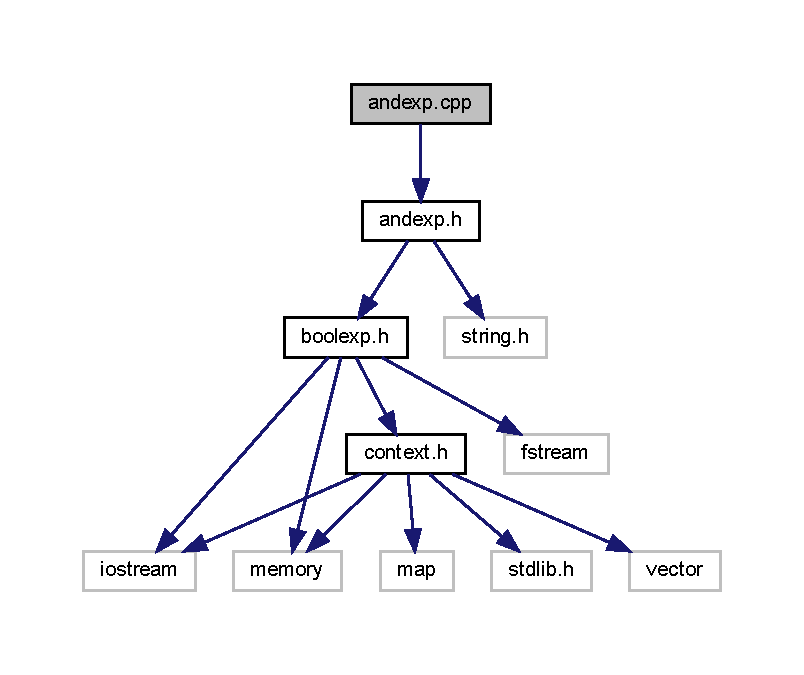
\includegraphics[width=350pt]{andexp_8cpp__incl}
\end{center}
\end{figure}

\hypertarget{andexp_8h}{}\section{andexp.\+h File Reference}
\label{andexp_8h}\index{andexp.\+h@{andexp.\+h}}
{\ttfamily \#include \char`\"{}boolexp.\+h\char`\"{}}\newline
{\ttfamily \#include $<$string.\+h$>$}\newline
Include dependency graph for andexp.\+h\+:
\nopagebreak
\begin{figure}[H]
\begin{center}
\leavevmode
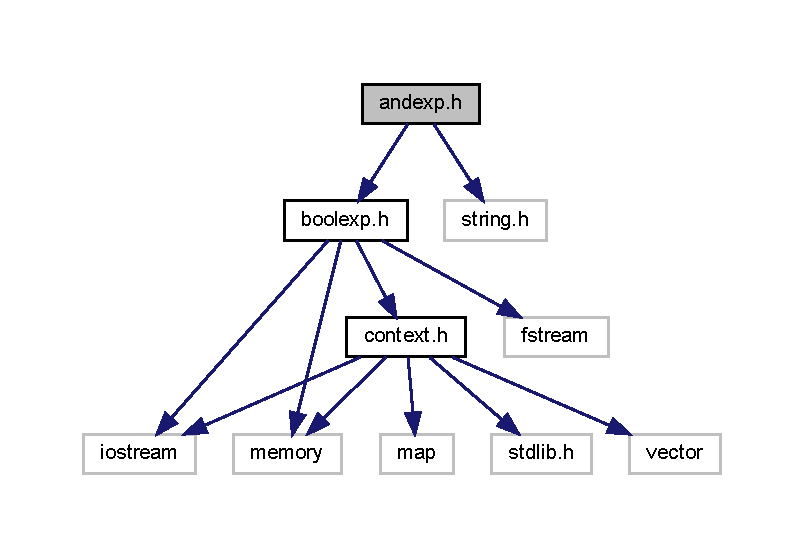
\includegraphics[width=350pt]{andexp_8h__incl}
\end{center}
\end{figure}
This graph shows which files directly or indirectly include this file\+:
\nopagebreak
\begin{figure}[H]
\begin{center}
\leavevmode
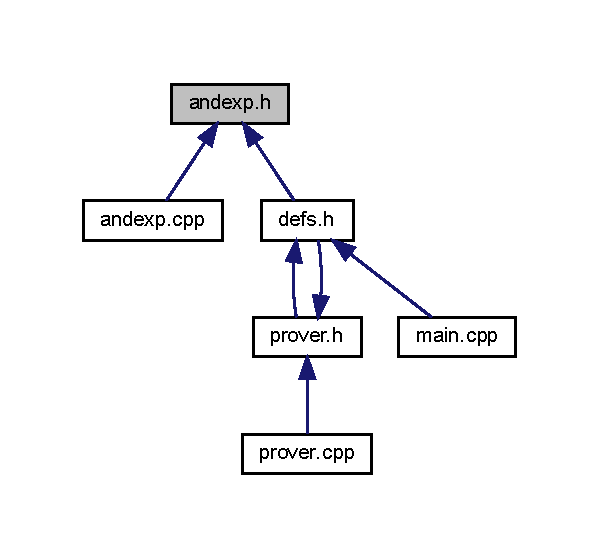
\includegraphics[width=288pt]{andexp_8h__dep__incl}
\end{center}
\end{figure}
\subsection*{Classes}
\begin{DoxyCompactItemize}
\item 
class \mbox{\hyperlink{classAndExp}{And\+Exp}}
\end{DoxyCompactItemize}

\hypertarget{boolexp_8cpp}{}\section{boolexp.\+cpp File Reference}
\label{boolexp_8cpp}\index{boolexp.\+cpp@{boolexp.\+cpp}}
{\ttfamily \#include \char`\"{}boolexp.\+h\char`\"{}}\newline
Include dependency graph for boolexp.\+cpp\+:
\nopagebreak
\begin{figure}[H]
\begin{center}
\leavevmode
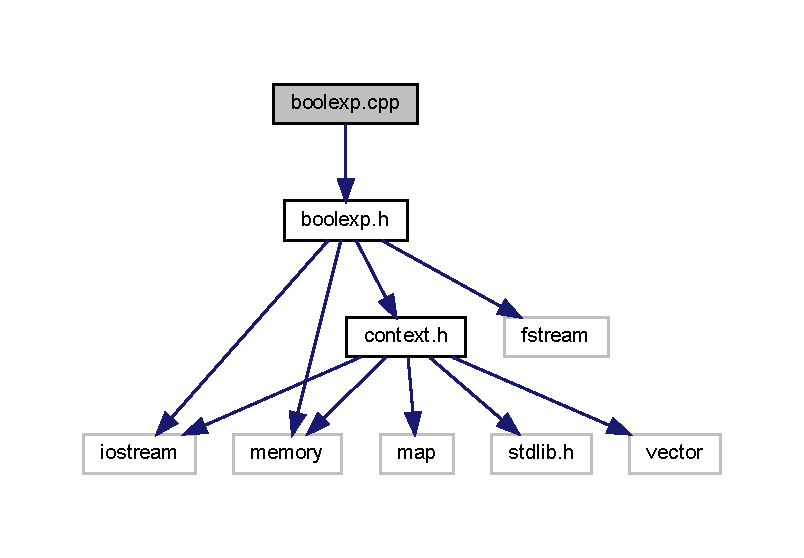
\includegraphics[width=350pt]{boolexp_8cpp__incl}
\end{center}
\end{figure}

\hypertarget{boolexp_8h}{}\section{boolexp.\+h File Reference}
\label{boolexp_8h}\index{boolexp.\+h@{boolexp.\+h}}
{\ttfamily \#include $<$iostream$>$}\newline
{\ttfamily \#include $<$fstream$>$}\newline
{\ttfamily \#include $<$memory$>$}\newline
{\ttfamily \#include \char`\"{}context.\+h\char`\"{}}\newline
Include dependency graph for boolexp.\+h\+:
\nopagebreak
\begin{figure}[H]
\begin{center}
\leavevmode
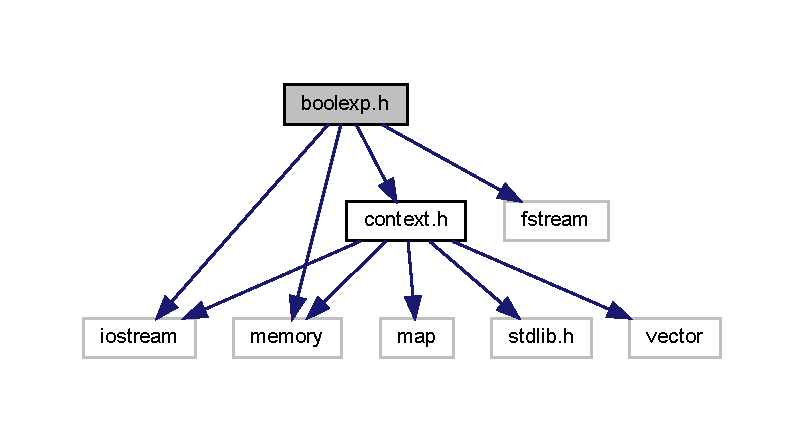
\includegraphics[width=350pt]{boolexp_8h__incl}
\end{center}
\end{figure}
This graph shows which files directly or indirectly include this file\+:
\nopagebreak
\begin{figure}[H]
\begin{center}
\leavevmode
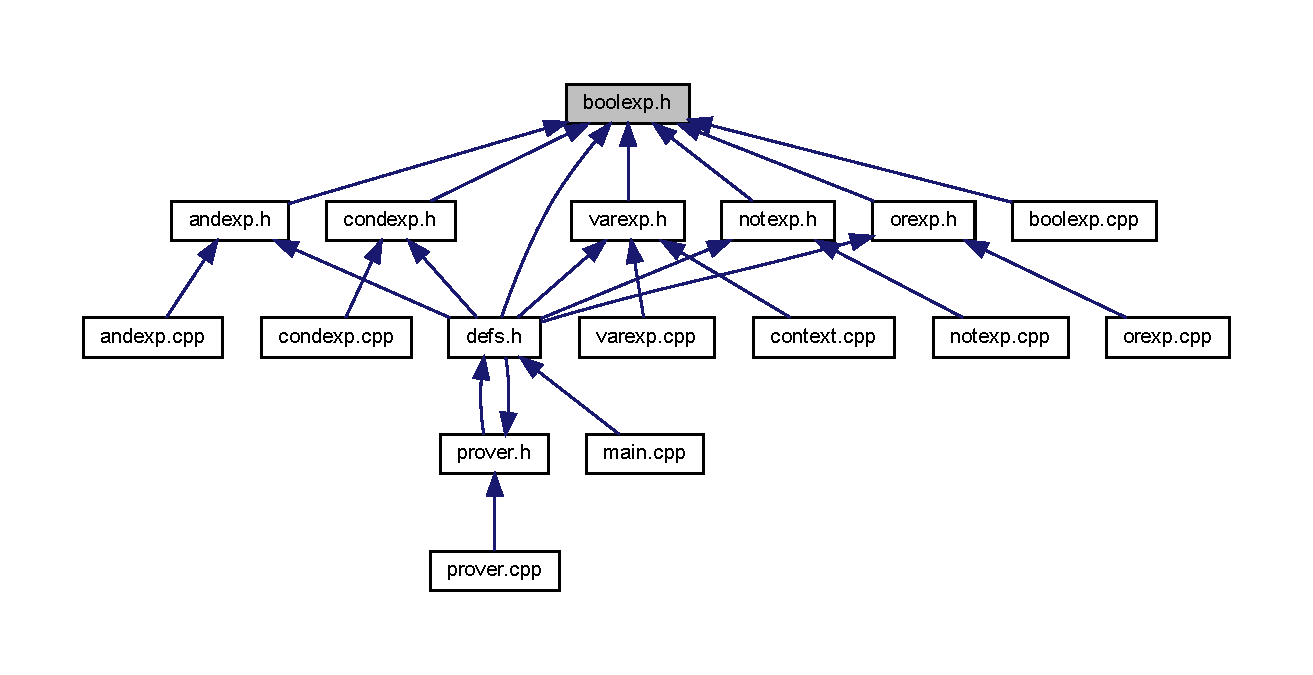
\includegraphics[width=350pt]{boolexp_8h__dep__incl}
\end{center}
\end{figure}
\subsection*{Classes}
\begin{DoxyCompactItemize}
\item 
struct \mbox{\hyperlink{structBoolReturn}{Bool\+Return}}
\item 
class \mbox{\hyperlink{classBoolExp}{Bool\+Exp}}
\end{DoxyCompactItemize}
\subsection*{Enumerations}
\begin{DoxyCompactItemize}
\item 
enum \mbox{\hyperlink{boolexp_8h_ac6a79184a0a7c1d2e3ea745512aa2d0c}{Prop\+Type}} \{ \newline
\mbox{\hyperlink{boolexp_8h_ac6a79184a0a7c1d2e3ea745512aa2d0ca04805a6faca1af084bc10a6966d6c028}{O\+R\+\_\+\+E\+XP}}, 
\mbox{\hyperlink{boolexp_8h_ac6a79184a0a7c1d2e3ea745512aa2d0ca2a7416697bd29ada986d099ced049f92}{V\+A\+R\+\_\+\+E\+XP}}, 
\mbox{\hyperlink{boolexp_8h_ac6a79184a0a7c1d2e3ea745512aa2d0ca085db57f00d8a4da06d4740433a8b554}{N\+O\+T\+\_\+\+E\+XP}}, 
\mbox{\hyperlink{boolexp_8h_ac6a79184a0a7c1d2e3ea745512aa2d0cab50e10e823f44f49914780f9e97e0805}{A\+N\+D\+\_\+\+E\+XP}}, 
\newline
\mbox{\hyperlink{boolexp_8h_ac6a79184a0a7c1d2e3ea745512aa2d0ca2bc6ba5f3e73884ee8865c9cb46522e7}{C\+O\+N\+D\+\_\+\+E\+XP}}
 \}
\end{DoxyCompactItemize}


\subsection{Enumeration Type Documentation}
\mbox{\Hypertarget{boolexp_8h_ac6a79184a0a7c1d2e3ea745512aa2d0c}\label{boolexp_8h_ac6a79184a0a7c1d2e3ea745512aa2d0c}} 
\index{boolexp.\+h@{boolexp.\+h}!Prop\+Type@{Prop\+Type}}
\index{Prop\+Type@{Prop\+Type}!boolexp.\+h@{boolexp.\+h}}
\subsubsection{\texorpdfstring{Prop\+Type}{PropType}}
{\footnotesize\ttfamily enum \mbox{\hyperlink{boolexp_8h_ac6a79184a0a7c1d2e3ea745512aa2d0c}{Prop\+Type}}}

Prop\+Type is used so that an expression can announce it\textquotesingle{}s own type and so that functions can do different things for differrent kinds of expressions \begin{DoxyEnumFields}{Enumerator}
\raisebox{\heightof{T}}[0pt][0pt]{\index{O\+R\+\_\+\+E\+XP@{O\+R\+\_\+\+E\+XP}!boolexp.\+h@{boolexp.\+h}}\index{boolexp.\+h@{boolexp.\+h}!O\+R\+\_\+\+E\+XP@{O\+R\+\_\+\+E\+XP}}}\mbox{\Hypertarget{boolexp_8h_ac6a79184a0a7c1d2e3ea745512aa2d0ca04805a6faca1af084bc10a6966d6c028}\label{boolexp_8h_ac6a79184a0a7c1d2e3ea745512aa2d0ca04805a6faca1af084bc10a6966d6c028}} 
O\+R\+\_\+\+E\+XP&The type for an OR expression \\
\hline

\raisebox{\heightof{T}}[0pt][0pt]{\index{V\+A\+R\+\_\+\+E\+XP@{V\+A\+R\+\_\+\+E\+XP}!boolexp.\+h@{boolexp.\+h}}\index{boolexp.\+h@{boolexp.\+h}!V\+A\+R\+\_\+\+E\+XP@{V\+A\+R\+\_\+\+E\+XP}}}\mbox{\Hypertarget{boolexp_8h_ac6a79184a0a7c1d2e3ea745512aa2d0ca2a7416697bd29ada986d099ced049f92}\label{boolexp_8h_ac6a79184a0a7c1d2e3ea745512aa2d0ca2a7416697bd29ada986d099ced049f92}} 
V\+A\+R\+\_\+\+E\+XP&The type for a Variable expression \\
\hline

\raisebox{\heightof{T}}[0pt][0pt]{\index{N\+O\+T\+\_\+\+E\+XP@{N\+O\+T\+\_\+\+E\+XP}!boolexp.\+h@{boolexp.\+h}}\index{boolexp.\+h@{boolexp.\+h}!N\+O\+T\+\_\+\+E\+XP@{N\+O\+T\+\_\+\+E\+XP}}}\mbox{\Hypertarget{boolexp_8h_ac6a79184a0a7c1d2e3ea745512aa2d0ca085db57f00d8a4da06d4740433a8b554}\label{boolexp_8h_ac6a79184a0a7c1d2e3ea745512aa2d0ca085db57f00d8a4da06d4740433a8b554}} 
N\+O\+T\+\_\+\+E\+XP&The type for a N\+OT expression \\
\hline

\raisebox{\heightof{T}}[0pt][0pt]{\index{A\+N\+D\+\_\+\+E\+XP@{A\+N\+D\+\_\+\+E\+XP}!boolexp.\+h@{boolexp.\+h}}\index{boolexp.\+h@{boolexp.\+h}!A\+N\+D\+\_\+\+E\+XP@{A\+N\+D\+\_\+\+E\+XP}}}\mbox{\Hypertarget{boolexp_8h_ac6a79184a0a7c1d2e3ea745512aa2d0cab50e10e823f44f49914780f9e97e0805}\label{boolexp_8h_ac6a79184a0a7c1d2e3ea745512aa2d0cab50e10e823f44f49914780f9e97e0805}} 
A\+N\+D\+\_\+\+E\+XP&The type for an A\+ND expression \\
\hline

\raisebox{\heightof{T}}[0pt][0pt]{\index{C\+O\+N\+D\+\_\+\+E\+XP@{C\+O\+N\+D\+\_\+\+E\+XP}!boolexp.\+h@{boolexp.\+h}}\index{boolexp.\+h@{boolexp.\+h}!C\+O\+N\+D\+\_\+\+E\+XP@{C\+O\+N\+D\+\_\+\+E\+XP}}}\mbox{\Hypertarget{boolexp_8h_ac6a79184a0a7c1d2e3ea745512aa2d0ca2bc6ba5f3e73884ee8865c9cb46522e7}\label{boolexp_8h_ac6a79184a0a7c1d2e3ea745512aa2d0ca2bc6ba5f3e73884ee8865c9cb46522e7}} 
C\+O\+N\+D\+\_\+\+E\+XP&The type for an Conditional expression \\
\hline

\end{DoxyEnumFields}

\hypertarget{calcTranslator_2translator_8cpp}{}\section{calc\+Translator/translator.cpp File Reference}
\label{calcTranslator_2translator_8cpp}\index{calc\+Translator/translator.\+cpp@{calc\+Translator/translator.\+cpp}}
{\ttfamily \#include $<$iostream$>$}\newline
{\ttfamily \#include $<$fstream$>$}\newline
{\ttfamily \#include $<$vector$>$}\newline
{\ttfamily \#include $<$string$>$}\newline
Include dependency graph for translator.\+cpp\+:
\nopagebreak
\begin{figure}[H]
\begin{center}
\leavevmode
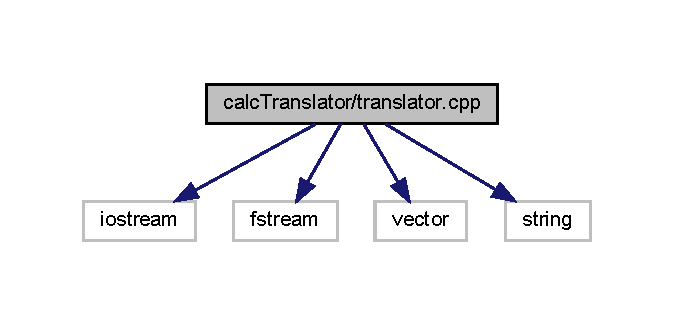
\includegraphics[width=324pt]{calcTranslator_2translator_8cpp__incl}
\end{center}
\end{figure}
\subsection*{Functions}
\begin{DoxyCompactItemize}
\item 
int \mbox{\hyperlink{calcTranslator_2translator_8cpp_a032a2170f1d2ae4cc1b1f71d49583501}{read\+Formula}} (istream \&, string \&)
\item 
int \mbox{\hyperlink{calcTranslator_2translator_8cpp_a9a98a53ceb07c3caa4b0bc9f04f4e81b}{parse\+Formula}} (ofstream \&, const string \&, int, int, vector$<$ string $>$ \&)
\item 
bool \mbox{\hyperlink{calcTranslator_2translator_8cpp_ab5f4eef1e3fc90a71b6241fcf4fb6024}{is\+Last\+Formula}} ()
\item 
int \mbox{\hyperlink{calcTranslator_2translator_8cpp_a79ea3585320c2302e9a2a3dd2155c809}{match\+End\+Parens}} (const string \&, int)
\item 
void \mbox{\hyperlink{calcTranslator_2translator_8cpp_afa0c885aab557e8d1acfc7a88f193685}{here\+Doc\+Preamble}} (ofstream \&)
\item 
void \mbox{\hyperlink{calcTranslator_2translator_8cpp_a332a39223773d14b8915f5f498c10891}{remove\+White\+Space}} (string \&)
\item 
int \mbox{\hyperlink{calcTranslator_2translator_8cpp_adf94c18dcb1bbdb492c07808af34bb6f}{is\+Variable}} (const string \&)
\item 
int \mbox{\hyperlink{calcTranslator_2translator_8cpp_a972ff985f6e91b57ec446f163780ea87}{is\+Conditional}} (const string \&)
\item 
int \mbox{\hyperlink{calcTranslator_2translator_8cpp_a7ddedf1549ca30c29da0ec84f483ccc5}{is\+And}} (const string \&)
\item 
int \mbox{\hyperlink{calcTranslator_2translator_8cpp_ac92f080c31a237e569ea813b14f61696}{is\+Or}} (const string \&)
\item 
int \mbox{\hyperlink{calcTranslator_2translator_8cpp_a32aef3652dc642a7f07782dcc4643802}{is\+Not}} (const string \&)
\item 
void \mbox{\hyperlink{calcTranslator_2translator_8cpp_a3f8083256d256f465c8fb0d64a223121}{twoplaceemit}} (ofstream \&, const string \&, int, int, const string \&, vector$<$ string $>$ \&)
\item 
void \mbox{\hyperlink{calcTranslator_2translator_8cpp_ad45f2fa3afd8ca317bad4c87672694bb}{oneplaceemit}} (ofstream \&, const string \&, int, int, const string \&, vector$<$ string $>$ \&)
\item 
void \mbox{\hyperlink{calcTranslator_2translator_8cpp_aee78876746f0432b79f7a97b30cefa50}{ask\+And\+Emitbool\+Values}} (ofstream \&fout, vector$<$ string $>$ vars)
\item 
int \mbox{\hyperlink{calcTranslator_2translator_8cpp_ae66f6b31b5ad750f1fe042a706a4e3d4}{main}} ()
\end{DoxyCompactItemize}


\subsection{Function Documentation}
\mbox{\Hypertarget{calcTranslator_2translator_8cpp_aee78876746f0432b79f7a97b30cefa50}\label{calcTranslator_2translator_8cpp_aee78876746f0432b79f7a97b30cefa50}} 
\index{calc\+Translator/translator.\+cpp@{calc\+Translator/translator.\+cpp}!ask\+And\+Emitbool\+Values@{ask\+And\+Emitbool\+Values}}
\index{ask\+And\+Emitbool\+Values@{ask\+And\+Emitbool\+Values}!calc\+Translator/translator.\+cpp@{calc\+Translator/translator.\+cpp}}
\subsubsection{\texorpdfstring{ask\+And\+Emitbool\+Values()}{askAndEmitboolValues()}}
{\footnotesize\ttfamily void ask\+And\+Emitbool\+Values (\begin{DoxyParamCaption}\item[{ofstream \&}]{fout,  }\item[{vector$<$ string $>$}]{vars }\end{DoxyParamCaption})}

Prompt the user to input a value for each variable in the proof 
\begin{DoxyParams}{Parameters}
{\em fout} & the file to write values to \\
\hline
{\em vars} & a vector of strings containing each variable to give a value to \\
\hline
\end{DoxyParams}
\mbox{\Hypertarget{calcTranslator_2translator_8cpp_afa0c885aab557e8d1acfc7a88f193685}\label{calcTranslator_2translator_8cpp_afa0c885aab557e8d1acfc7a88f193685}} 
\index{calc\+Translator/translator.\+cpp@{calc\+Translator/translator.\+cpp}!here\+Doc\+Preamble@{here\+Doc\+Preamble}}
\index{here\+Doc\+Preamble@{here\+Doc\+Preamble}!calc\+Translator/translator.\+cpp@{calc\+Translator/translator.\+cpp}}
\subsubsection{\texorpdfstring{here\+Doc\+Preamble()}{hereDocPreamble()}}
{\footnotesize\ttfamily void here\+Doc\+Preamble (\begin{DoxyParamCaption}\item[{ofstream \&}]{fout }\end{DoxyParamCaption})}

emit the heredoc preamble code to a file 
\begin{DoxyParams}{Parameters}
{\em fout} & the ofstream to output to \\
\hline
\end{DoxyParams}
\mbox{\Hypertarget{calcTranslator_2translator_8cpp_a7ddedf1549ca30c29da0ec84f483ccc5}\label{calcTranslator_2translator_8cpp_a7ddedf1549ca30c29da0ec84f483ccc5}} 
\index{calc\+Translator/translator.\+cpp@{calc\+Translator/translator.\+cpp}!is\+And@{is\+And}}
\index{is\+And@{is\+And}!calc\+Translator/translator.\+cpp@{calc\+Translator/translator.\+cpp}}
\subsubsection{\texorpdfstring{is\+And()}{isAnd()}}
{\footnotesize\ttfamily int is\+And (\begin{DoxyParamCaption}\item[{const string \&}]{str }\end{DoxyParamCaption})}

check if the given string is an and 
\begin{DoxyParams}{Parameters}
{\em str} & the string to be analyzed \\
\hline
\end{DoxyParams}
\begin{DoxyReturn}{Returns}
returns 1 if the input string is an and returns -\/1 if not 
\end{DoxyReturn}
\mbox{\Hypertarget{calcTranslator_2translator_8cpp_a972ff985f6e91b57ec446f163780ea87}\label{calcTranslator_2translator_8cpp_a972ff985f6e91b57ec446f163780ea87}} 
\index{calc\+Translator/translator.\+cpp@{calc\+Translator/translator.\+cpp}!is\+Conditional@{is\+Conditional}}
\index{is\+Conditional@{is\+Conditional}!calc\+Translator/translator.\+cpp@{calc\+Translator/translator.\+cpp}}
\subsubsection{\texorpdfstring{is\+Conditional()}{isConditional()}}
{\footnotesize\ttfamily int is\+Conditional (\begin{DoxyParamCaption}\item[{const string \&}]{str }\end{DoxyParamCaption})}

check if the given string is a conditional 
\begin{DoxyParams}{Parameters}
{\em str} & the string to be analyzed \\
\hline
\end{DoxyParams}
\begin{DoxyReturn}{Returns}
returns 1 if the input string is a conditional and -\/1 if not 
\end{DoxyReturn}
\mbox{\Hypertarget{calcTranslator_2translator_8cpp_ab5f4eef1e3fc90a71b6241fcf4fb6024}\label{calcTranslator_2translator_8cpp_ab5f4eef1e3fc90a71b6241fcf4fb6024}} 
\index{calc\+Translator/translator.\+cpp@{calc\+Translator/translator.\+cpp}!is\+Last\+Formula@{is\+Last\+Formula}}
\index{is\+Last\+Formula@{is\+Last\+Formula}!calc\+Translator/translator.\+cpp@{calc\+Translator/translator.\+cpp}}
\subsubsection{\texorpdfstring{is\+Last\+Formula()}{isLastFormula()}}
{\footnotesize\ttfamily bool is\+Last\+Formula (\begin{DoxyParamCaption}{ }\end{DoxyParamCaption})}

ask the user if the previously entered formula was the last \begin{DoxyReturn}{Returns}
true if the user choose so returns false if not 
\end{DoxyReturn}
\mbox{\Hypertarget{calcTranslator_2translator_8cpp_a32aef3652dc642a7f07782dcc4643802}\label{calcTranslator_2translator_8cpp_a32aef3652dc642a7f07782dcc4643802}} 
\index{calc\+Translator/translator.\+cpp@{calc\+Translator/translator.\+cpp}!is\+Not@{is\+Not}}
\index{is\+Not@{is\+Not}!calc\+Translator/translator.\+cpp@{calc\+Translator/translator.\+cpp}}
\subsubsection{\texorpdfstring{is\+Not()}{isNot()}}
{\footnotesize\ttfamily int is\+Not (\begin{DoxyParamCaption}\item[{const string \&}]{str }\end{DoxyParamCaption})}

check if the given string is a not 
\begin{DoxyParams}{Parameters}
{\em str} & the string to be analyzed \\
\hline
\end{DoxyParams}
\begin{DoxyReturn}{Returns}
returns 1 if the input string is a not and -\/1 if not 
\end{DoxyReturn}
\mbox{\Hypertarget{calcTranslator_2translator_8cpp_ac92f080c31a237e569ea813b14f61696}\label{calcTranslator_2translator_8cpp_ac92f080c31a237e569ea813b14f61696}} 
\index{calc\+Translator/translator.\+cpp@{calc\+Translator/translator.\+cpp}!is\+Or@{is\+Or}}
\index{is\+Or@{is\+Or}!calc\+Translator/translator.\+cpp@{calc\+Translator/translator.\+cpp}}
\subsubsection{\texorpdfstring{is\+Or()}{isOr()}}
{\footnotesize\ttfamily int is\+Or (\begin{DoxyParamCaption}\item[{const string \&}]{str }\end{DoxyParamCaption})}

check if the given string is an or 
\begin{DoxyParams}{Parameters}
{\em str} & the string to be analyzed \\
\hline
\end{DoxyParams}
\begin{DoxyReturn}{Returns}
returns 1 if the input string is an or returns -\/1 if not 
\end{DoxyReturn}
\mbox{\Hypertarget{calcTranslator_2translator_8cpp_adf94c18dcb1bbdb492c07808af34bb6f}\label{calcTranslator_2translator_8cpp_adf94c18dcb1bbdb492c07808af34bb6f}} 
\index{calc\+Translator/translator.\+cpp@{calc\+Translator/translator.\+cpp}!is\+Variable@{is\+Variable}}
\index{is\+Variable@{is\+Variable}!calc\+Translator/translator.\+cpp@{calc\+Translator/translator.\+cpp}}
\subsubsection{\texorpdfstring{is\+Variable()}{isVariable()}}
{\footnotesize\ttfamily int is\+Variable (\begin{DoxyParamCaption}\item[{const string \&}]{str }\end{DoxyParamCaption})}

check if the given string is a single propostional variable 
\begin{DoxyParams}{Parameters}
{\em str} & the string to be analyzed \\
\hline
\end{DoxyParams}
\begin{DoxyReturn}{Returns}
returns 1 if the input string is a variable and -\/1 if not 
\end{DoxyReturn}
\mbox{\Hypertarget{calcTranslator_2translator_8cpp_ae66f6b31b5ad750f1fe042a706a4e3d4}\label{calcTranslator_2translator_8cpp_ae66f6b31b5ad750f1fe042a706a4e3d4}} 
\index{calc\+Translator/translator.\+cpp@{calc\+Translator/translator.\+cpp}!main@{main}}
\index{main@{main}!calc\+Translator/translator.\+cpp@{calc\+Translator/translator.\+cpp}}
\subsubsection{\texorpdfstring{main()}{main()}}
{\footnotesize\ttfamily int main (\begin{DoxyParamCaption}{ }\end{DoxyParamCaption})}

\mbox{\Hypertarget{calcTranslator_2translator_8cpp_a79ea3585320c2302e9a2a3dd2155c809}\label{calcTranslator_2translator_8cpp_a79ea3585320c2302e9a2a3dd2155c809}} 
\index{calc\+Translator/translator.\+cpp@{calc\+Translator/translator.\+cpp}!match\+End\+Parens@{match\+End\+Parens}}
\index{match\+End\+Parens@{match\+End\+Parens}!calc\+Translator/translator.\+cpp@{calc\+Translator/translator.\+cpp}}
\subsubsection{\texorpdfstring{match\+End\+Parens()}{matchEndParens()}}
{\footnotesize\ttfamily int match\+End\+Parens (\begin{DoxyParamCaption}\item[{const string \&}]{str,  }\item[{int}]{start }\end{DoxyParamCaption})}

given a string and the index of an open paren return the index of it\textquotesingle{}s matching paren 
\begin{DoxyParams}{Parameters}
{\em str} & the string being analyzed \\
\hline
{\em start} & the opening paren to be matched \\
\hline
\end{DoxyParams}
\begin{DoxyReturn}{Returns}
returns the index of the required closing paren or -\/1 if it cannot find a closing paren 
\end{DoxyReturn}
\mbox{\Hypertarget{calcTranslator_2translator_8cpp_ad45f2fa3afd8ca317bad4c87672694bb}\label{calcTranslator_2translator_8cpp_ad45f2fa3afd8ca317bad4c87672694bb}} 
\index{calc\+Translator/translator.\+cpp@{calc\+Translator/translator.\+cpp}!oneplaceemit@{oneplaceemit}}
\index{oneplaceemit@{oneplaceemit}!calc\+Translator/translator.\+cpp@{calc\+Translator/translator.\+cpp}}
\subsubsection{\texorpdfstring{oneplaceemit()}{oneplaceemit()}}
{\footnotesize\ttfamily void oneplaceemit (\begin{DoxyParamCaption}\item[{ofstream \&}]{fout,  }\item[{const string \&}]{str,  }\item[{int}]{start,  }\item[{int}]{oploc,  }\item[{const string \&}]{op,  }\item[{vector$<$ string $>$ \&}]{vars }\end{DoxyParamCaption})}

emit the correct character sequence for a one character operator 
\begin{DoxyParams}{Parameters}
{\em fout} & the stream to output to \\
\hline
{\em str} & the string being analyzed \\
\hline
{\em start} & the starting point in the string to work on \\
\hline
{\em oploc} & the location of the operator in the expression \\
\hline
{\em op} & the operator that will be emitted \\
\hline
\end{DoxyParams}
\mbox{\Hypertarget{calcTranslator_2translator_8cpp_a9a98a53ceb07c3caa4b0bc9f04f4e81b}\label{calcTranslator_2translator_8cpp_a9a98a53ceb07c3caa4b0bc9f04f4e81b}} 
\index{calc\+Translator/translator.\+cpp@{calc\+Translator/translator.\+cpp}!parse\+Formula@{parse\+Formula}}
\index{parse\+Formula@{parse\+Formula}!calc\+Translator/translator.\+cpp@{calc\+Translator/translator.\+cpp}}
\subsubsection{\texorpdfstring{parse\+Formula()}{parseFormula()}}
{\footnotesize\ttfamily int parse\+Formula (\begin{DoxyParamCaption}\item[{ofstream \&}]{fout,  }\item[{const string \&}]{str,  }\item[{int}]{start,  }\item[{int}]{stop,  }\item[{vector$<$ string $>$ \&}]{vars }\end{DoxyParamCaption})}

recursively parse a formula and emit the correct sequence of characters to a file 
\begin{DoxyParams}{Parameters}
{\em fout} & the file stream to emit to \\
\hline
{\em the} & string to parse \\
\hline
{\em the} & start position in the string to parse from (possibly unnecessary) \\
\hline
{\em the} & ending position in the string to parse from (possibly unnecessary) \\
\hline
\end{DoxyParams}
\begin{DoxyReturn}{Returns}
currently returns 1 always but may return something more useful in the future 
\end{DoxyReturn}
\mbox{\Hypertarget{calcTranslator_2translator_8cpp_a032a2170f1d2ae4cc1b1f71d49583501}\label{calcTranslator_2translator_8cpp_a032a2170f1d2ae4cc1b1f71d49583501}} 
\index{calc\+Translator/translator.\+cpp@{calc\+Translator/translator.\+cpp}!read\+Formula@{read\+Formula}}
\index{read\+Formula@{read\+Formula}!calc\+Translator/translator.\+cpp@{calc\+Translator/translator.\+cpp}}
\subsubsection{\texorpdfstring{read\+Formula()}{readFormula()}}
{\footnotesize\ttfamily int read\+Formula (\begin{DoxyParamCaption}\item[{istream \&}]{instrm,  }\item[{string \&}]{str }\end{DoxyParamCaption})}

read a formula from the user into a string 
\begin{DoxyParams}{Parameters}
{\em the} & input stream to read from (probably not necessary) \\
\hline
{\em the} & string to read into \\
\hline
\end{DoxyParams}
\begin{DoxyReturn}{Returns}
currently returns 0 always but may return something more useful in the future 
\end{DoxyReturn}
\mbox{\Hypertarget{calcTranslator_2translator_8cpp_a332a39223773d14b8915f5f498c10891}\label{calcTranslator_2translator_8cpp_a332a39223773d14b8915f5f498c10891}} 
\index{calc\+Translator/translator.\+cpp@{calc\+Translator/translator.\+cpp}!remove\+White\+Space@{remove\+White\+Space}}
\index{remove\+White\+Space@{remove\+White\+Space}!calc\+Translator/translator.\+cpp@{calc\+Translator/translator.\+cpp}}
\subsubsection{\texorpdfstring{remove\+White\+Space()}{removeWhiteSpace()}}
{\footnotesize\ttfamily void remove\+White\+Space (\begin{DoxyParamCaption}\item[{string \&}]{str }\end{DoxyParamCaption})}

remove space characters from the input string 
\begin{DoxyParams}{Parameters}
{\em str} & the string having whitespace removed \\
\hline
\end{DoxyParams}
\mbox{\Hypertarget{calcTranslator_2translator_8cpp_a3f8083256d256f465c8fb0d64a223121}\label{calcTranslator_2translator_8cpp_a3f8083256d256f465c8fb0d64a223121}} 
\index{calc\+Translator/translator.\+cpp@{calc\+Translator/translator.\+cpp}!twoplaceemit@{twoplaceemit}}
\index{twoplaceemit@{twoplaceemit}!calc\+Translator/translator.\+cpp@{calc\+Translator/translator.\+cpp}}
\subsubsection{\texorpdfstring{twoplaceemit()}{twoplaceemit()}}
{\footnotesize\ttfamily void twoplaceemit (\begin{DoxyParamCaption}\item[{ofstream \&}]{fout,  }\item[{const string \&}]{str,  }\item[{int}]{start,  }\item[{int}]{oploc,  }\item[{const string \&}]{op,  }\item[{vector$<$ string $>$ \&}]{vars }\end{DoxyParamCaption})}

emit the correct character sequence for a two character operator 
\begin{DoxyParams}{Parameters}
{\em fout} & the stream to output to \\
\hline
{\em str} & the string being analyzed \\
\hline
{\em start} & the starting point in the string to work on \\
\hline
{\em oploc} & the location of the first character of the operator in the expression \\
\hline
{\em op} & the operator that will be emitted \\
\hline
\end{DoxyParams}

\hypertarget{proofTranslator_2translator_8cpp}{}\section{proof\+Translator/translator.cpp File Reference}
\label{proofTranslator_2translator_8cpp}\index{proof\+Translator/translator.\+cpp@{proof\+Translator/translator.\+cpp}}
{\ttfamily \#include $<$iostream$>$}\newline
{\ttfamily \#include $<$fstream$>$}\newline
Include dependency graph for translator.\+cpp\+:
\nopagebreak
\begin{figure}[H]
\begin{center}
\leavevmode
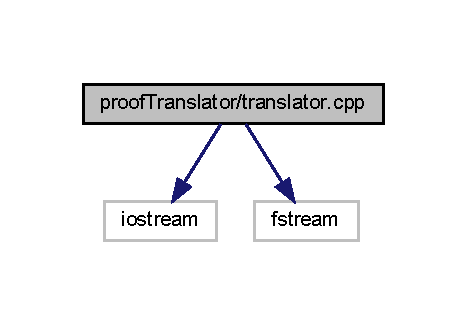
\includegraphics[width=224pt]{proofTranslator_2translator_8cpp__incl}
\end{center}
\end{figure}
\subsection*{Functions}
\begin{DoxyCompactItemize}
\item 
int \mbox{\hyperlink{proofTranslator_2translator_8cpp_a2f7913270ab9e4dbcc0bf9412ea26f0b}{read\+Formula}} (istream \&instrm, string \&str)
\item 
int \mbox{\hyperlink{proofTranslator_2translator_8cpp_a0604e7459787c8f3387008a1e5a41c24}{parse\+Formula}} (ofstream \&fout, const string \&str, int start, int stop)
\item 
bool \mbox{\hyperlink{proofTranslator_2translator_8cpp_ab5f4eef1e3fc90a71b6241fcf4fb6024}{is\+Last\+Formula}} ()
\item 
int \mbox{\hyperlink{proofTranslator_2translator_8cpp_aaf8fc732865f459a3cee6fa7d4c4375f}{match\+End\+Parens}} (const string \&str, int start)
\item 
void \mbox{\hyperlink{proofTranslator_2translator_8cpp_ad27b55e5788fde384fbc0edc063934e0}{here\+Doc\+Preamble}} (ofstream \&fout)
\item 
void \mbox{\hyperlink{proofTranslator_2translator_8cpp_a98ce518ad3ac0466f0e17edb45d25e62}{remove\+White\+Space}} (string \&str)
\item 
int \mbox{\hyperlink{proofTranslator_2translator_8cpp_af39eee8557efea6ff599ac6cc72c3b23}{is\+Variable}} (const string \&str)
\item 
int \mbox{\hyperlink{proofTranslator_2translator_8cpp_a972ff985f6e91b57ec446f163780ea87}{is\+Conditional}} (const string \&)
\item 
int \mbox{\hyperlink{proofTranslator_2translator_8cpp_a7ddedf1549ca30c29da0ec84f483ccc5}{is\+And}} (const string \&)
\item 
int \mbox{\hyperlink{proofTranslator_2translator_8cpp_ac92f080c31a237e569ea813b14f61696}{is\+Or}} (const string \&)
\item 
int \mbox{\hyperlink{proofTranslator_2translator_8cpp_a32aef3652dc642a7f07782dcc4643802}{is\+Not}} (const string \&)
\item 
void \mbox{\hyperlink{proofTranslator_2translator_8cpp_a889f06c5a06aeb9561d4eb653940a995}{twoplaceemit}} (ofstream \&fout, const string \&str, int start, int oploc, const string \&op)
\item 
void \mbox{\hyperlink{proofTranslator_2translator_8cpp_aa438b6e9ea8a924375884fa9eda28c2a}{oneplaceemit}} (ofstream \&fout, const string \&str, int start, int oploc, const string \&op)
\item 
int \mbox{\hyperlink{proofTranslator_2translator_8cpp_ae66f6b31b5ad750f1fe042a706a4e3d4}{main}} ()
\end{DoxyCompactItemize}


\subsection{Function Documentation}
\mbox{\Hypertarget{proofTranslator_2translator_8cpp_ad27b55e5788fde384fbc0edc063934e0}\label{proofTranslator_2translator_8cpp_ad27b55e5788fde384fbc0edc063934e0}} 
\index{proof\+Translator/translator.\+cpp@{proof\+Translator/translator.\+cpp}!here\+Doc\+Preamble@{here\+Doc\+Preamble}}
\index{here\+Doc\+Preamble@{here\+Doc\+Preamble}!proof\+Translator/translator.\+cpp@{proof\+Translator/translator.\+cpp}}
\subsubsection{\texorpdfstring{here\+Doc\+Preamble()}{hereDocPreamble()}}
{\footnotesize\ttfamily void here\+Doc\+Preamble (\begin{DoxyParamCaption}\item[{ofstream \&}]{fout }\end{DoxyParamCaption})}

emit the heredoc preamble code to a file 
\begin{DoxyParams}{Parameters}
{\em fout} & the ofstream to output to \\
\hline
\end{DoxyParams}
\mbox{\Hypertarget{proofTranslator_2translator_8cpp_a7ddedf1549ca30c29da0ec84f483ccc5}\label{proofTranslator_2translator_8cpp_a7ddedf1549ca30c29da0ec84f483ccc5}} 
\index{proof\+Translator/translator.\+cpp@{proof\+Translator/translator.\+cpp}!is\+And@{is\+And}}
\index{is\+And@{is\+And}!proof\+Translator/translator.\+cpp@{proof\+Translator/translator.\+cpp}}
\subsubsection{\texorpdfstring{is\+And()}{isAnd()}}
{\footnotesize\ttfamily int is\+And (\begin{DoxyParamCaption}\item[{const string \&}]{str }\end{DoxyParamCaption})}

check if the given string is an and 
\begin{DoxyParams}{Parameters}
{\em str} & the string to be analyzed \\
\hline
\end{DoxyParams}
\begin{DoxyReturn}{Returns}
returns 1 if the input string is an and returns -\/1 if not 
\end{DoxyReturn}
\mbox{\Hypertarget{proofTranslator_2translator_8cpp_a972ff985f6e91b57ec446f163780ea87}\label{proofTranslator_2translator_8cpp_a972ff985f6e91b57ec446f163780ea87}} 
\index{proof\+Translator/translator.\+cpp@{proof\+Translator/translator.\+cpp}!is\+Conditional@{is\+Conditional}}
\index{is\+Conditional@{is\+Conditional}!proof\+Translator/translator.\+cpp@{proof\+Translator/translator.\+cpp}}
\subsubsection{\texorpdfstring{is\+Conditional()}{isConditional()}}
{\footnotesize\ttfamily int is\+Conditional (\begin{DoxyParamCaption}\item[{const string \&}]{str }\end{DoxyParamCaption})}

check if the given string is a conditional 
\begin{DoxyParams}{Parameters}
{\em str} & the string to be analyzed \\
\hline
\end{DoxyParams}
\begin{DoxyReturn}{Returns}
returns 1 if the input string is a conditional and -\/1 if not 
\end{DoxyReturn}
\mbox{\Hypertarget{proofTranslator_2translator_8cpp_ab5f4eef1e3fc90a71b6241fcf4fb6024}\label{proofTranslator_2translator_8cpp_ab5f4eef1e3fc90a71b6241fcf4fb6024}} 
\index{proof\+Translator/translator.\+cpp@{proof\+Translator/translator.\+cpp}!is\+Last\+Formula@{is\+Last\+Formula}}
\index{is\+Last\+Formula@{is\+Last\+Formula}!proof\+Translator/translator.\+cpp@{proof\+Translator/translator.\+cpp}}
\subsubsection{\texorpdfstring{is\+Last\+Formula()}{isLastFormula()}}
{\footnotesize\ttfamily bool is\+Last\+Formula (\begin{DoxyParamCaption}{ }\end{DoxyParamCaption})}

ask the user if the previously entered formula was the last \begin{DoxyReturn}{Returns}
true if the user choose so returns false if not 
\end{DoxyReturn}
\mbox{\Hypertarget{proofTranslator_2translator_8cpp_a32aef3652dc642a7f07782dcc4643802}\label{proofTranslator_2translator_8cpp_a32aef3652dc642a7f07782dcc4643802}} 
\index{proof\+Translator/translator.\+cpp@{proof\+Translator/translator.\+cpp}!is\+Not@{is\+Not}}
\index{is\+Not@{is\+Not}!proof\+Translator/translator.\+cpp@{proof\+Translator/translator.\+cpp}}
\subsubsection{\texorpdfstring{is\+Not()}{isNot()}}
{\footnotesize\ttfamily int is\+Not (\begin{DoxyParamCaption}\item[{const string \&}]{str }\end{DoxyParamCaption})}

check if the given string is a not 
\begin{DoxyParams}{Parameters}
{\em str} & the string to be analyzed \\
\hline
\end{DoxyParams}
\begin{DoxyReturn}{Returns}
returns 1 if the input string is a not and -\/1 if not 
\end{DoxyReturn}
\mbox{\Hypertarget{proofTranslator_2translator_8cpp_ac92f080c31a237e569ea813b14f61696}\label{proofTranslator_2translator_8cpp_ac92f080c31a237e569ea813b14f61696}} 
\index{proof\+Translator/translator.\+cpp@{proof\+Translator/translator.\+cpp}!is\+Or@{is\+Or}}
\index{is\+Or@{is\+Or}!proof\+Translator/translator.\+cpp@{proof\+Translator/translator.\+cpp}}
\subsubsection{\texorpdfstring{is\+Or()}{isOr()}}
{\footnotesize\ttfamily int is\+Or (\begin{DoxyParamCaption}\item[{const string \&}]{str }\end{DoxyParamCaption})}

check if the given string is an or 
\begin{DoxyParams}{Parameters}
{\em str} & the string to be analyzed \\
\hline
\end{DoxyParams}
\begin{DoxyReturn}{Returns}
returns 1 if the input string is an or returns -\/1 if not 
\end{DoxyReturn}
\mbox{\Hypertarget{proofTranslator_2translator_8cpp_af39eee8557efea6ff599ac6cc72c3b23}\label{proofTranslator_2translator_8cpp_af39eee8557efea6ff599ac6cc72c3b23}} 
\index{proof\+Translator/translator.\+cpp@{proof\+Translator/translator.\+cpp}!is\+Variable@{is\+Variable}}
\index{is\+Variable@{is\+Variable}!proof\+Translator/translator.\+cpp@{proof\+Translator/translator.\+cpp}}
\subsubsection{\texorpdfstring{is\+Variable()}{isVariable()}}
{\footnotesize\ttfamily int is\+Variable (\begin{DoxyParamCaption}\item[{const string \&}]{str }\end{DoxyParamCaption})}

check if the given string is a single propostional variable 
\begin{DoxyParams}{Parameters}
{\em str} & the string to be analyzed \\
\hline
\end{DoxyParams}
\begin{DoxyReturn}{Returns}
returns 1 if the input string is a variable and -\/1 if not 
\end{DoxyReturn}
\mbox{\Hypertarget{proofTranslator_2translator_8cpp_ae66f6b31b5ad750f1fe042a706a4e3d4}\label{proofTranslator_2translator_8cpp_ae66f6b31b5ad750f1fe042a706a4e3d4}} 
\index{proof\+Translator/translator.\+cpp@{proof\+Translator/translator.\+cpp}!main@{main}}
\index{main@{main}!proof\+Translator/translator.\+cpp@{proof\+Translator/translator.\+cpp}}
\subsubsection{\texorpdfstring{main()}{main()}}
{\footnotesize\ttfamily int main (\begin{DoxyParamCaption}{ }\end{DoxyParamCaption})}

\mbox{\Hypertarget{proofTranslator_2translator_8cpp_aaf8fc732865f459a3cee6fa7d4c4375f}\label{proofTranslator_2translator_8cpp_aaf8fc732865f459a3cee6fa7d4c4375f}} 
\index{proof\+Translator/translator.\+cpp@{proof\+Translator/translator.\+cpp}!match\+End\+Parens@{match\+End\+Parens}}
\index{match\+End\+Parens@{match\+End\+Parens}!proof\+Translator/translator.\+cpp@{proof\+Translator/translator.\+cpp}}
\subsubsection{\texorpdfstring{match\+End\+Parens()}{matchEndParens()}}
{\footnotesize\ttfamily int match\+End\+Parens (\begin{DoxyParamCaption}\item[{const string \&}]{str,  }\item[{int}]{start }\end{DoxyParamCaption})}

given a string and the index of an open paren return the index of it\textquotesingle{}s matching paren 
\begin{DoxyParams}{Parameters}
{\em str} & the string being analyzed \\
\hline
{\em start} & the opening paren to be matched \\
\hline
\end{DoxyParams}
\begin{DoxyReturn}{Returns}
returns the index of the required closing paren or -\/1 if it cannot find a closing paren 
\end{DoxyReturn}
\mbox{\Hypertarget{proofTranslator_2translator_8cpp_aa438b6e9ea8a924375884fa9eda28c2a}\label{proofTranslator_2translator_8cpp_aa438b6e9ea8a924375884fa9eda28c2a}} 
\index{proof\+Translator/translator.\+cpp@{proof\+Translator/translator.\+cpp}!oneplaceemit@{oneplaceemit}}
\index{oneplaceemit@{oneplaceemit}!proof\+Translator/translator.\+cpp@{proof\+Translator/translator.\+cpp}}
\subsubsection{\texorpdfstring{oneplaceemit()}{oneplaceemit()}}
{\footnotesize\ttfamily void oneplaceemit (\begin{DoxyParamCaption}\item[{ofstream \&}]{fout,  }\item[{const string \&}]{str,  }\item[{int}]{start,  }\item[{int}]{oploc,  }\item[{const string \&}]{op }\end{DoxyParamCaption})}

emit the correct character sequence for a one character operator 
\begin{DoxyParams}{Parameters}
{\em fout} & the stream to output to \\
\hline
{\em str} & the string being analyzed \\
\hline
{\em start} & the starting point in the string to work on \\
\hline
{\em oploc} & the location of the operator in the expression \\
\hline
{\em op} & the operator that will be emitted \\
\hline
\end{DoxyParams}
\mbox{\Hypertarget{proofTranslator_2translator_8cpp_a0604e7459787c8f3387008a1e5a41c24}\label{proofTranslator_2translator_8cpp_a0604e7459787c8f3387008a1e5a41c24}} 
\index{proof\+Translator/translator.\+cpp@{proof\+Translator/translator.\+cpp}!parse\+Formula@{parse\+Formula}}
\index{parse\+Formula@{parse\+Formula}!proof\+Translator/translator.\+cpp@{proof\+Translator/translator.\+cpp}}
\subsubsection{\texorpdfstring{parse\+Formula()}{parseFormula()}}
{\footnotesize\ttfamily int parse\+Formula (\begin{DoxyParamCaption}\item[{ofstream \&}]{fout,  }\item[{const string \&}]{str,  }\item[{int}]{start,  }\item[{int}]{stop }\end{DoxyParamCaption})}

recursively parse a formula and emit the correct sequence of characters to a file 
\begin{DoxyParams}{Parameters}
{\em fout} & the file stream to emit to \\
\hline
{\em the} & string to parse \\
\hline
{\em the} & start position in the string to parse from (possibly unnecessary) \\
\hline
{\em the} & ending position in the string to parse from (possibly unnecessary) \\
\hline
\end{DoxyParams}
\begin{DoxyReturn}{Returns}
currently returns 1 always but may return something more useful in the future 
\end{DoxyReturn}
\mbox{\Hypertarget{proofTranslator_2translator_8cpp_a2f7913270ab9e4dbcc0bf9412ea26f0b}\label{proofTranslator_2translator_8cpp_a2f7913270ab9e4dbcc0bf9412ea26f0b}} 
\index{proof\+Translator/translator.\+cpp@{proof\+Translator/translator.\+cpp}!read\+Formula@{read\+Formula}}
\index{read\+Formula@{read\+Formula}!proof\+Translator/translator.\+cpp@{proof\+Translator/translator.\+cpp}}
\subsubsection{\texorpdfstring{read\+Formula()}{readFormula()}}
{\footnotesize\ttfamily int read\+Formula (\begin{DoxyParamCaption}\item[{istream \&}]{instrm,  }\item[{string \&}]{str }\end{DoxyParamCaption})}

read a formula from the user into a string 
\begin{DoxyParams}{Parameters}
{\em the} & input stream to read from (probably not necessary) \\
\hline
{\em the} & string to read into \\
\hline
\end{DoxyParams}
\begin{DoxyReturn}{Returns}
currently returns 0 always but may return something more useful in the future 
\end{DoxyReturn}
\mbox{\Hypertarget{proofTranslator_2translator_8cpp_a98ce518ad3ac0466f0e17edb45d25e62}\label{proofTranslator_2translator_8cpp_a98ce518ad3ac0466f0e17edb45d25e62}} 
\index{proof\+Translator/translator.\+cpp@{proof\+Translator/translator.\+cpp}!remove\+White\+Space@{remove\+White\+Space}}
\index{remove\+White\+Space@{remove\+White\+Space}!proof\+Translator/translator.\+cpp@{proof\+Translator/translator.\+cpp}}
\subsubsection{\texorpdfstring{remove\+White\+Space()}{removeWhiteSpace()}}
{\footnotesize\ttfamily void remove\+White\+Space (\begin{DoxyParamCaption}\item[{string \&}]{str }\end{DoxyParamCaption})}

remove space characters from the input string 
\begin{DoxyParams}{Parameters}
{\em str} & the string having whitespace removed \\
\hline
\end{DoxyParams}
\mbox{\Hypertarget{proofTranslator_2translator_8cpp_a889f06c5a06aeb9561d4eb653940a995}\label{proofTranslator_2translator_8cpp_a889f06c5a06aeb9561d4eb653940a995}} 
\index{proof\+Translator/translator.\+cpp@{proof\+Translator/translator.\+cpp}!twoplaceemit@{twoplaceemit}}
\index{twoplaceemit@{twoplaceemit}!proof\+Translator/translator.\+cpp@{proof\+Translator/translator.\+cpp}}
\subsubsection{\texorpdfstring{twoplaceemit()}{twoplaceemit()}}
{\footnotesize\ttfamily void twoplaceemit (\begin{DoxyParamCaption}\item[{ofstream \&}]{fout,  }\item[{const string \&}]{str,  }\item[{int}]{start,  }\item[{int}]{oploc,  }\item[{const string \&}]{op }\end{DoxyParamCaption})}

emit the correct character sequence for a two character operator 
\begin{DoxyParams}{Parameters}
{\em fout} & the stream to output to \\
\hline
{\em str} & the string being analyzed \\
\hline
{\em start} & the starting point in the string to work on \\
\hline
{\em oploc} & the location of the first character of the operator in the expression \\
\hline
{\em op} & the operator that will be emitted \\
\hline
\end{DoxyParams}

\hypertarget{condexp_8cpp}{}\section{condexp.\+cpp File Reference}
\label{condexp_8cpp}\index{condexp.\+cpp@{condexp.\+cpp}}
{\ttfamily \#include \char`\"{}condexp.\+h\char`\"{}}\newline
Include dependency graph for condexp.\+cpp\+:
\nopagebreak
\begin{figure}[H]
\begin{center}
\leavevmode
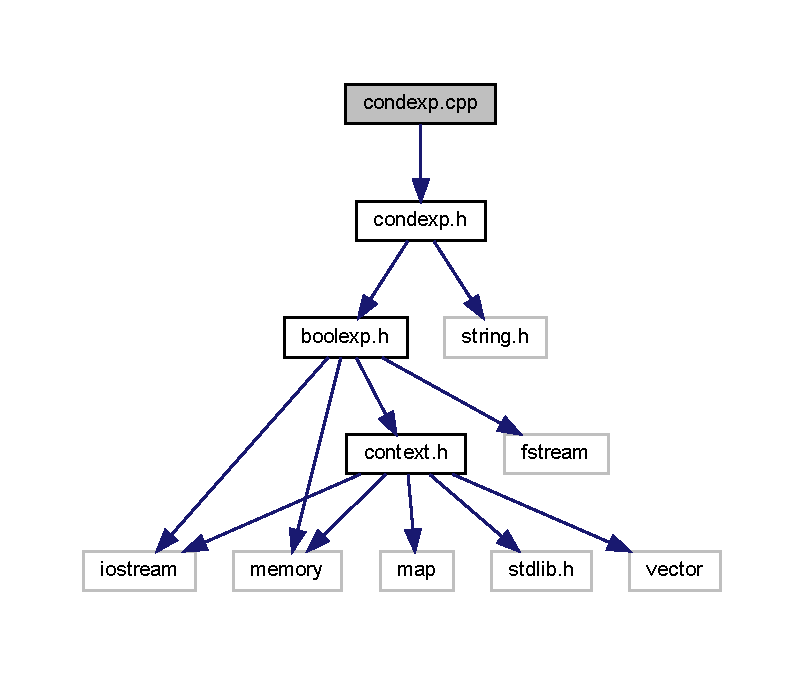
\includegraphics[width=350pt]{condexp_8cpp__incl}
\end{center}
\end{figure}

\hypertarget{condexp_8h}{}\section{condexp.\+h File Reference}
\label{condexp_8h}\index{condexp.\+h@{condexp.\+h}}
{\ttfamily \#include \char`\"{}boolexp.\+h\char`\"{}}\newline
{\ttfamily \#include $<$string.\+h$>$}\newline
Include dependency graph for condexp.\+h\+:
\nopagebreak
\begin{figure}[H]
\begin{center}
\leavevmode
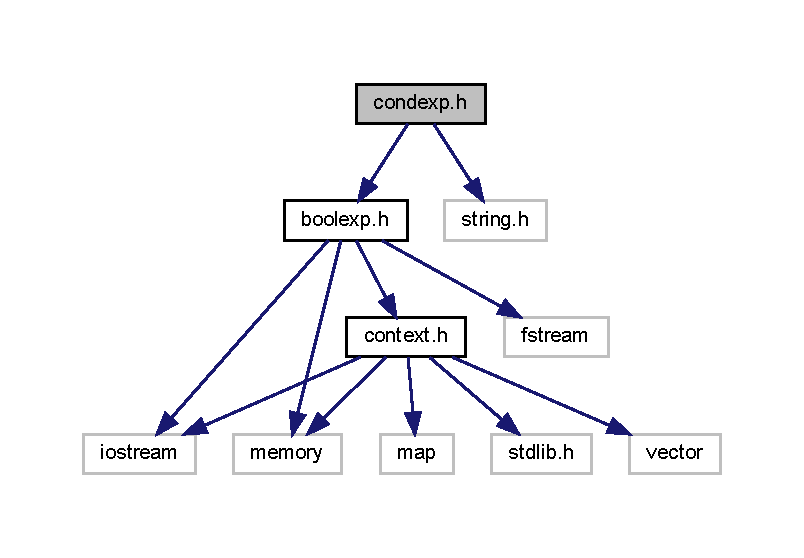
\includegraphics[width=350pt]{condexp_8h__incl}
\end{center}
\end{figure}
This graph shows which files directly or indirectly include this file\+:
\nopagebreak
\begin{figure}[H]
\begin{center}
\leavevmode
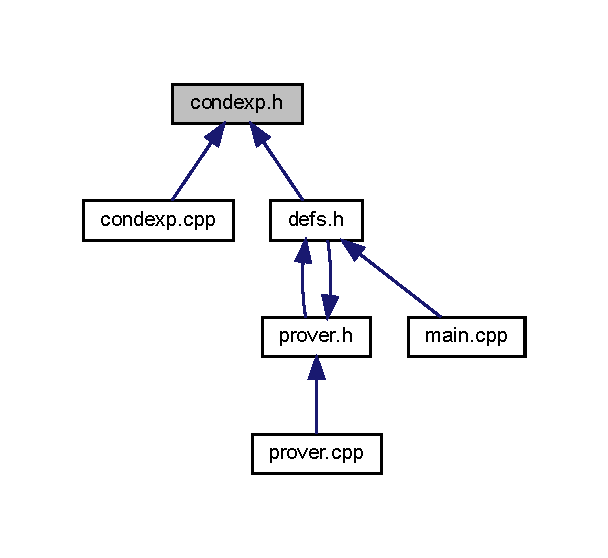
\includegraphics[width=292pt]{condexp_8h__dep__incl}
\end{center}
\end{figure}
\subsection*{Classes}
\begin{DoxyCompactItemize}
\item 
class \mbox{\hyperlink{classCondExp}{Cond\+Exp}}
\end{DoxyCompactItemize}

\hypertarget{context_8cpp}{}\section{context.\+cpp File Reference}
\label{context_8cpp}\index{context.\+cpp@{context.\+cpp}}
{\ttfamily \#include \char`\"{}context.\+h\char`\"{}}\newline
{\ttfamily \#include \char`\"{}varexp.\+h\char`\"{}}\newline
Include dependency graph for context.\+cpp\+:
\nopagebreak
\begin{figure}[H]
\begin{center}
\leavevmode
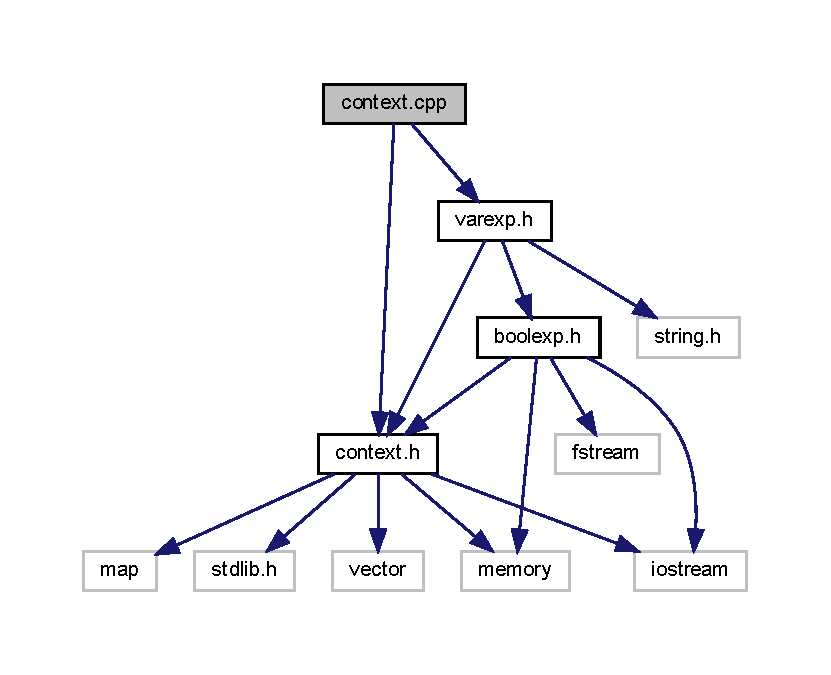
\includegraphics[width=350pt]{context_8cpp__incl}
\end{center}
\end{figure}

\hypertarget{context_8h}{}\section{context.\+h File Reference}
\label{context_8h}\index{context.\+h@{context.\+h}}
{\ttfamily \#include $<$iostream$>$}\newline
{\ttfamily \#include $<$map$>$}\newline
{\ttfamily \#include $<$stdlib.\+h$>$}\newline
{\ttfamily \#include $<$vector$>$}\newline
{\ttfamily \#include $<$memory$>$}\newline
Include dependency graph for context.\+h\+:
\nopagebreak
\begin{figure}[H]
\begin{center}
\leavevmode
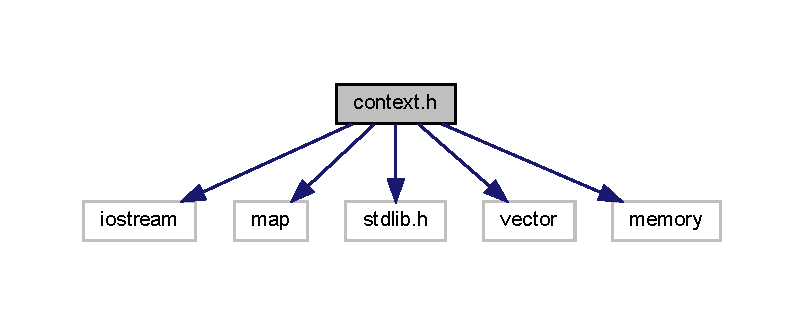
\includegraphics[width=350pt]{context_8h__incl}
\end{center}
\end{figure}
This graph shows which files directly or indirectly include this file\+:
\nopagebreak
\begin{figure}[H]
\begin{center}
\leavevmode
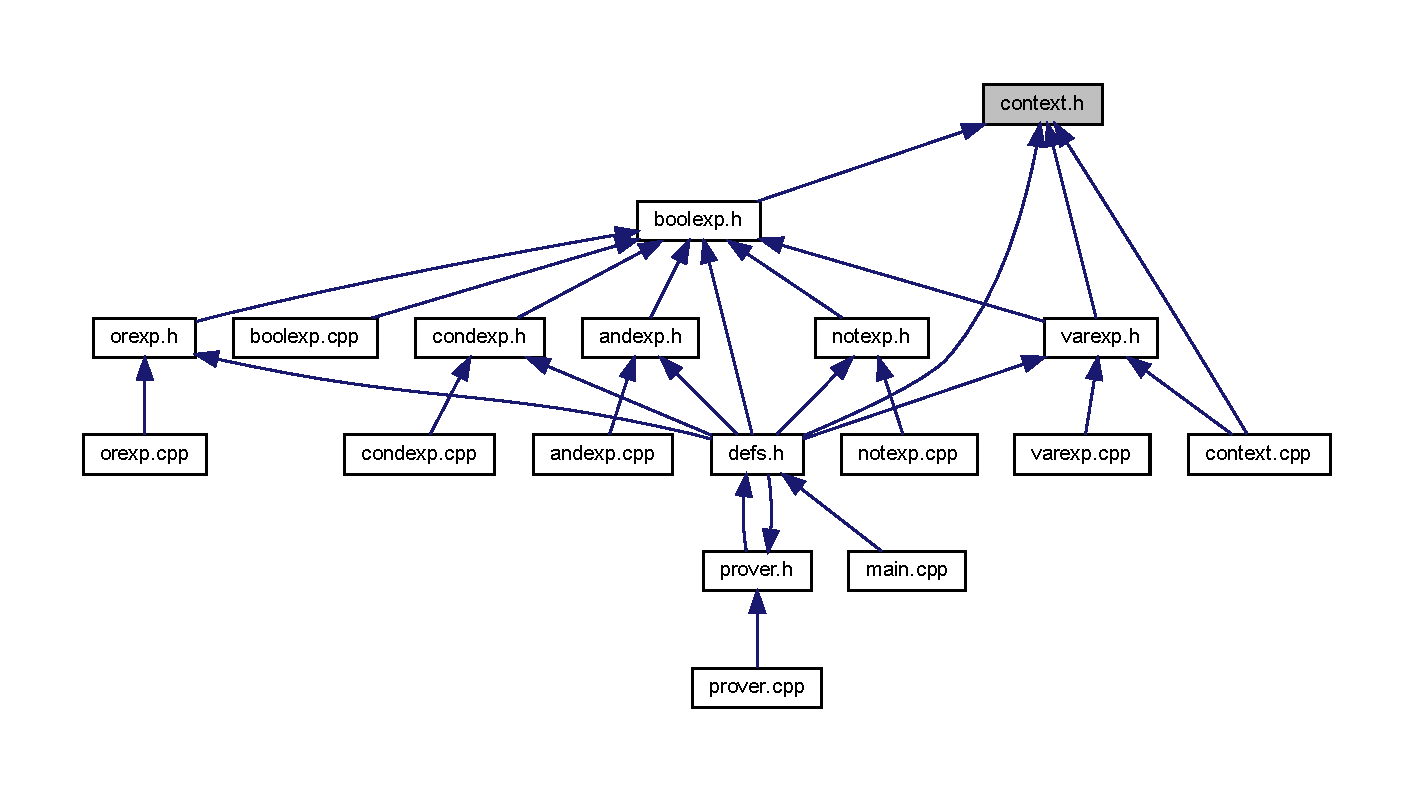
\includegraphics[width=350pt]{context_8h__dep__incl}
\end{center}
\end{figure}
\subsection*{Classes}
\begin{DoxyCompactItemize}
\item 
class \mbox{\hyperlink{classContext}{Context}}
\end{DoxyCompactItemize}

\hypertarget{defs_8h}{}\section{defs.\+h File Reference}
\label{defs_8h}\index{defs.\+h@{defs.\+h}}
{\ttfamily \#include \char`\"{}boolexp.\+h\char`\"{}}\newline
{\ttfamily \#include \char`\"{}context.\+h\char`\"{}}\newline
{\ttfamily \#include \char`\"{}varexp.\+h\char`\"{}}\newline
{\ttfamily \#include \char`\"{}notexp.\+h\char`\"{}}\newline
{\ttfamily \#include \char`\"{}andexp.\+h\char`\"{}}\newline
{\ttfamily \#include \char`\"{}orexp.\+h\char`\"{}}\newline
{\ttfamily \#include \char`\"{}condexp.\+h\char`\"{}}\newline
{\ttfamily \#include \char`\"{}prover.\+h\char`\"{}}\newline
Include dependency graph for defs.\+h\+:
\nopagebreak
\begin{figure}[H]
\begin{center}
\leavevmode
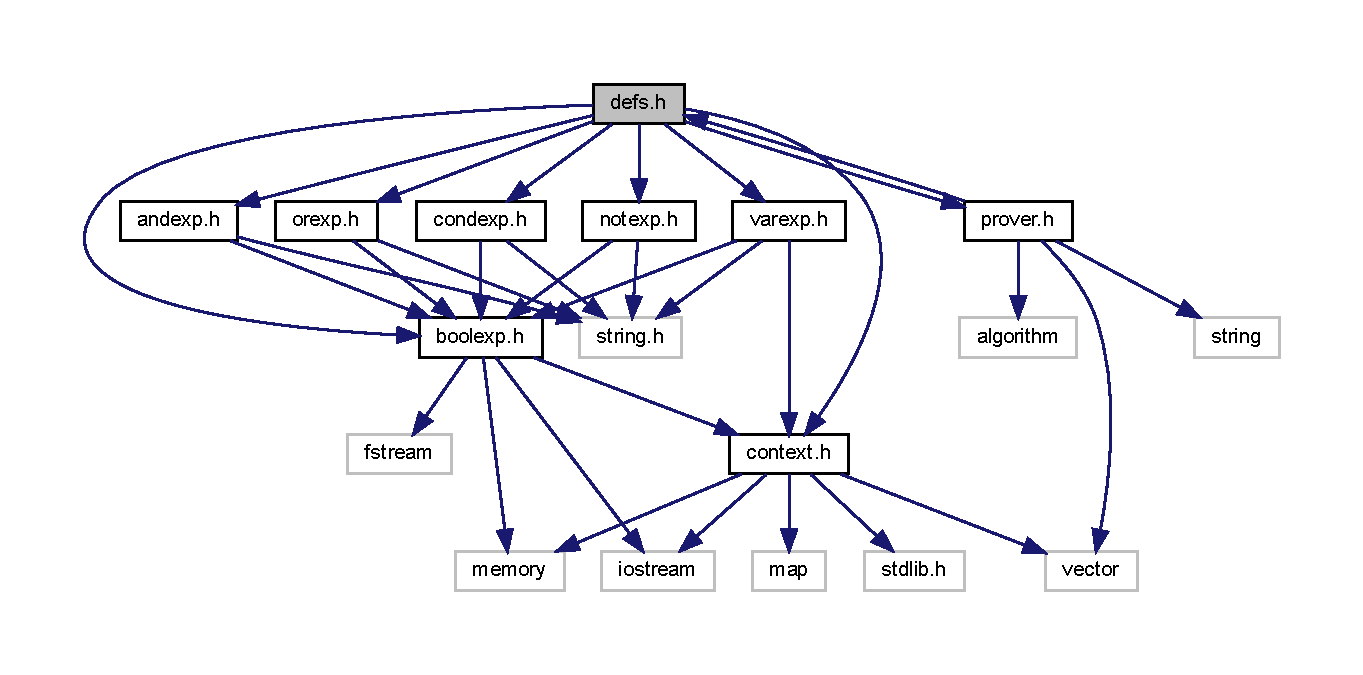
\includegraphics[width=350pt]{defs_8h__incl}
\end{center}
\end{figure}
This graph shows which files directly or indirectly include this file\+:
\nopagebreak
\begin{figure}[H]
\begin{center}
\leavevmode
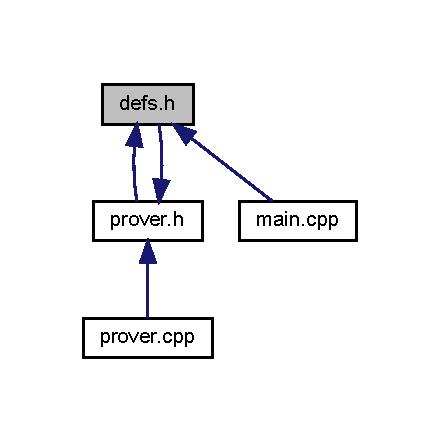
\includegraphics[width=211pt]{defs_8h__dep__incl}
\end{center}
\end{figure}

\hypertarget{examplecalculationwithtranslator_8dox}{}\section{doxfiles/examplecalculationwithtranslator.dox File Reference}
\label{examplecalculationwithtranslator_8dox}\index{doxfiles/examplecalculationwithtranslator.\+dox@{doxfiles/examplecalculationwithtranslator.\+dox}}

\hypertarget{exampleproofwithtranslator_8dox}{}\section{doxfiles/exampleproofwithtranslator.dox File Reference}
\label{exampleproofwithtranslator_8dox}\index{doxfiles/exampleproofwithtranslator.\+dox@{doxfiles/exampleproofwithtranslator.\+dox}}

\hypertarget{heredoc_8dox}{}\section{doxfiles/heredoc.dox File Reference}
\label{heredoc_8dox}\index{doxfiles/heredoc.\+dox@{doxfiles/heredoc.\+dox}}

\hypertarget{mainpage_8dox}{}\section{doxfiles/mainpage.dox File Reference}
\label{mainpage_8dox}\index{doxfiles/mainpage.\+dox@{doxfiles/mainpage.\+dox}}

\hypertarget{main_8cpp}{}\section{main.\+cpp File Reference}
\label{main_8cpp}\index{main.\+cpp@{main.\+cpp}}
{\ttfamily \#include \char`\"{}defs.\+h\char`\"{}}\newline
{\ttfamily \#include $<$math.\+h$>$}\newline
{\ttfamily \#include $<$algorithm$>$}\newline
Include dependency graph for main.\+cpp\+:
\nopagebreak
\begin{figure}[H]
\begin{center}
\leavevmode
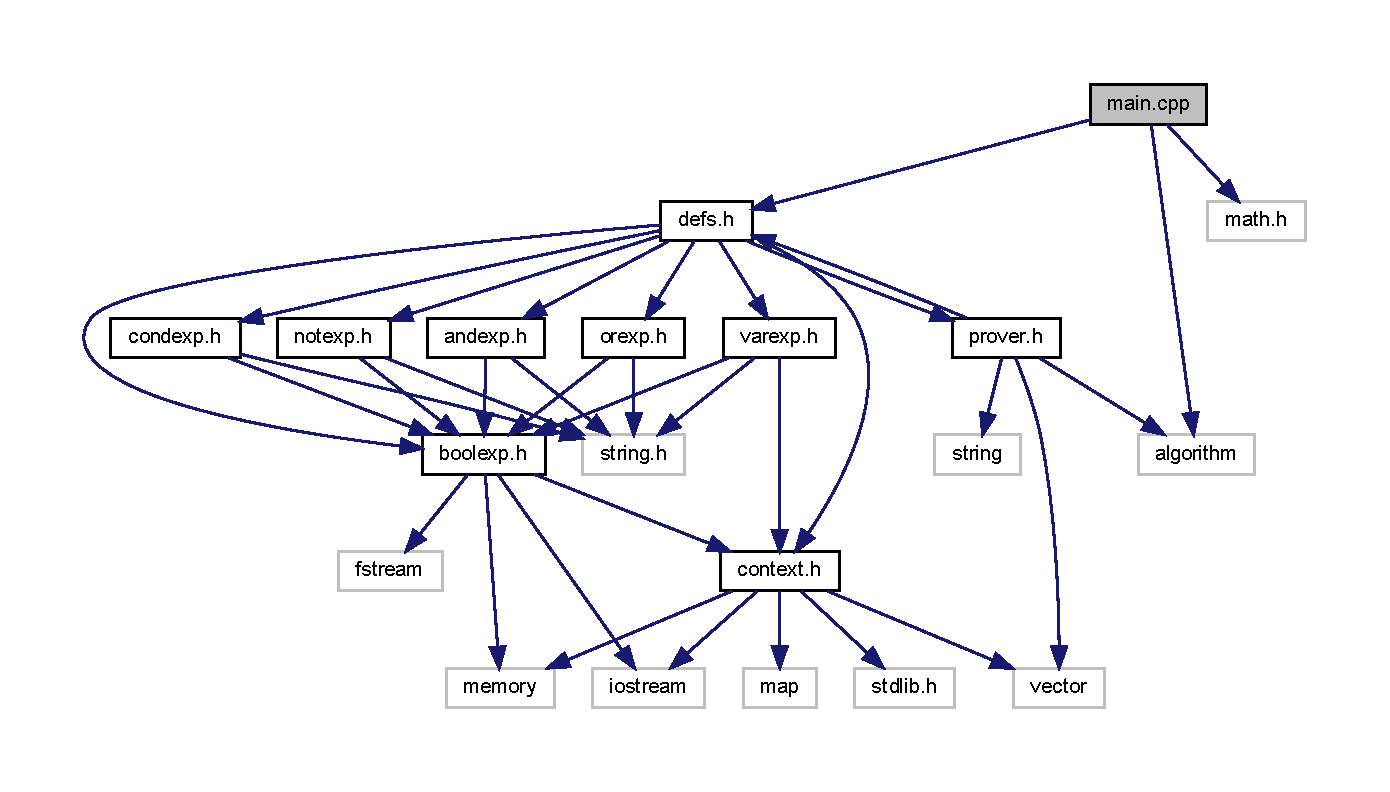
\includegraphics[width=350pt]{main_8cpp__incl}
\end{center}
\end{figure}
\subsection*{Functions}
\begin{DoxyCompactItemize}
\item 
shared\+\_\+ptr$<$ \mbox{\hyperlink{classBoolExp}{Bool\+Exp}} $>$ \mbox{\hyperlink{main_8cpp_a9e3ff65f2fed31d896a953c2218cb76a}{build\+Expr}} (shared\+\_\+ptr$<$ \mbox{\hyperlink{classBoolExp}{Bool\+Exp}} $>$ current, \mbox{\hyperlink{classContext}{Context}} \&context)
\item 
bool \mbox{\hyperlink{main_8cpp_abf28ae9d280d792ce0e4ffc084ff558d}{test\+Every\+Permutation}} (vector$<$ bool $>$ \&myvec, \mbox{\hyperlink{classProver}{Prover}} \&proof, \mbox{\hyperlink{classContext}{Context}} \&context, int premises, int conclusion)
\item 
int \mbox{\hyperlink{main_8cpp_aa4a2904d7f9dd719bb9f6ae3721560b1}{prover}} ()
\item 
int \mbox{\hyperlink{main_8cpp_a1d4f2ecda872542e9a237fb7fc32787c}{calculator}} ()
\item 
int \mbox{\hyperlink{main_8cpp_ae66f6b31b5ad750f1fe042a706a4e3d4}{main}} ()
\end{DoxyCompactItemize}


\subsection{Function Documentation}
\mbox{\Hypertarget{main_8cpp_a9e3ff65f2fed31d896a953c2218cb76a}\label{main_8cpp_a9e3ff65f2fed31d896a953c2218cb76a}} 
\index{main.\+cpp@{main.\+cpp}!build\+Expr@{build\+Expr}}
\index{build\+Expr@{build\+Expr}!main.\+cpp@{main.\+cpp}}
\subsubsection{\texorpdfstring{build\+Expr()}{buildExpr()}}
{\footnotesize\ttfamily shared\+\_\+ptr$<$ \mbox{\hyperlink{classBoolExp}{Bool\+Exp}} $>$ build\+Expr (\begin{DoxyParamCaption}\item[{shared\+\_\+ptr$<$ \mbox{\hyperlink{classBoolExp}{Bool\+Exp}} $>$}]{current,  }\item[{\mbox{\hyperlink{classContext}{Context}} \&}]{context }\end{DoxyParamCaption})}

builds a well formed formula based on user input via an interactive menu 
\begin{DoxyParams}{Parameters}
{\em current} & the current \mbox{\hyperlink{classBoolExp}{Bool\+Exp}} being created \\
\hline
{\em the} & context mapping variables to values \\
\hline
\end{DoxyParams}
\begin{DoxyReturn}{Returns}
returns a shared\+\_\+ptr$<$\+Bool\+Exp$>$ referring to the created formula 
\end{DoxyReturn}
\mbox{\Hypertarget{main_8cpp_a1d4f2ecda872542e9a237fb7fc32787c}\label{main_8cpp_a1d4f2ecda872542e9a237fb7fc32787c}} 
\index{main.\+cpp@{main.\+cpp}!calculator@{calculator}}
\index{calculator@{calculator}!main.\+cpp@{main.\+cpp}}
\subsubsection{\texorpdfstring{calculator()}{calculator()}}
{\footnotesize\ttfamily int calculator (\begin{DoxyParamCaption}{ }\end{DoxyParamCaption})}

the program is running in calculator mode the user will input formulas and values to be calculated \begin{DoxyReturn}{Returns}
indiscriminately returns 0 but may return something more useful in the future 
\end{DoxyReturn}
\mbox{\Hypertarget{main_8cpp_ae66f6b31b5ad750f1fe042a706a4e3d4}\label{main_8cpp_ae66f6b31b5ad750f1fe042a706a4e3d4}} 
\index{main.\+cpp@{main.\+cpp}!main@{main}}
\index{main@{main}!main.\+cpp@{main.\+cpp}}
\subsubsection{\texorpdfstring{main()}{main()}}
{\footnotesize\ttfamily int main (\begin{DoxyParamCaption}{ }\end{DoxyParamCaption})}

initiates either calculator or prover mode based on user input \mbox{\Hypertarget{main_8cpp_aa4a2904d7f9dd719bb9f6ae3721560b1}\label{main_8cpp_aa4a2904d7f9dd719bb9f6ae3721560b1}} 
\index{main.\+cpp@{main.\+cpp}!prover@{prover}}
\index{prover@{prover}!main.\+cpp@{main.\+cpp}}
\subsubsection{\texorpdfstring{prover()}{prover()}}
{\footnotesize\ttfamily int prover (\begin{DoxyParamCaption}{ }\end{DoxyParamCaption})}

the program is running in proof mode the user will input arguments to be proved or disproved \begin{DoxyReturn}{Returns}
indiscriminately returns 0 but may return something more useful in the future 
\end{DoxyReturn}
\mbox{\Hypertarget{main_8cpp_abf28ae9d280d792ce0e4ffc084ff558d}\label{main_8cpp_abf28ae9d280d792ce0e4ffc084ff558d}} 
\index{main.\+cpp@{main.\+cpp}!test\+Every\+Permutation@{test\+Every\+Permutation}}
\index{test\+Every\+Permutation@{test\+Every\+Permutation}!main.\+cpp@{main.\+cpp}}
\subsubsection{\texorpdfstring{test\+Every\+Permutation()}{testEveryPermutation()}}
{\footnotesize\ttfamily bool test\+Every\+Permutation (\begin{DoxyParamCaption}\item[{vector$<$ bool $>$ \&}]{myvec,  }\item[{\mbox{\hyperlink{classProver}{Prover}} \&}]{proof,  }\item[{\mbox{\hyperlink{classContext}{Context}} \&}]{context,  }\item[{int}]{premises,  }\item[{int}]{conclusion }\end{DoxyParamCaption})}

attempt to bruteforce a counterargument by testing every possible permutation 
\begin{DoxyParams}{Parameters}
{\em myvec} & a vector of bools containing one element for every formula \\
\hline
{\em proof} & the proof \\
\hline
{\em context} & the \mbox{\hyperlink{classContext}{Context}} structure mapping values to variables for this proof \\
\hline
{\em premises} & the count of premises \\
\hline
{\em conclusions} & the index of the conclusion in the proof \\
\hline
\end{DoxyParams}
\begin{DoxyReturn}{Returns}
returns true if a counterarg is found otherwise false 
\end{DoxyReturn}

\hypertarget{notexp_8cpp}{}\section{notexp.\+cpp File Reference}
\label{notexp_8cpp}\index{notexp.\+cpp@{notexp.\+cpp}}
{\ttfamily \#include \char`\"{}notexp.\+h\char`\"{}}\newline
Include dependency graph for notexp.\+cpp\+:
\nopagebreak
\begin{figure}[H]
\begin{center}
\leavevmode
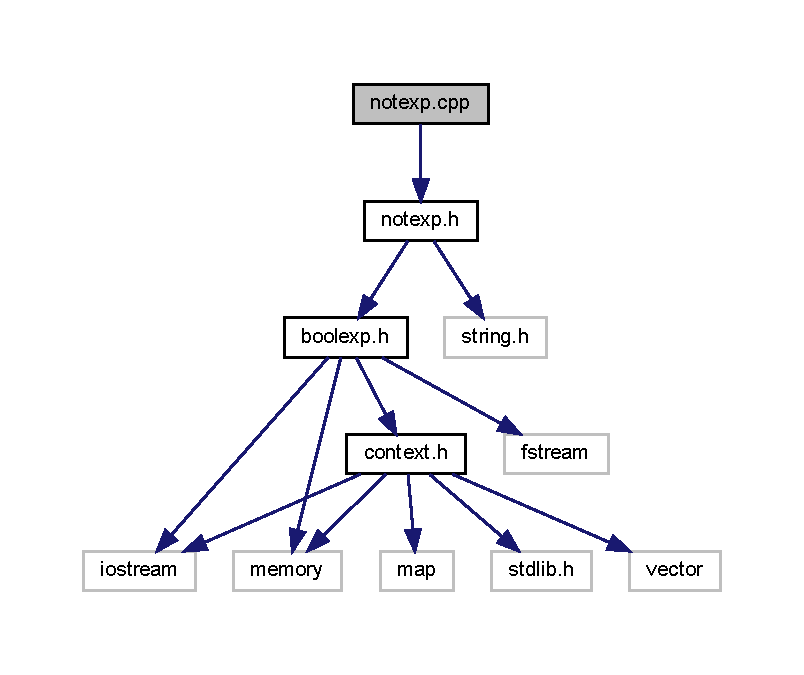
\includegraphics[width=350pt]{notexp_8cpp__incl}
\end{center}
\end{figure}

\hypertarget{notexp_8h}{}\section{notexp.\+h File Reference}
\label{notexp_8h}\index{notexp.\+h@{notexp.\+h}}
{\ttfamily \#include \char`\"{}boolexp.\+h\char`\"{}}\newline
{\ttfamily \#include $<$string.\+h$>$}\newline
Include dependency graph for notexp.\+h\+:
\nopagebreak
\begin{figure}[H]
\begin{center}
\leavevmode
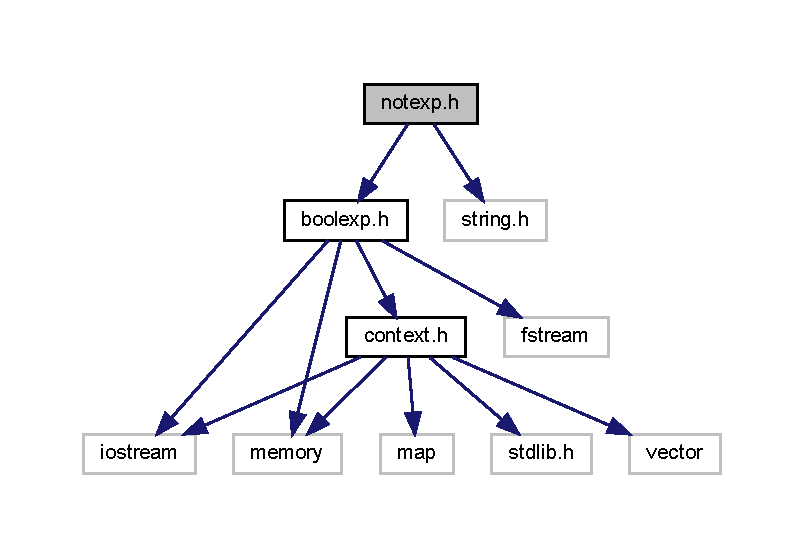
\includegraphics[width=350pt]{notexp_8h__incl}
\end{center}
\end{figure}
This graph shows which files directly or indirectly include this file\+:
\nopagebreak
\begin{figure}[H]
\begin{center}
\leavevmode
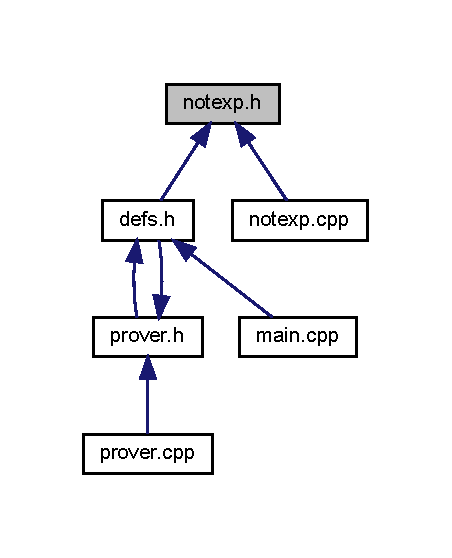
\includegraphics[width=217pt]{notexp_8h__dep__incl}
\end{center}
\end{figure}
\subsection*{Classes}
\begin{DoxyCompactItemize}
\item 
class \mbox{\hyperlink{classNotExp}{Not\+Exp}}
\end{DoxyCompactItemize}

\hypertarget{orexp_8cpp}{}\section{orexp.\+cpp File Reference}
\label{orexp_8cpp}\index{orexp.\+cpp@{orexp.\+cpp}}
{\ttfamily \#include \char`\"{}orexp.\+h\char`\"{}}\newline
Include dependency graph for orexp.\+cpp\+:
\nopagebreak
\begin{figure}[H]
\begin{center}
\leavevmode
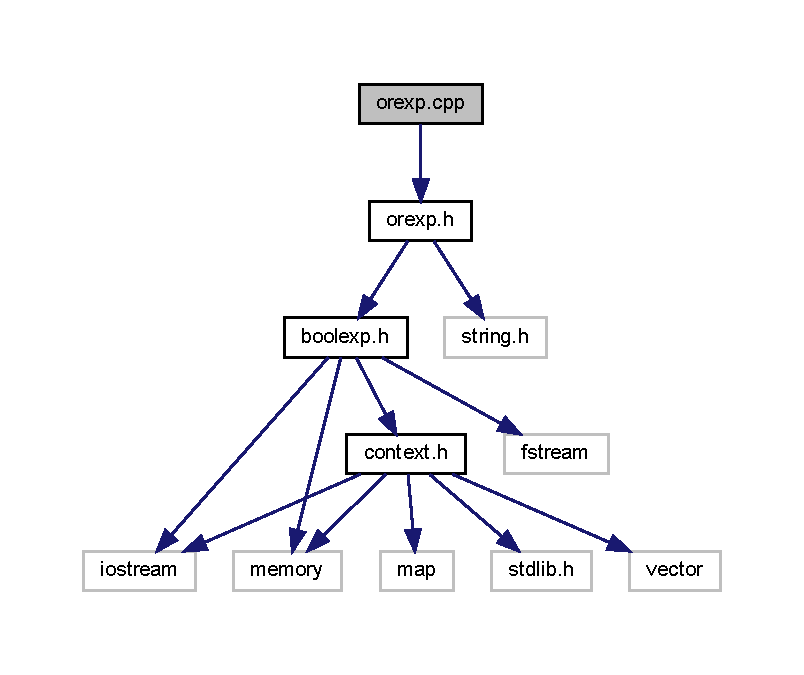
\includegraphics[width=350pt]{orexp_8cpp__incl}
\end{center}
\end{figure}

\hypertarget{orexp_8h}{}\section{orexp.\+h File Reference}
\label{orexp_8h}\index{orexp.\+h@{orexp.\+h}}
{\ttfamily \#include \char`\"{}boolexp.\+h\char`\"{}}\newline
{\ttfamily \#include $<$string.\+h$>$}\newline
Include dependency graph for orexp.\+h\+:
\nopagebreak
\begin{figure}[H]
\begin{center}
\leavevmode
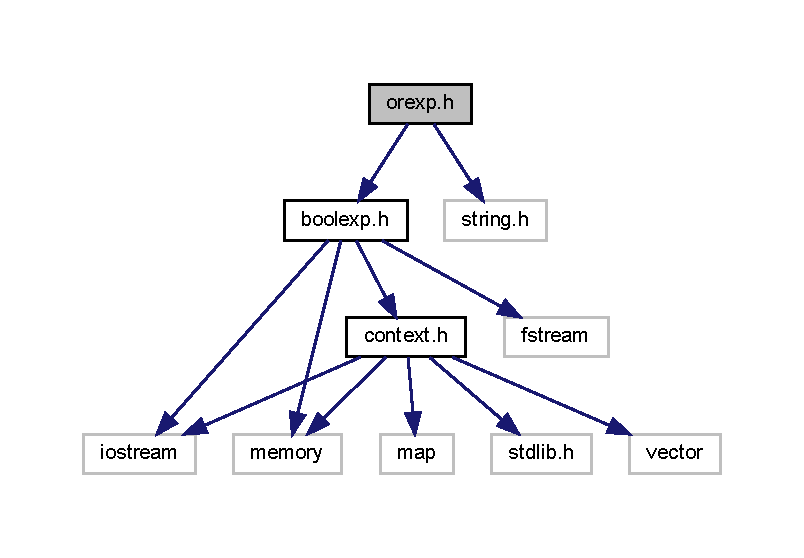
\includegraphics[width=350pt]{orexp_8h__incl}
\end{center}
\end{figure}
This graph shows which files directly or indirectly include this file\+:
\nopagebreak
\begin{figure}[H]
\begin{center}
\leavevmode
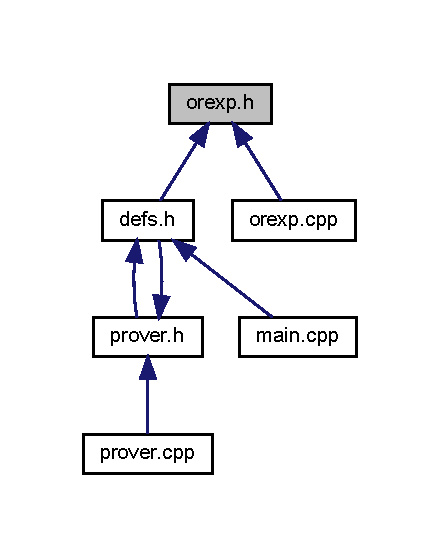
\includegraphics[width=211pt]{orexp_8h__dep__incl}
\end{center}
\end{figure}
\subsection*{Classes}
\begin{DoxyCompactItemize}
\item 
class \mbox{\hyperlink{classOrExp}{Or\+Exp}}
\end{DoxyCompactItemize}

\hypertarget{prover_8cpp}{}\section{prover.\+cpp File Reference}
\label{prover_8cpp}\index{prover.\+cpp@{prover.\+cpp}}
{\ttfamily \#include \char`\"{}prover.\+h\char`\"{}}\newline
Include dependency graph for prover.\+cpp\+:
\nopagebreak
\begin{figure}[H]
\begin{center}
\leavevmode
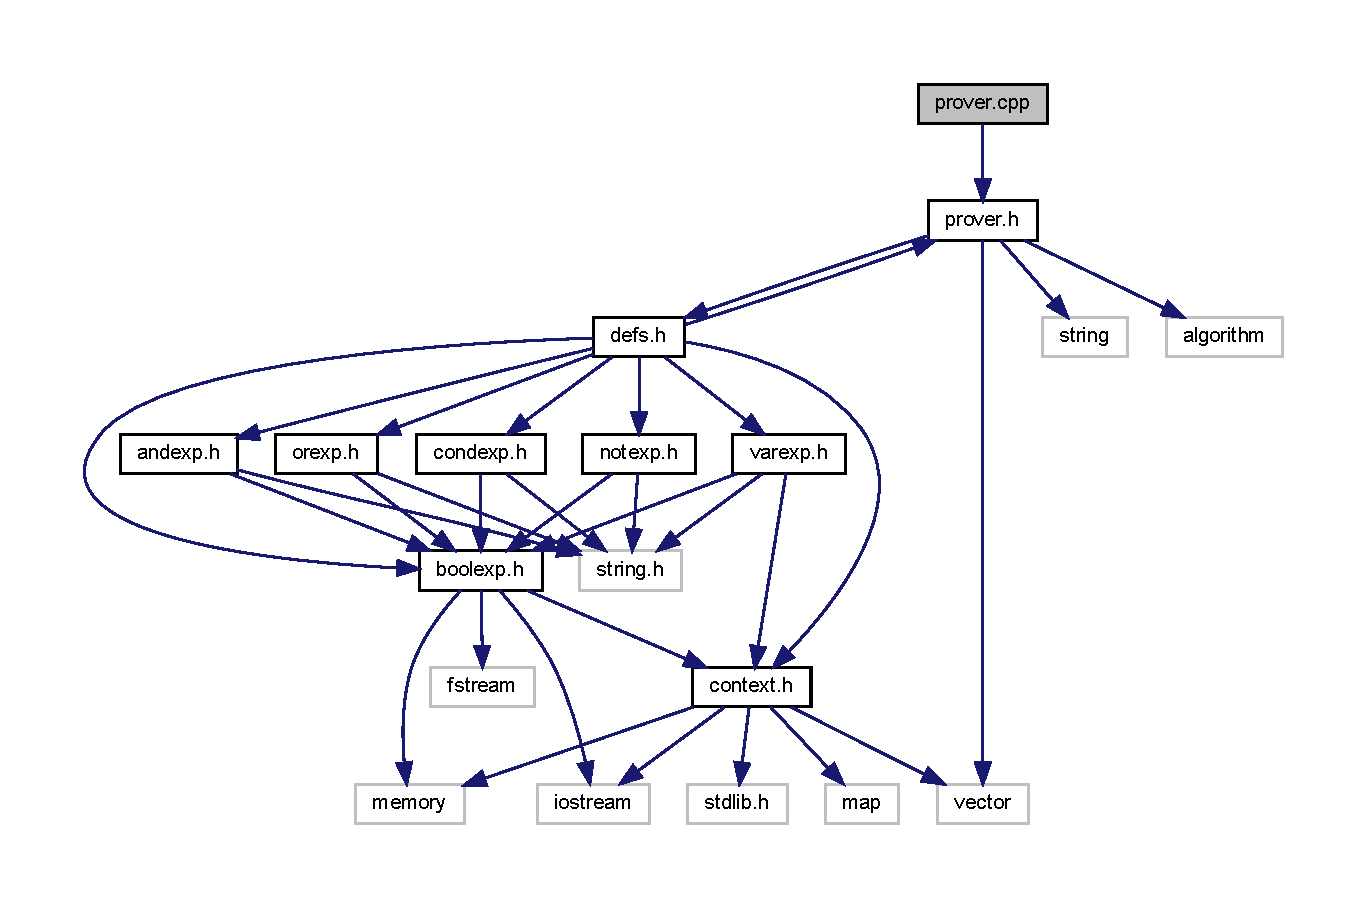
\includegraphics[width=350pt]{prover_8cpp__incl}
\end{center}
\end{figure}

\hypertarget{prover_8h}{}\section{prover.\+h File Reference}
\label{prover_8h}\index{prover.\+h@{prover.\+h}}
{\ttfamily \#include \char`\"{}defs.\+h\char`\"{}}\newline
{\ttfamily \#include $<$vector$>$}\newline
{\ttfamily \#include $<$string$>$}\newline
{\ttfamily \#include $<$algorithm$>$}\newline
Include dependency graph for prover.\+h\+:
\nopagebreak
\begin{figure}[H]
\begin{center}
\leavevmode
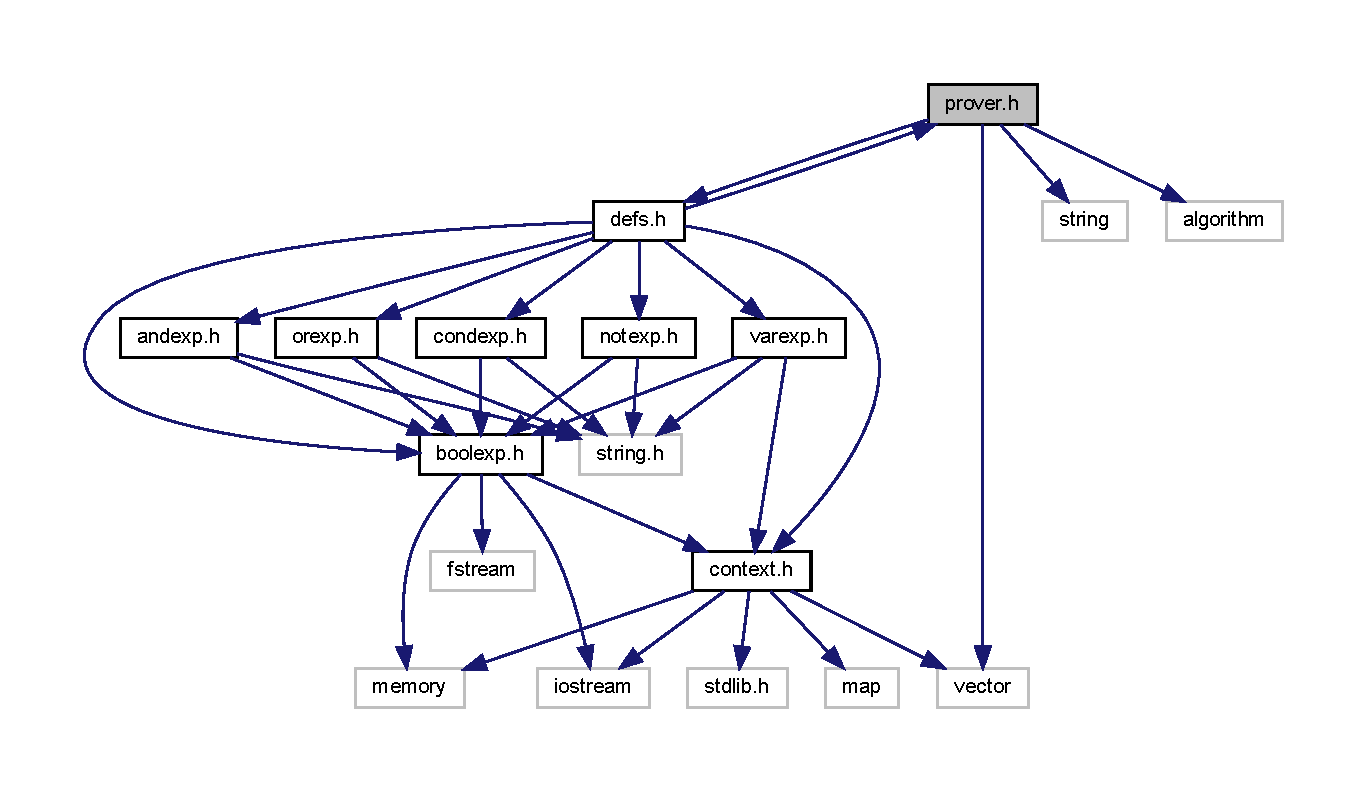
\includegraphics[width=350pt]{prover_8h__incl}
\end{center}
\end{figure}
This graph shows which files directly or indirectly include this file\+:
\nopagebreak
\begin{figure}[H]
\begin{center}
\leavevmode
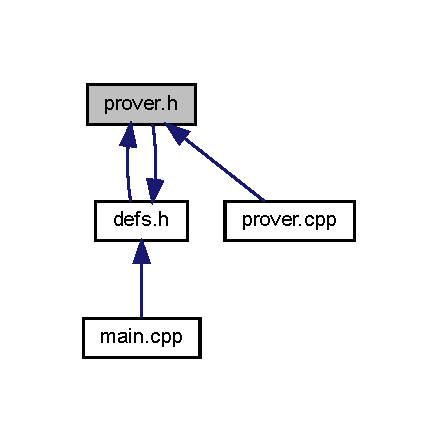
\includegraphics[width=210pt]{prover_8h__dep__incl}
\end{center}
\end{figure}
\subsection*{Classes}
\begin{DoxyCompactItemize}
\item 
class \mbox{\hyperlink{classProver}{Prover}}
\end{DoxyCompactItemize}

\hypertarget{varexp_8cpp}{}\section{varexp.\+cpp File Reference}
\label{varexp_8cpp}\index{varexp.\+cpp@{varexp.\+cpp}}
{\ttfamily \#include \char`\"{}varexp.\+h\char`\"{}}\newline
Include dependency graph for varexp.\+cpp\+:
\nopagebreak
\begin{figure}[H]
\begin{center}
\leavevmode
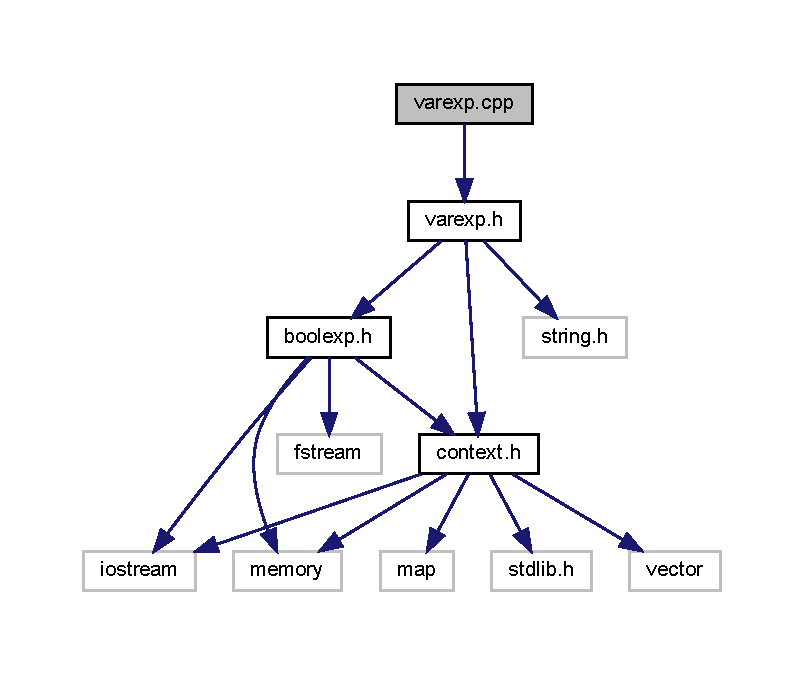
\includegraphics[width=350pt]{varexp_8cpp__incl}
\end{center}
\end{figure}

\hypertarget{varexp_8h}{}\section{varexp.\+h File Reference}
\label{varexp_8h}\index{varexp.\+h@{varexp.\+h}}
{\ttfamily \#include \char`\"{}boolexp.\+h\char`\"{}}\newline
{\ttfamily \#include \char`\"{}context.\+h\char`\"{}}\newline
{\ttfamily \#include $<$string.\+h$>$}\newline
Include dependency graph for varexp.\+h\+:
\nopagebreak
\begin{figure}[H]
\begin{center}
\leavevmode
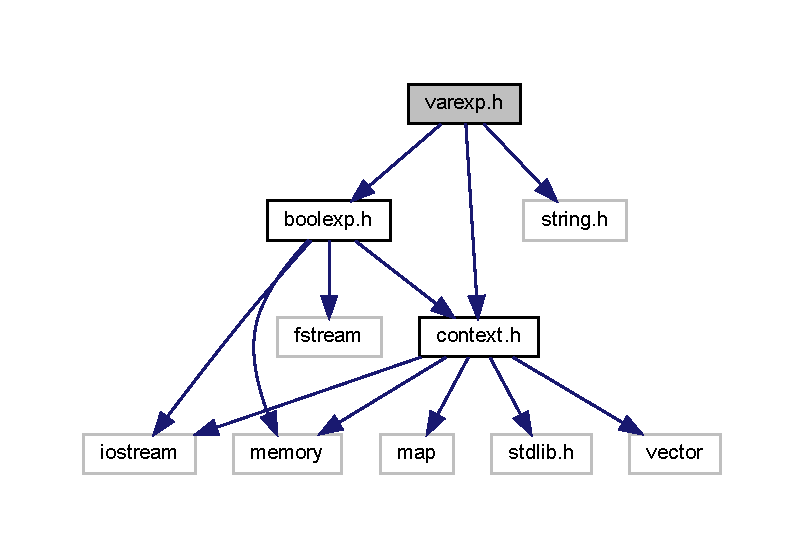
\includegraphics[width=350pt]{varexp_8h__incl}
\end{center}
\end{figure}
This graph shows which files directly or indirectly include this file\+:
\nopagebreak
\begin{figure}[H]
\begin{center}
\leavevmode
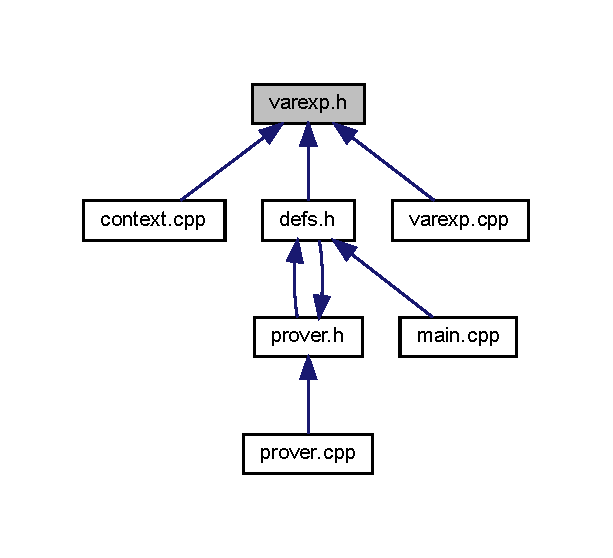
\includegraphics[width=294pt]{varexp_8h__dep__incl}
\end{center}
\end{figure}
\subsection*{Classes}
\begin{DoxyCompactItemize}
\item 
class \mbox{\hyperlink{classVarExp}{Var\+Exp}}
\end{DoxyCompactItemize}

%--- End generated contents ---

% Index
\backmatter
\newpage
\phantomsection
\clearemptydoublepage
\addcontentsline{toc}{chapter}{Index}
\printindex

\end{document}
